% Options for packages loaded elsewhere
\PassOptionsToPackage{unicode}{hyperref}
\PassOptionsToPackage{hyphens}{url}
%
\documentclass[
]{book}
\usepackage{amsmath,amssymb}
\usepackage{lmodern}
\usepackage{iftex}
\ifPDFTeX
  \usepackage[T1]{fontenc}
  \usepackage[utf8]{inputenc}
  \usepackage{textcomp} % provide euro and other symbols
\else % if luatex or xetex
  \usepackage{unicode-math}
  \defaultfontfeatures{Scale=MatchLowercase}
  \defaultfontfeatures[\rmfamily]{Ligatures=TeX,Scale=1}
\fi
% Use upquote if available, for straight quotes in verbatim environments
\IfFileExists{upquote.sty}{\usepackage{upquote}}{}
\IfFileExists{microtype.sty}{% use microtype if available
  \usepackage[]{microtype}
  \UseMicrotypeSet[protrusion]{basicmath} % disable protrusion for tt fonts
}{}
\makeatletter
\@ifundefined{KOMAClassName}{% if non-KOMA class
  \IfFileExists{parskip.sty}{%
    \usepackage{parskip}
  }{% else
    \setlength{\parindent}{0pt}
    \setlength{\parskip}{6pt plus 2pt minus 1pt}}
}{% if KOMA class
  \KOMAoptions{parskip=half}}
\makeatother
\usepackage{xcolor}
\usepackage{longtable,booktabs,array}
\usepackage{calc} % for calculating minipage widths
% Correct order of tables after \paragraph or \subparagraph
\usepackage{etoolbox}
\makeatletter
\patchcmd\longtable{\par}{\if@noskipsec\mbox{}\fi\par}{}{}
\makeatother
% Allow footnotes in longtable head/foot
\IfFileExists{footnotehyper.sty}{\usepackage{footnotehyper}}{\usepackage{footnote}}
\makesavenoteenv{longtable}
\usepackage{graphicx}
\makeatletter
\def\maxwidth{\ifdim\Gin@nat@width>\linewidth\linewidth\else\Gin@nat@width\fi}
\def\maxheight{\ifdim\Gin@nat@height>\textheight\textheight\else\Gin@nat@height\fi}
\makeatother
% Scale images if necessary, so that they will not overflow the page
% margins by default, and it is still possible to overwrite the defaults
% using explicit options in \includegraphics[width, height, ...]{}
\setkeys{Gin}{width=\maxwidth,height=\maxheight,keepaspectratio}
% Set default figure placement to htbp
\makeatletter
\def\fps@figure{htbp}
\makeatother
\setlength{\emergencystretch}{3em} % prevent overfull lines
\providecommand{\tightlist}{%
  \setlength{\itemsep}{0pt}\setlength{\parskip}{0pt}}
\setcounter{secnumdepth}{5}
\usepackage{booktabs}
\ifLuaTeX
  \usepackage{selnolig}  % disable illegal ligatures
\fi
\usepackage[]{natbib}
\bibliographystyle{plainnat}
\IfFileExists{bookmark.sty}{\usepackage{bookmark}}{\usepackage{hyperref}}
\IfFileExists{xurl.sty}{\usepackage{xurl}}{} % add URL line breaks if available
\urlstyle{same} % disable monospaced font for URLs
\hypersetup{
  pdftitle={Monitorização dos PIICIE: uma proposta de avaliação para além da parametrização do sucesso},
  pdfauthor={RELATÓRIO FINAL},
  hidelinks,
  pdfcreator={LaTeX via pandoc}}

\title{Monitorização dos PIICIE: uma proposta de avaliação para além da parametrização do sucesso}
\usepackage{etoolbox}
\makeatletter
\providecommand{\subtitle}[1]{% add subtitle to \maketitle
  \apptocmd{\@title}{\par {\large #1 \par}}{}{}
}
\makeatother
\subtitle{Financiado pelo Programa Operacional de Assistência Técnica (POAT) 2020, código do projeto POAT-01-6177-FEDER-000053}
\author{RELATÓRIO FINAL}
\date{12 de dezembro de 2022}

\begin{document}
\maketitle

{
\setcounter{tocdepth}{1}
\tableofcontents
}
\hypertarget{resumo-abstract}{%
\chapter*{\texorpdfstring{\textbf{Resumo (Abstract)}}{Resumo (Abstract)}}\label{resumo-abstract}}
\addcontentsline{toc}{chapter}{\textbf{Resumo (Abstract)}}

\textbf{Resumo}

A breve existência dos Planos Integrados e Inovadores de Combate ao Insucesso Escolar (PIICIE), em parte coincidente com uma conturbada conjuntura, não deve comprometer os esforços de avaliação do seu processo e dos seus resultados. Pelo contrário, este afigura-se como o momento ideal para uma aferição tão rigorosa quanto possível da sua implementação, bem como dos seus desafios e lacunas.

Antes de mais, surge uma necessidade premente de contextualizar nacional, regional e localmente a problemática do insucesso escolar, principalmente através dos indicadores de resultado dos PIICIE (taxa de retenção e desistência e taxa de alunos com níveis negativos), enriquecidos pelo recente indicador de equidade.

Adotando uma lente micro, segue-se uma análise mais focada no caso de estudo demonstrador da metodologia: Santa Maria da Feira. Não só se caracterizam as ações compreendidas no respetivo PIICIE, recorrendo à informação disponível, como se olha para o desempenho do município nos indicadores de resultado e de realização contratualizados. Todo o processo de recolha de informação evidenciou as fragilidades e os desafios de uma rigorosa avaliação. Com uma ambiciosa proposta de indicadores colide a realidade da insuficiente estrutura de dados, pelo que o projeto acaba, em alguns pontos, por ser mais propositivo do que demonstrador.

Ainda assim, toda a informação que pôde ser recolhida e trabalhada surge, por fim, apresentada em painéis de informação que, idealmente, deveria constar nos canais de comunicação das entidades beneficiárias. Do projeto resulta, ainda, um conjunto final de \emph{policy recommendations} (recomendação de políticas) que deverão ser consideradas nos planos de promoção do sucesso a implementar durante o quadro 2021-2027.

\begin{center}\rule{0.5\linewidth}{0.5pt}\end{center}

\textbf{Abstract}

The so far short life of the \emph{Planos Integrados e Inovadores de Combate ao Insucesso Escolar} (PIICIE), overlapping with a critical juncture, must not curb the evaluation of their implementation process and results. On the contrary, this is the ideal moment for an evaluation as thorough as possible of their implementation, their challenges and gaps.

Firstly, there is a pressing need to contextualize school failure problematics nationally, regionally, and locally, especially regarding the PIICIE's outcome indicators (failure and dropout rates, and low achievement rates), enhanced by the recent indicator of educational equity.

While embracing a micro lens, the following step is focused on the case study that intends to illustrate the methodology: the municipality of Santa Maria da Feira. The actions covered by the PIICIE are described and characterized by resorting to the available information. Besides, we take a look at the municipality's performance regarding outcome and output indicators. The data collection process highlighted the weaknesses and challenges of a thorough evaluation. The reality of insufficient data collides with an ambitious proposal of indicators, so the project ends up, in some points, being more propositional than demonstrative.

Nonetheless, the data that could be collected is presented in dashboards that should be further used by the beneficiaries. The project also results in a range of policy recommendations to be considered within the plans for school success to be implemented during the 2021-2027 framework.

\begin{center}\rule{0.5\linewidth}{0.5pt}\end{center}

\hypertarget{introduuxe7uxe3o}{%
\chapter{\texorpdfstring{\textbf{Introdução}}{Introdução}}\label{introduuxe7uxe3o}}

\hypertarget{problematizauxe7uxe3o}{%
\section{\texorpdfstring{\textbf{Problematização}}{Problematização}}\label{problematizauxe7uxe3o}}

O combate ao abandono escolar precoce, e ao insucesso escolar mais genericamente compreendido, foi assumido como uma das principais prioridades educativas a considerar pela União Europeia durante o quadro financeiro plurianual 2014 -- 2020 (Nóvoa, 2013). Portugal, aliás, apresentava preocupantes taxas de abandono escolar precoce, tendo posteriormente trilhado uma evolução notável. O Programa Nacional de Promoção do Sucesso Escolar (PNPSE), criado em 2016, propõe várias ações de combate ao insucesso, quer cofinanciadas (como os PIICIE e os TEIP), quer não cofinanciadas (tais como os Planos de Ação Estratégica dos Agrupamentos). Tal como estabelece desde logo a Resolução do Conselho de Ministros n.º 23/2016, que oficializa o PNPSE, o programa assenta

\begin{quote}
``no princípio de que são as comunidades educativas quem melhor conhece os seus contextos, as dificuldades e potencialidades, sendo, por isso, quem está melhor preparado para encontrar soluções locais e conceber planos de ação estratégica, pensados ao nível de cada escola, com o objetivo de melhorar as práticas educativas e as aprendizagens dos alunos''
\end{quote}

Estes princípios têm já vindo a orientar a formulação de instrumentos de política educativa local, designadamente Cartas Educativas e Planos Estratégicos Educativos Municipais (Decreto-Lei n.o 7/2003, de 15 de janeiro; Decreto-Lei n.o 72/2015, de 11 de maio; Decreto-Lei n.o 21/2019, de 30 de janeiro), cuja componente de monitorização tem também vindo a ser promovida. O exercício a que este trabalho se propõe surge, justamente, na sequência do envolvimento de parte da equipa em tais projetos, junto de municípios portugueses, assim tendo já conhecimento prévio de alguns desafios.

Não obstante, a proposta deste projeto, feita em sede de candidatura, contemplava um empreendimento mais ambicioso do que aquele que foi possível concretizar, muito por via das limitações associadas aos dados disponíveis. Assim, conquanto o relatório cumpre o propósito de apresentação de uma ``proposta de avaliação para além da parametrização do sucesso'', não demonstra a monitorização, uma vez que o caso de estudo selecionado (o PIICIE de Santa Maria da Feira) teve o seu término a 31 de dezembro de 2021, pouco depois do início do presente projeto. Focando a avaliação, este caso de estudo foi fulcral para identificar os desafios e as oportunidades que surgem ao longo do processo de avaliação de um programa cofinanciado de promoção do sucesso escolar. Considera-se, no entanto, que a ``avaliação para além da parametrização do sucesso'' foi cumprida na medida do possível, uma vez que foram encetados vários esforços de detalhada caracterização, quer do território, quer das ações enquadradas pelo PIICIE municipal.

O trabalho foi enriquecido com metodologias de análise e tratamento estatístico que, ainda que não contempladas na memória descritiva da candidatura, constituem propostas de investigação quer sobre o insucesso escolar, quer sobre os cofinanciamentos na promoção do sucesso.

Por fim, procurando propor medidas e caminhos atenuadores de duas grandes fragilidades identificadas nestes processos, os principais \emph{outputs} do projeto são:

\begin{itemize}
\tightlist
\item
  A construção de painéis de informação que permitam apresentar, de forma tão intuitiva e interativa quanto possível, o desempenho educativo no território considerado e a caracterização das ações implementadas, assim procurando melhorar a transparência e divulgação dos PIICIE, numa lógica integrada face à realidade educativa;\\
\item
  A elaboração de \emph{policy recommendations}, decorrentes de todo o processo subjacente a este projeto, e que permitam construir alguma aprendizagem que seja mobilizada para os futuros programas de promoção do sucesso escolar.
\end{itemize}

Ainda que, neste âmbito, a proposta para o Programa Demografia, Qualificações e Inclusão apenas mencione o Plano 21\textbar23 Escola+ (Portugal 2030, 2022, p.~56), será recomendável a formulação de outras medidas no período de vigência do atual quadro comunitário, tais como os Planos Intermunicipais de Promoção do Sucesso Escolar (CCDR-Centro, 2022; CCDR-Norte, 2022).

Deve partir-se para a leitura do restante relatório com a consciência de que, não obstante a pretensão demonstradora, o projeto tem como maior força o seu caráter propositivo. Aliás, o reforço da componente propositiva surge como compensação face à impossibilidade (muito por via da indisponibilidade de dados e do impacto pandémico) de demonstração rigorosa da metodologia. Deste modo, considera-se que do projeto resultam, fundamentalmente, 4 principais áreas de proposta:

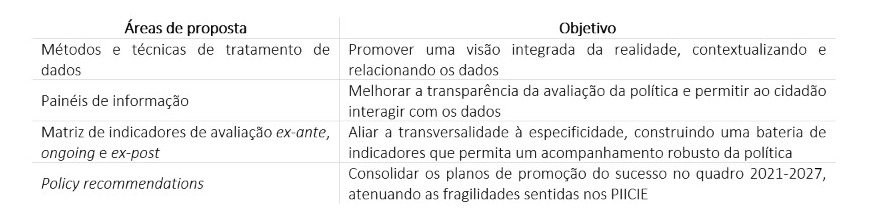
\includegraphics{C:/Users/julio/Documents/bookPoat/imagensRelatorio/f2017e0e-c5d0-4088-b8a1-78d738a5e183.jpg}

\begin{figure}
\centering
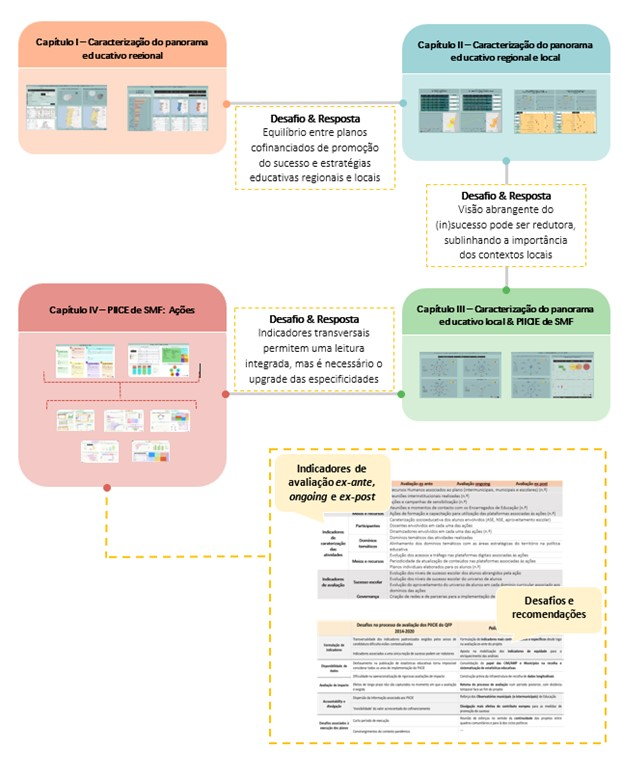
\includegraphics{C:/Users/julio/Documents/bookPoat/imagensRelatorio/Imagem1.jpg}
\caption{FIGURA 1: Diálogo proposto entre Painéis de Informação, Indicadores de Avaliação e Recomendações na implementação de estratégias de monitorização do (in)sucesso escolar - FONTE: GETIN-UA}
\end{figure}

\hypertarget{metodologia}{%
\section{\texorpdfstring{\textbf{Metodologia}}{Metodologia}}\label{metodologia}}

Este projeto adota, ainda assim, uma metodologia que parte de indicadores mais genéricos (associados aos indicadores de resultado e realização dos Programas Operacionais) e propõe indicadores específicos para as ações. Procura privilegiar-se a territorialização e contextualização dos indicadores, ainda que partindo daqueles mais padronizados. A informação será apresentada através de painéis (dashboards) que surgem como exemplificativos de uma estratégia de tratamento e apresentação de dados que permita situar o território (face a outras unidades territoriais) e caracterizá-lo, do ponto de vista da implementação deste projeto específico (o PIICIE). \textbf{Idealmente, a construção dos \emph{dashboards} seria feita por meio da interoperabilidade de sistemas, assumindo que a informação a preencher pelas escolas (quer para a tutela, quer para a autoridade de gestão dos fundos comunitários) pode ser mobilizada, ao invés de multiplicada.}

\hypertarget{construuxe7uxe3o-dos-dashboards}{%
\subsection{\texorpdfstring{\textbf{Construção dos \emph{dashboards} }}{Construção dos dashboards }}\label{construuxe7uxe3o-dos-dashboards}}

Para Wickham e Grolemund (2019, p.~473), \emph{dashboards} são uma maneira favorável de comunicar grandes quantidades de informação visualmente e rapidamente. Gartner (2020, p.~1) destaca que os dashboards agregam indicadores de desempenho (\emph{Key Performance Indicators - KPIs}), tornando possível serem utilizados rapidamente por todos os utilizadores antes de uma eventual exploração adicional através de ferramentas de análise. Os \emph{dashboards} apresentam a informação combinando texto e opções gráficas num painel. Na maioria das vezes, são as opções gráficas que acabam por se destacar, pois comunicam a informação de forma mais intuitiva e inteligível.

Na etapa de tratamento e análise de dados, que precede a construção dos \emph{dashboards}, utilizou-se o \emph{software} estatístico R. Este \emph{software} é uma linguagem e ambiente para computação estatística e representação visual da informação tratada, permitindo aplicar uma ampla variedade de métodos (e.g.~modelação linear e não linear, testes estatísticos clássicos, análise de séries temporais, classificação, agrupamento). Para a construção dos dashboards utilizou-se a ferramenta \emph{Microsoft Power BI}. Segundo a informação disponível no sítio da \emph{Microsoft}, o \emph{Power BI} é uma coleção de serviços de \emph{software}, aplicações e conectores que funcionam em conjunto para transformar as origens de dados não relacionadas em informações coerentes, visualmente envolventes e interativas. O \emph{Power BI} permite ligar-se facilmente às origens de dados, visualizar e descobrir o que é importante, bem como partilhar os seus conteúdos com qualquer pessoa.

\begin{figure}
\centering
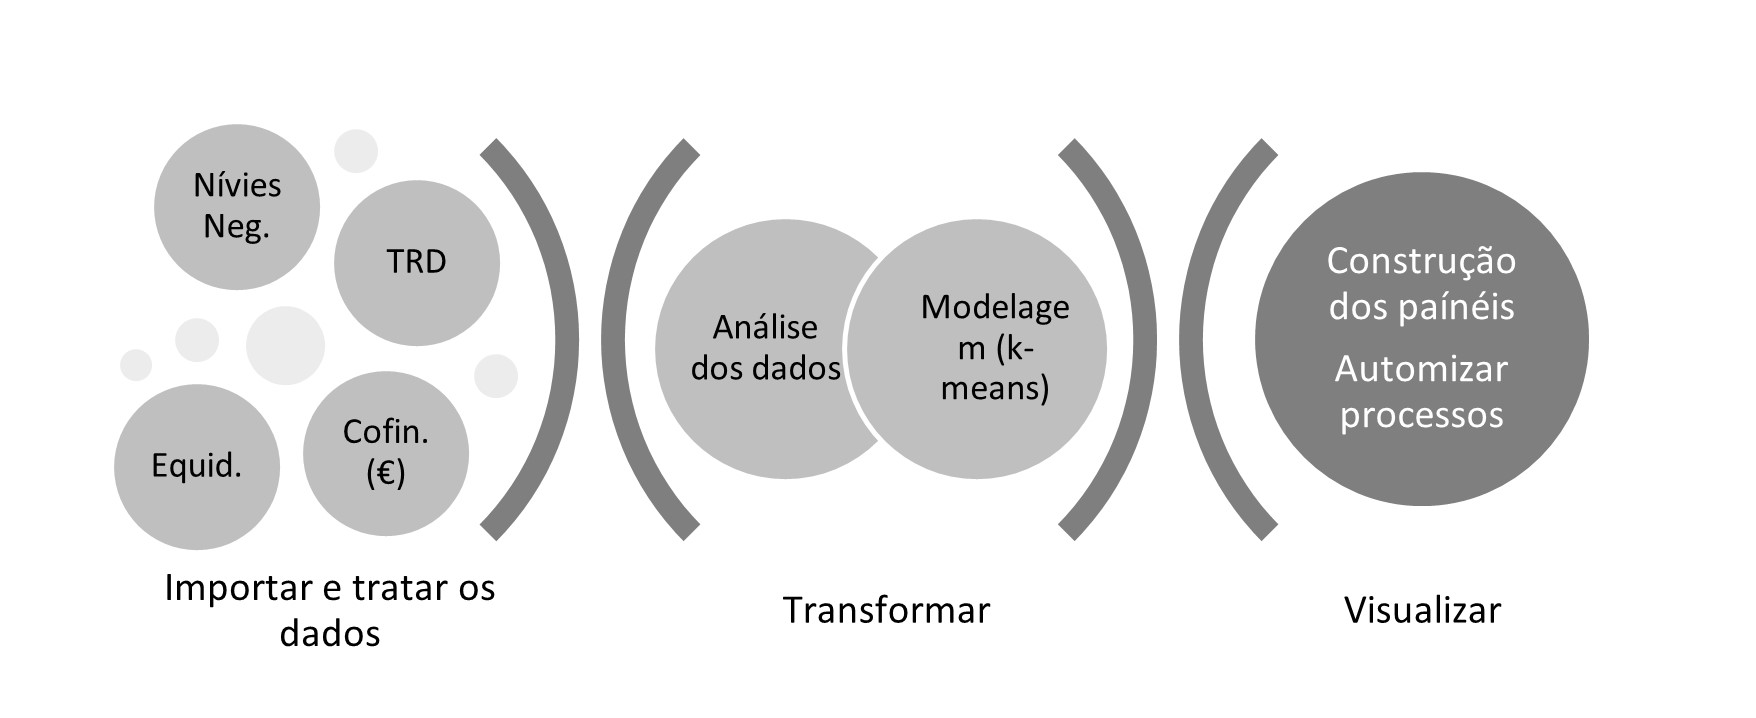
\includegraphics{C:/Users/julio/Documents/bookPoat/imagensRelatorio/Imagem2.jpg}
\caption{FIGURA 2: O ciclo da Ciência dos Dados - FONTE: Adaptado de Wickham e Grolemund (2019)}
\end{figure}

A figura anterior apresenta as etapas dos processos de recolha, tratamento e análise de dados nacionais sobre o (in)sucesso escolar, numa perspetiva de utilização das ferramentas computacionais de maneira intercooperativa e multiplataforma. Grande parte dos dados disponibilizados para a análise estavam distribuídos em diversas plataformas eletrónicas, diferentes suportes de armazenamento de dados e estruturas de dados também elas distintas (fazer referência às mais importantes). Este formato não se mostrou ser o ideal para os objetivos do projeto, colocando desafios em diferentes etapas da sua concretização. Foi necessário um esforço adicional no tratamento de dados, de modo a transformá-los numa estrutura triangular, tanto para a construção de \emph{dashboards}, quanto para a modelação matemática proposta.

\hypertarget{diagnuxf3stico-do-insucesso-escolar}{%
\subsection{\texorpdfstring{\textbf{Diagnóstico do (in)sucesso escolar}}{Diagnóstico do (in)sucesso escolar}}\label{diagnuxf3stico-do-insucesso-escolar}}

\textbf{\emph{Tendências e padrões no sucesso}}

O diagnóstico de tendências e padrões ao nível do sucesso escolar foi desenvolvido tendo como objetivo último caracterizar o território de estudo -- o município de Santa Maria da Feira (SMF). As análises produzidas nos diferentes capítulos dos \emph{dashboards} refletem-se nos painéis de informação elaborados (2 painéis por capítulo). A caracterização do panorama educativo parte assim de uma visão geral do território nacional, para as regiões de referência de SMF, a Região Norte (NUTSII) e a Área Metropolitana do Porto (NUTS III), afunilando no contexto específico do município. \textbf{Recomenda-se que a leitura desta secção seja acompanhada dos painéis.}

\textbf{1. Capítulo I - Caracterização do panorama educativo nacional}

O capítulo I desenvolve-se em torno do mapeamento do indicador de cofinanciamento (1º painel) e de uma análise de similaridades, que combina indicadores gerais de resultado com outros indicadores de caracterização socioeducativa relevantes na definição de clusters territoriais (2º painel).

O indicador de cofinanciamento foi incorporado no modelo seguindo critérios de distribuição dos recursos em M/€ correspondentes às operações PIICIE aprovadas, intermunicipais e municipais. Neste exercício foram considerados os valores alocados diretamente aos municípios, juntamente com o resultado do rácio dos recursos intermunicipais (NUTSIII). A incorporação no modelo segue a proporcionalidade de alunos em cada nível de ensino, incluindo a educação pré-escolar.

Já a análise de similaridades, ou de agrupamento, permitiu formar \emph{clusters} territoriais, que decorrem do reconhecimento de semelhanças entre municípios de Portugal Continental, recorrendo até 4 indicadores de 2017/18 a 2019/20: i) total de alunos, ii) média das taxas de retenção e desistência (TRD), iii) equidade\footnote{\textbf{Indicador de Equidade} -- O indicador de equidade pode assumir valores negativos, motivo pelo qual o eixo dos YY inclui valores \textless{} 0. ``Diferença entre a \% de conclusão no tempo esperado na região e a média nacional comparável, em pontos percentuais.'' A média nacional ``é calculada com os alunos do país que, ao entrarem no 3.º ciclo, tinham um perfil semelhante ao dos alunos da região, em termos de apoios ASE, idade à entrada no ciclo, habilitação da mãe e categoria da escola frequentada relativamente à percentagem de alunos com apoio ASE. O objetivo é enquadrar os resultados dos alunos com apoio ASE na região com uma média nacional apropriada.'' Fonte: PORTAL INFOESCOLAS / Produção dos indicadores: DGEEC/Medu. \url{https://infoescolas.medu.pt/bds.asp}} e iv) rácio entre cofinanciamento de operações PIICIE e total de alunos do ensino básico, ensino secundário em cursos científico-humanísticos (CCH) e em cursos profissionais\footnote{\textbf{Indicador do Rácio entre financiamento PIICIE e Alunos Inscritos por níveis de ensino} -- Nos valores de cofinanciamento, é considerado o fundo total aprovado em €, de 2016 a 2020. Este indicador foi calculado pela equipa. \textbf{Fonte:} Financiamento PIICIE -- Projetos Aprovados nos PO Reginais, de acordo com a base de dados atualizada a 31/08/2021 / Alunos Inscritos por níveis de ensino -- DGEEC.} (Prof.). Duas análises de similaridade foram realizadas, com representações gráficas que permitem confrontar as diferenças ao nível da formação dos \emph{clusters}: a \textbf{similaridade 1}que considera o total de alunos (eixo dos YY), a TRD (eixo dos XX) e a equidade (diâmetro dos círculos); e a \textbf{similaridade 2}, que inclui indicadores de cofinanciamento (eixo dos YY), TRD (eixo dos XX) e equidade (diâmetro dos círculos).

A análise de similaridades pode ser entendida como um processo que permite descobrir relações existentes entre os exemplares de um conjunto de dados descritos por uma série de características (atributos descritivos). As análises realizadas pelos algoritmos que implementam estratégias para agrupamento procuram por similaridades ou diferenças entre exemplares, qualificadas através de medidas de distância (quanto menor for a distância entre dois exemplares, maior será a similaridade). Assim, exemplares similares serão associados a um mesmo grupo e exemplares dissimilares a grupos diferentes. No final de um algoritmo de agrupamento, uma estrutura será formada de maneira a que a similaridade intragrupos tenha sido maximizada e a similaridade intergrupos minimizada. Este estudo utiliza o \emph{k-means}, que agrupa os dados em grupos de variância igual em relação aos pontos médios, chamados centróides (Silva, Peres e Boscarioli, 2021 \& Sampaio, 2018).

\textbf{2. Capítulo II -- Caracterização do panorama educativo regional e local}

Ao nível do capítulo II, duas análises estiveram na base da elaboração dos painéis de informação partindo dos indicadores gerais de resultado indicados nos avisos de candidatura do PIICIE: i) uma análise regional dos municípios da Área Metropolitana do Porto (AMP), ao nível das Taxas de Níveis Negativos (TNN) a pelo menos uma disciplina e das Taxas de Retenção e Desistência (TRD) (1º painel); e ii) uma análise à escala local dos 9 Agrupamentos de Escolas (AE) do município de SMF (2º painel).

Para esta análise, foram utilizadas bases de dados estatísticos de diferentes instituições oficiais, que cobrem períodos distintos e com diferentes níveis de desagregação. Os dados relativos aos alunos com níveis negativos apenas estavam disponíveis para os 17 municípios da AMP (NUTSIII), de 2014/2015 a 2019/2020, desagregados por escola e para o 2º e 3º CEB. Já a informação relativa aos alunos retidos e desistentes, abrangiam todos os municípios da Região Norte (NUTSII), num total de 86 municípios, de 2014/2015 a 2018/2019, desagregada também por escola para todos os níveis do Ensino Básico e Secundário. No 1º painel, optou-se por modelar os dados e apresentar os indicadores apenas para os territórios da AMP, permitindo a respetiva análise e espacialização à escala da NUTSIII e seus municípios, numa perspetiva comparada. A espacialização dos dois indicadores gerais de desempenho é condicional às respetivas unidades temporais. Além dos dados da AMP, no 2º painel, é possível a análise e espacialização das TNN e TRD por AE do município de estudo e suas escolas.

\textbf{3. Capítulo III -- Caracterização do panorama educativo local \& PIICIE de SMF}

O capítulo III é desenvolvido com base numa análise integrada ao nível do PIICIE de SMF. Esta análise articula, no 1º painel, os indicadores gerais de desempenho (TNN e TRD) e indicadores gerais de caracterização do território de estudo (Equidade e \% de alunos com ASE que concluíram os estudos no tempo esperado). Deste modo, acredita-se ser possível caracterizar os 9 Agrupamentos de Escolas (AE) do município de SMF à luz de informação contextual relevante, quer ao nível da dimensão do desempenho escolar, quer de uma dimensão mais lata ligada à componente socioeducativa. Os dados apenas são apresentados para os anos letivos comuns aos indicadores utlizados -- 2017/18 e 2018/19.

No 2º painel, estão presentes os 2 indicadores gerais de desempenho (TNN e TRD) e 4 indicadores específicos do PIICIE de SMF estimados pela equipa: i) \% de participantes em cada uma das 6 ações face ao total de participantes em cada AE; ii) \% de participantes em cada uma das 6 ações face ao total de alunos em cada AE; iii) \% de participantes nas 6 ações face ao total de participantes em cada AE; e iv) \% de participantes nas 6 ações face ao total de alunos de cada AE. A utilização conjunta destes indicadores, permite fazer um diagnóstico mais articulado, combinando indicadores da realização efetiva das ações do PIICIE e indicadores de desempenho dos contextos específicos dos AE. Nos gráficos 1 e 2, são apresentadas TNN e TRD médias, considerando todos os ciclos (do 1ºCEB ao Secundário em ambas as taxas) e todos os anos letivos disponíveis (2014/15-2019/20 e 2014/15-2018/19, respetivamente), e indicadores sobre os participantes no PIICIE, abrangendo todas as ações e todo o período de implementação. Nos gráficos 3 e 4, as TNN e as TRD reportam a um ano letivo específico, 2018/19, onde a primeira é representada pelo diâmetro do círculo e a segunda no eixo dos XX; já os participantes surgem no eixo dos YY e são passíveis de análise por ano letivo do PIICIE.

Numa lógica sequencial face ao capítulo III e anteriores, surge o capítulo IV, que se centra na componente descritiva de cada uma das ações do PIICIE de SMF. O capítulo IV é constituído por 7 painéis: 2 mais gerais que sintetizam informações de todas as ações (e.g.~total de participantes por ano letivo ou parceiros envolvidos em cada ação) e outros 5 painéis específicos (um por ação, com exceção do observatório). Nos painéis exclusivos de cada ação procurou reunir-se toda a informação coligida sobre as ações, através de indicadores tipificados (participantes, parceiros, atividades e domínios temáticos), mas também específicas de cada ação (e.g.~acessos à plataforma EDUFEIRA@. na ação 4 -- Educação 5.0). Pretende-se assim que seja possível averiguar a \emph{performance} e os resultados das ações, tendo em conta os seus objetivos e público-alvo.

\begin{figure}
\centering
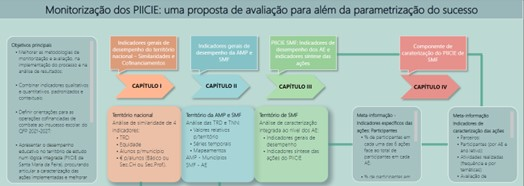
\includegraphics{C:/Users/julio/Documents/bookPoat/imagensRelatorio/figura27.jpg}
\caption{FIGURA 3: Roteiro geral dos Painéis de Caracterização do Panorama Educativo - FONTE: GETIN-UA}
\end{figure}

\textbf{Fatores de influência do sucesso}

A análise de autocorrelação espacial foi aplicada aos municípios da Região Norte -- NUTSII de referência do município de estudo -- e contribuiu para a identificação de possíveis fatores de influência do sucesso escolar nesses territórios. De forma sucinta, a análise desenvolvida consiste em perceber a influência de municípios vizinhos no comportamento de uma determinada variável dependente num município específico e apurar quais os fatores que melhor permitem explicar o comportamento dessa variável -- neste caso, foram analisadas as taxas de retenção e desistência (TRD). Através da linguagem de programação \emph{Python}, fizeram-se vários testes e modelou-se a dependência espacial das TRD por via de uma análise de regressão espacial.

A opção de analisar as TRD enquanto indicador geral de resultado dos PIICIE, na captação de possíveis fatores de sucesso, decorreu do facto da informação estar disponível para todos os municípios da Região Norte, enquanto para as Taxas de Níveis Negativos (TNN) a pelo menos uma disciplina só foi possível aceder a dados para os municípios da AMP. A análise reporta a 2018/19, o ano mais recente da série de dados que foi trabalhada, tendo sido realizada para o ensino básico (1º, 2º e 3º CEB) e secundário de escolas públicas agrupadas\footnote{Para consulta detalhada da respetiva fonte, ver o primeiro quadro do Anexo I.}. Em municípios com mais de um agrupamento de escolas (AE), os dados foram agregados.

Na base da seleção das variáveis independentes, assumiu-se como critério chave a sua relevância para a leitura espacial, demográfica, socioeconómica e socioeducativa dos territórios a analisar, com desagregação até ao município. No total, foram consideradas 16 variáveis aparentemente explicativas\footnote{A informação utilizada tem origem em bases de dados abertas do PORDATA (variáveis recolhidas -- densidade populacional, nº de estabelecimentos de ensino ativos em cada nível, população que completou o ensino secundário e o ensino superior, poder de compra per capita) e Infoescolas (variáveis recolhidas -- equidade e percentagem de alunos com ASE que concluíram os níveis de ensino básico e secundário nos anos previstos).\\
  No decorrer da análise, alguns municípios foram excluídos, pois não havia informação sobre todas as variáveis escolhidas -- Taxa de retenção e desistência, Equidade e percentagem de alunos com ASE que concluíram os níveis de ensino básico e secundário (científico-humanísticos e profissional) nos anos previstos. Os municípios que não foram considerados são: Boticas, Freixo de Espada à Cinta, Penedono, Santa Marta de Penaguião, Sernancelhe, Vimioso, Alfândega da Fé, Alijó, Amares, Arouca, Baião, Carrazeda de Ansiães, Cinfães, Melgaço, Mesão Frio, Mirandela, Mogadouro, Moimenta da Beira, Monção, Paredes de Coura, São João da Pesqueira, Tabuaço, Terras de Bouro, Torre de Moncorvo, Vale de Cambra, Vieira do Minho, Vila Flor, Vila Nova de Cerveira, Vila Nova de Foz Côa e Vinhais. Foram excluídos também da análise os municípios Macedo de Cavaleiros, Montalegre e Peso da Régua uma vez que, num primeiro teste, apresentam valores drasticamente diferentes dos restantes. A Região Norte é constituída por 86 municípios, sendo que foram excluídos da análise 33 municípios.}:

\begin{itemize}
\tightlist
\item
  densidade populacional referente ao ano de 2021 (valores previstos) -- 1 variável;
\item
  percentagem de estabelecimentos de ensino ativos em cada nível (excluindo o ensino pré-escolar) face ao total no ano de 2019/20 -- 4 variáveis;
\item
  percentagem de indivíduos que completou o ensino secundário e o ensino superior face ao total de residentes em 2011 -- 2 variáveis;
\item
  poder de compra per capita registado em 2019 -- 1 variável;
\item
  indicador de equidade referente aos níveis de ensino básico e secundário (média entre os cursos científico-humanísticos e profissionais) -- 4 variáveis;
\item
  percentagem de alunos com ASE que concluíram os níveis de ensino básico e secundário (média entre os cursos científico-humanísticos e profissionais) nos anos previstos -- 4 variáveis.
\end{itemize}

A figura seguinte esquematiza as três principais etapas da análise de autocorrelação espacial desenvolvida:

\textbf{1.} A \textbf{1ª fase} centrou-se no tratamento de dados e teve como objetivo recolher a informação essencial para a análise -- as variáveis dependentes e independentes.

\textbf{2.} Na \textbf{2ª fase} o propósito passou por encontrar a melhor matriz de pesos através do cálculo do Índice de Moran. A abordagem utilizada para a representação das interações espaciais incluiu o teste de três tipos de matrizes de pesos espaciais -- matriz k-vizinhos mais próximos, matriz de distância a 100km e matriz de Kernel -- sendo estas matrizes de pesos baseadas em distâncias. As matrizes representam as interações espaciais entre diferentes objetos, neste caso entre os diversos municípios. Em particular, as matrizes de distância permitem definir as relações de vizinhança em função da distância entre os municípios.
Na matriz k-vizinhos define-se exatamente o número de vizinhos mais próximos de cada município, ou seja, todos os municípios têm o mesmo número de vizinhos. Na matriz de distância de 100 km, que é um tipo de matriz de distância mais simples, é pré-estabelecida uma distância que funciona como ordem de nível para a definição dos vizinhos. A matriz de Kernel, por último, é modelada por uma função de Kernel com determinadas propriedades, sendo os pesos entre municípios baseados na sua distância. Em cada matriz foi calculado o Índice de Moran para escolher aquela que melhor traduzisse as interações espaciais entre os municípios da Região Norte não excluídos. Com base no Índice de Moran, construiu-se também o diagrama de dispersão.

\textbf{3.} Por fim, a \textbf{3ª fase} consistiu em analisar a correlação entre as diferentes variáveis, dependentes (4 variáveis) e independentes/explicativas (16 variáveis), e chegar ao modelo que melhor permitisse inferir sobre as relações de influência e causalidade. Esta etapa compreendeu a aplicação prévia de autocorrelações espaciais e a modelação posterior das variáveis através de uma análise de componentes principais. Como o primeiro exercício mostrou que a maioria das autocorrelações encontradas eram fracas, a fase de avaliação de dependência espacial através de modelos mais complexos acabou por não se aplicar ao conjunto de dados. A realizar-se, em hipotéticos exercícios complementares, acredita-se que o modelo mais adequado seria o OLS.

\begin{figure}
\centering
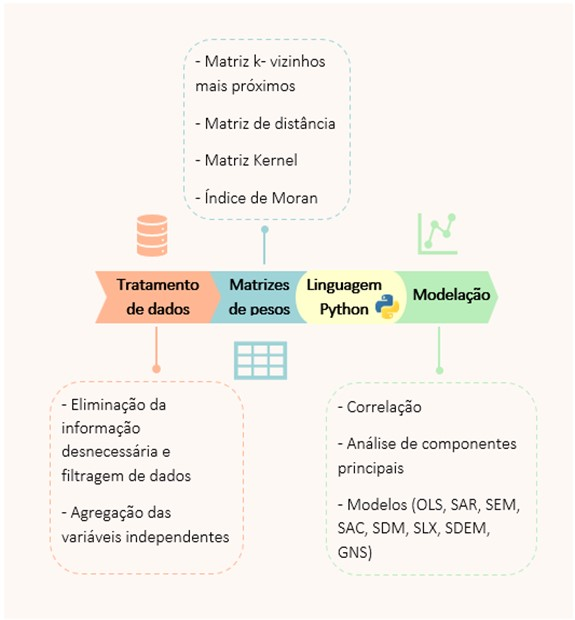
\includegraphics{C:/Users/julio/Documents/bookPoat/imagensRelatorio/figura28.jpg}
\caption{FIGURA 4: Princípios metodológicos subjacentes à análise de autocorrelação espacial - FONTE: GETIN-UA}
\end{figure}

\hypertarget{momentos-de-contacto-e-disseminauxe7uxe3o-do-projeto}{%
\subsection{\texorpdfstring{\textbf{Momentos de contacto e disseminação do projeto}}{Momentos de contacto e disseminação do projeto}}\label{momentos-de-contacto-e-disseminauxe7uxe3o-do-projeto}}

A proximidade com a autarquia de Santa Maria da Feira revelou-se essencial para a execução do projeto. Por outro lado, reunir com frequência a equipa alargada do projeto foi assumida como uma prioridade. A apresentação de peças do projeto em eventos científicos coincide, também, com momentos intercalares de divulgação dos resultados. Por último, a sessão pública de apresentação e disseminação do projeto, indicador central na candidatura, representa o culminar do projeto e dos momentos de contacto com os agentes. Seguindo a estrutura e terminologia propostas na Memória Descritiva da candidatura, apresentam-se os vários momentos correspondentes a indicadores da operação, explicitados no Anexo II.

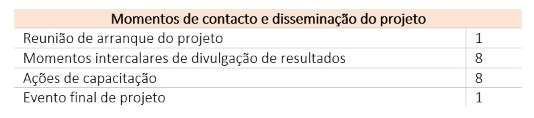
\includegraphics{C:/Users/julio/Documents/bookPoat/imagensRelatorio/figura29.jpg}

No evento final foi distribuído um inquérito de aferição de perceções e preferências, sucinto, que visava a promoção da reflexão entre/com os agentes, bem como a avaliação e enriquecimento das recomendações que vinham a ser elaboradas na fase final do projeto. Aliás, sempre que, ao longo do relatório, se mencionar a ``perceção dos agentes'', referimo-nos aos entendimentos partilhados durante o evento final de projeto, que seguiu a estrutura que se apresenta:

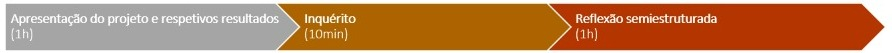
\includegraphics{C:/Users/julio/Documents/bookPoat/imagensRelatorio/figura31.jpg}

\begin{figure}
\centering
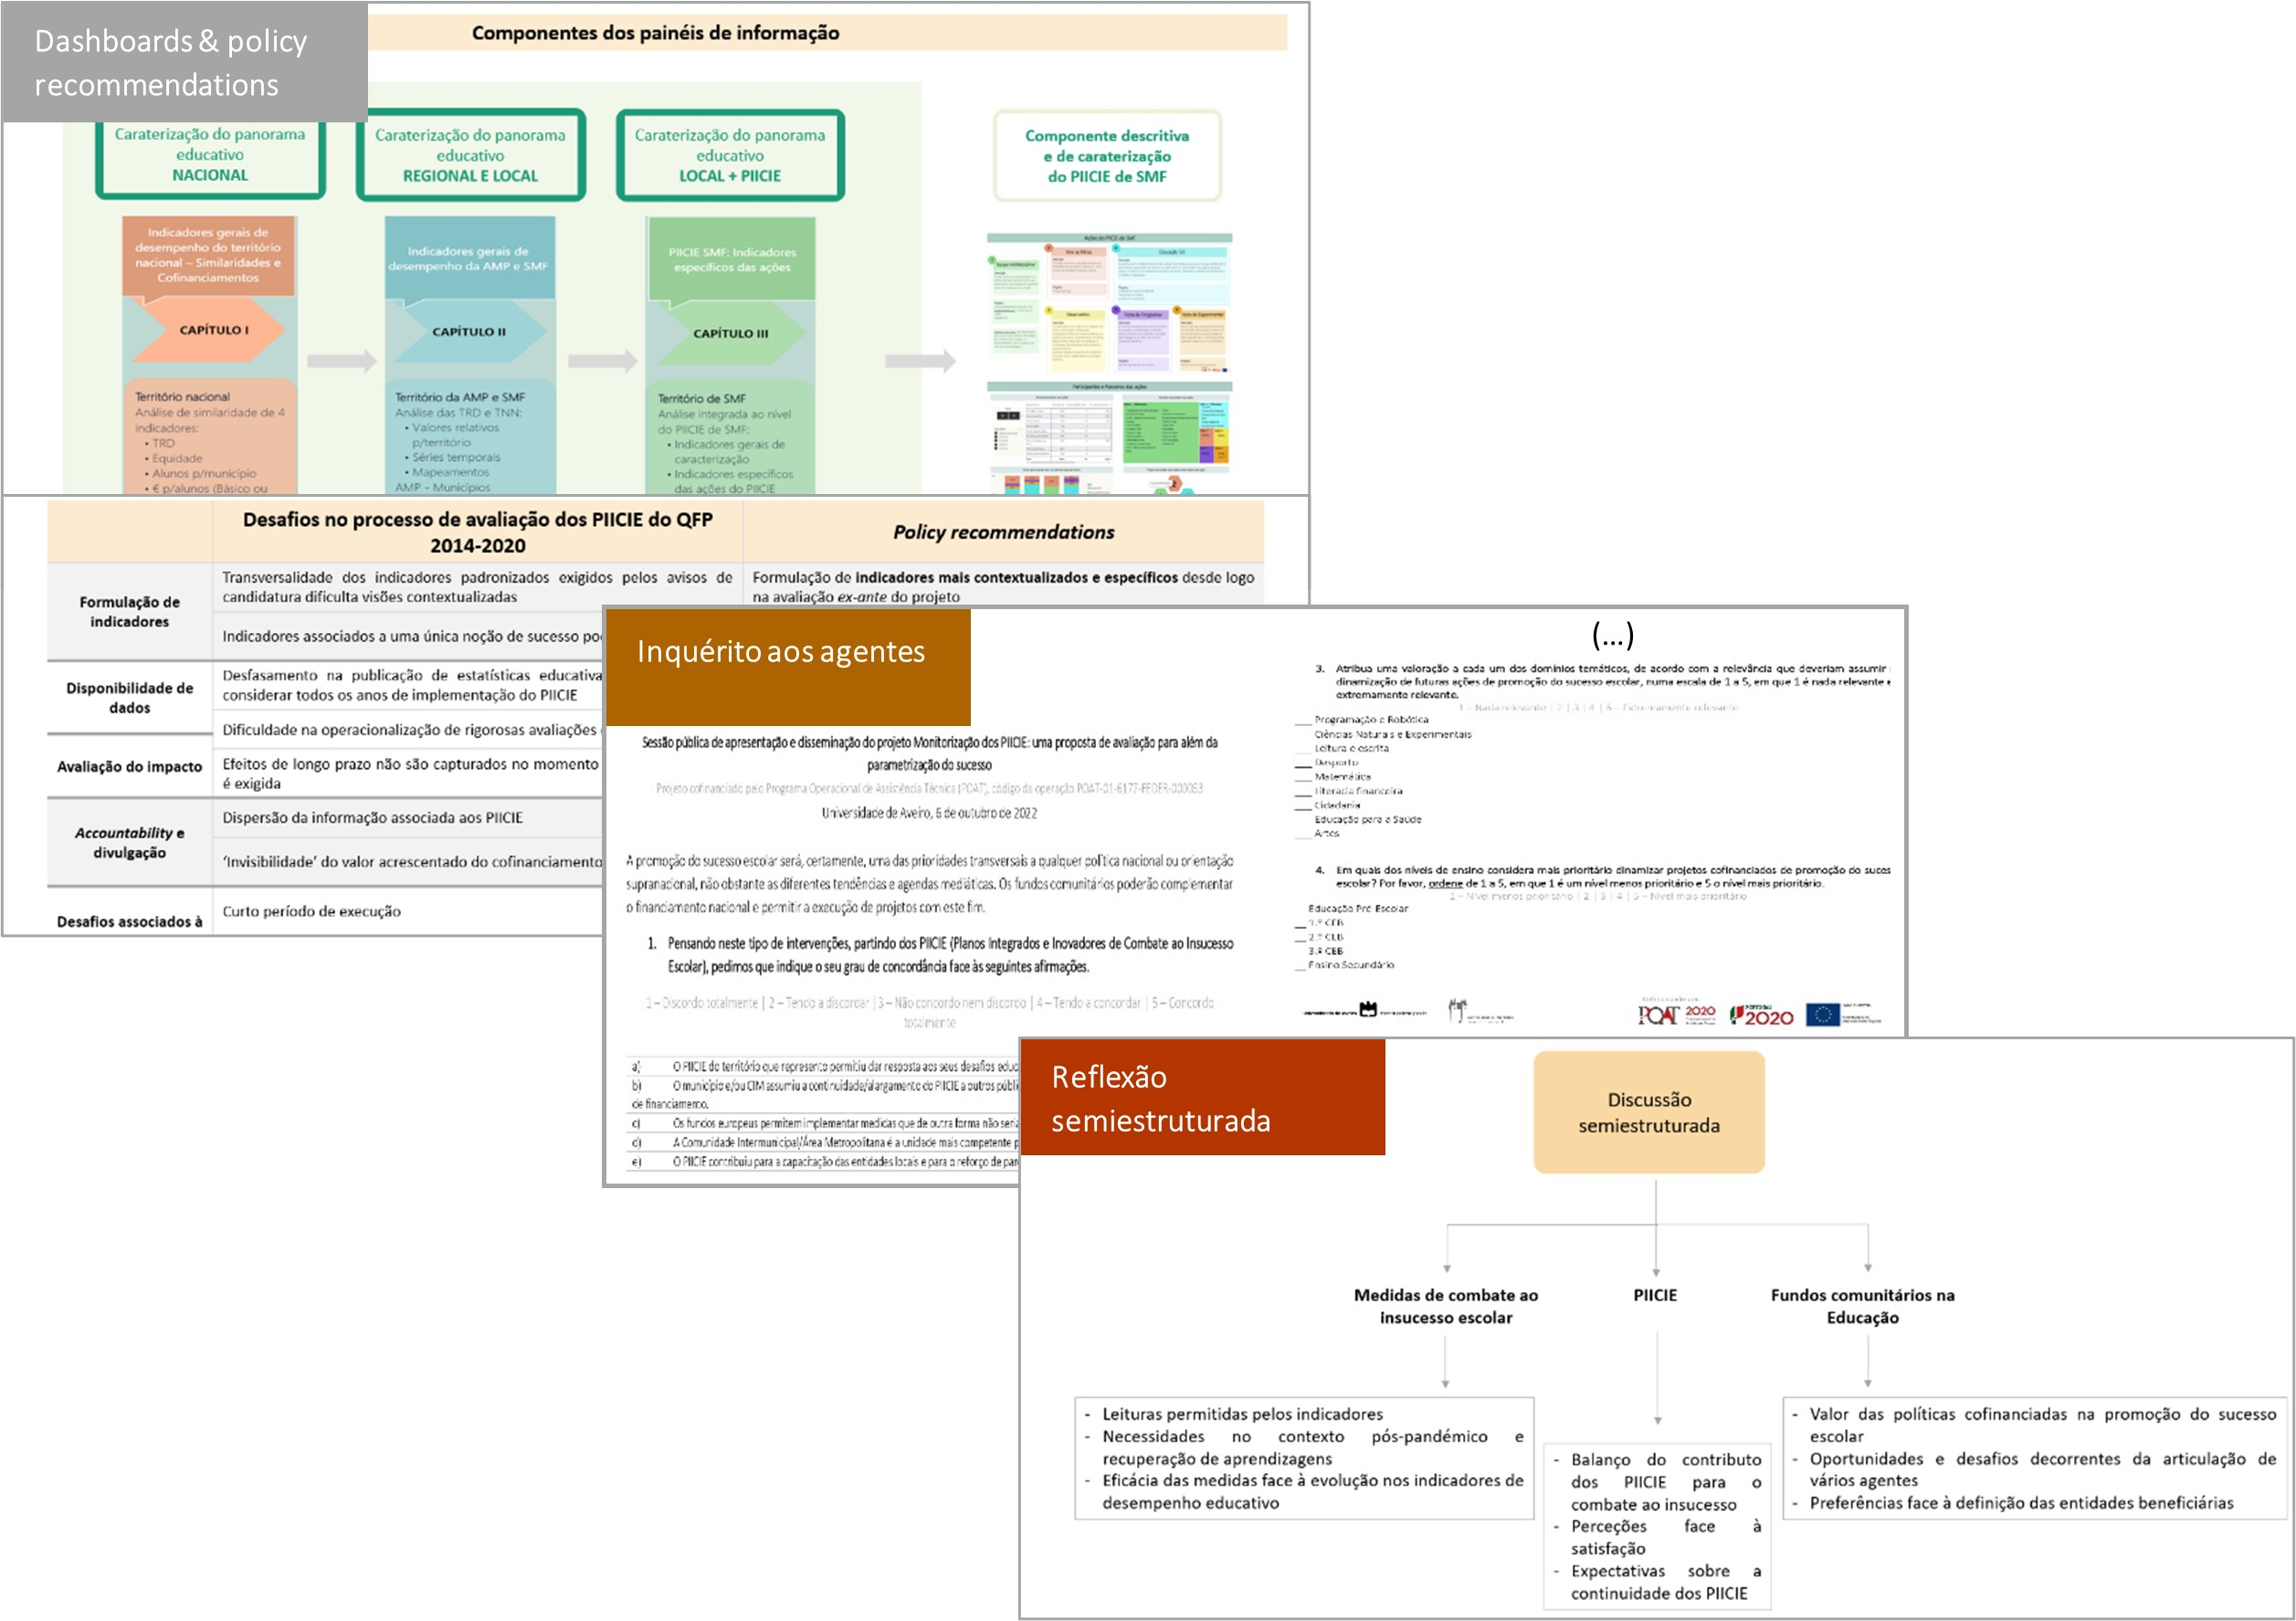
\includegraphics{C:/Users/julio/Documents/bookPoat/imagensRelatorio/figura30.jpg}
\caption{FIGURA 5: Estrutura adotada no evento final do Projeto de Monitorização dos PIICIE - peças ilustrativas - FONTE: GETIN-UA}
\end{figure}

\hypertarget{acessos-consulta-e-divulgauxe7uxe3o}{%
\subsection{\texorpdfstring{\textbf{Acessos, consulta e divulgação}}{Acessos, consulta e divulgação}}\label{acessos-consulta-e-divulgauxe7uxe3o}}

Para uma maior perceção do processo de construção dos painéis \emph{(dashboards)}, serão disponibilizados os dados originais, os \emph{scripts} em R, bem como os \emph{dataframes} utilizados, quer na modelação, quer na construção dos \emph{dashbords.} Pretende-se, assim, garantir um acesso mais completo ao `produto final' do projeto e partilhar a forma como as várias etapas deste complexo processo foram concretizadas. Adicionalmente, foi elaborado um roteiro que acompanha o projeto, com instruções que visam melhorar a experiência dos utilizadores finais.

Para aceder ao projeto final, é necessário que os utilizadores tenham instalado nos seus equipamentos informáticos o \emph{Microsoft Power BI}. Este, por sua vez, permite interagir e desenvolver novas funcionalidades de forma gratuita, mas com a limitação de não se poder compartilhar os painéis desenvolvidos no ambiente \emph{web}. Para que a partilha na internet seja possível, é necessária a aquisição da versão \emph{Power BI Pro} ou \emph{Power BI Premium}. Porém, sublinha-se que é possível aceder às funcionalidades na versão gratuita, desde que observadas as questões colocadas anteriormente. Quanto ao \emph{software R}, sendo um \emph{software} gratuito, apenas necessita de ser instalado, se os utilizadores quiserem refazer o processo de \emph{Extract, Transform, Load} (Extrair Transformar Carregar) e refazer a etapa de formação de \emph{clusters} através das técnicas de \emph{k-means}.

Importa ainda referir que o relatório final do projeto foi também desenvolvido em linguagem \emph{Markdown}, acessível no endereço eletrónico \url{https://nupec.github.io/bookPoat/}, e que a análise estatística complementar dos indicadores das TNN e TRD se encontra disponível em \url{https://rpubs.com/NUPEC/analisedescritivapoat}.

\hypertarget{monitorizauxe7uxe3o-avaliauxe7uxe3o-e-inspeuxe7uxe3o-na-poluxedtica-educativa}{%
\section{\texorpdfstring{\textbf{Monitorização, avaliação e inspeção na política educativa}}{Monitorização, avaliação e inspeção na política educativa}}\label{monitorizauxe7uxe3o-avaliauxe7uxe3o-e-inspeuxe7uxe3o-na-poluxedtica-educativa}}

As práticas de avaliação no setor da Educação não Superior têm sido mais presentes no âmbito da inspeção de escolas. O referencial, em Portugal, é detalhado e adota um olhar sobre diversas dinâmicas das escolas. À semelhança de outros Estados europeus, também Portugal segue um modelo de inspeção que não olha apenas aos resultados escolares, mas procura avaliar dinâmicas de liderança, inovação e articulação (a vários níveis, desde a articulação curricular, à articulação com a comunidade). Procura-se que os indicadores sejam contextualizados, assim aumentando o seu rigor.

Como refere Verdasca (2020), os processos de avaliação e o trabalho de inspeção `têm induzido nas escolas a introdução de práticas de monitorização, autoavaliação e melhoria escolar' (p.~120). Enquanto objetivos basilares das inspeções na educação incluem-se: definir critérios no âmbito do que se entende ser \emph{educação de qualidade} ou \emph{escola de excelência} e meios para que organizações e entidades possam atuar, como escolas e municípios (Gartner, Pant, 2011, \emph{apud} Carvalho \& Joana, 2020, p.~29); assegurar a responsabilização pública; promover melhorias e inovação ao nível das experiências e realização dos alunos; e informar o desenvolvimento de políticas e práticas educativas (The Educational Institute of Scotland (EIS), 2019, p.~3). No quadro nacional, os objetivos definidos têm evoluído, procurando integrar e responder a dinâmicas e desafios emergentes do panorama educativo. Os trabalhos de avaliação e inspeção atualmente em curso pretendem a concretização de seis objetivos principais: \emph{``1) promover a qualidade do ensino, das aprendizagens e a inclusão de todas as crianças e de todos os alunos, 2) identificar os pontos fortes e áreas prioritárias, com vista à melhoria do planeamento, gestão e ação educativa das escolas, 3) aferir a efetividade das práticas de autoavaliação das escolas, 4) promover uma cultura de participação da comunidade educativa, 5) contribuir para um melhor conhecimento público da qualidade do trabalho das escolas e 6) produzir informação para apoiar a tomada de decisão, no âmbito do desenvolvimento das políticas educativas''} (Inspeção-Geral da Educação e Ciência (IGEC), 2018a).

Diferentes países apresentam diferentes sistemas de inspeção da educação, com diferentes níveis de autonomia face ao governo central ``revelando o nível de centralização das políticas educativas de cada país e a confiança que é depositada na organização enquanto organismo responsável por garantir e promover uma educação de qualidade'' (Carvalho \& Joana, 2020, p.~27 e p.~30). O surgimento destes sistemas (com um aumento assinalável entre as décadas de 40 e 60) aconteceu, em muitos países, simultaneamente à criação e afirmação da educação pública, visando garantir iguais oportunidades a todos os cidadãos; posteriormente (na década de 80 e em diante), os sistemas inspetivos começaram a assumir crescentemente o papel de organismo de regulamentação do sistema educativo em função dos níveis de desempenho escolar dos alunos (Carvalho \& Joana, 2020, p.~29). A maioria das inspeções em educação tenderá a acontecer em escolas com financiamento público, de acordo com padrões previamente estabelecidos, promovendo uma maior \emph{accountability} (Ehren \& Shackleton, 2016, p.~299).

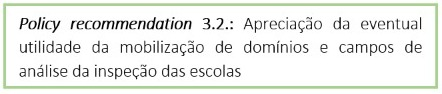
\includegraphics{C:/Users/julio/Documents/bookPoat/imagensRelatorio/figura32.jpg}

Em Portugal, importará destacar a Avaliação Integrada das Escolas realizada pela Inspeção-Geral da Educação (IGE) entre 1999 e 2002, experiência que, juntamente com outras práticas reconhecidas (e.g.~metodologia assente na aplicação de questionários proposta pela \emph{European Foundation for Quality Management} (EFQM) e projeto \emph{How Good is Our School} desenvolvido na Escócia) inspiraram o \textbf{1º ciclo nacional de avaliação externa das escolas} (Oliveira et al., 2006, p.~3). O 1º ciclo de avaliação decorreu entre 2006 e 2011 e teve na sua base um programa inovador que abrangeu a generalidade das escolas públicas do país. Entre 2012 e 2017 foi realizado o 2º ciclo de avaliação e em 2018 iniciou-se o 3º ciclo que se destaca dos anteriores dado o alargamento a escolas profissionais privadas e com contrato de associação (XXI Governo -- República Portuguesa, 2019). Uma digressão pelos quadros de referência dos três ciclos de avaliação conduzidos nas escolas em Portugal mostra uma evolução e reconfigurações ao longo do tempo, quer entre ciclos, quer entre os períodos inicial e final de cada ciclo. Através de uma análise mais aprofundada no que respeita a \textbf{domínios}, \textbf{campos de análise} e \textbf{indicadores}, depreende-se que o desenho dos quadros de referência tem sido influenciado por elementos conjunturais da governação, assim como provenientes da reflexão e investigação científica (e.g.~inclusão de indicadores de equidade no quadro de referência mais recente para avaliação de resultados académicos, recurso a indicadores que apelam e promovem o envolvimento dos diferentes agentes educativos e autonomização da autoavaliação enquanto domínio). A título ilustrativo, é apresentada, no Anexo III, a sistematização dos domínios e fatores que contribuem para a sua boa avaliação (ou campos de análise) em cada ciclo.

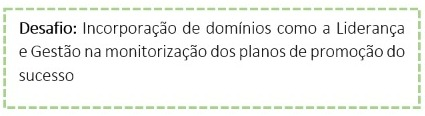
\includegraphics{C:/Users/julio/Documents/bookPoat/imagensRelatorio/figura33.jpg}

De acordo com a literatura, podem identificar-se duas tipologias ao nível dos sistemas inspetivos: uma ligada à \emph{soft governance} e outra à \emph{hard governance} (Clarke, Ozga, 2011; \emph{apud} Carvalho \& Joana, 2020, p.~31). Enquanto a primeira visa, principalmente, acompanhar e contribuir para melhorias incrementais nas organizações escolares ajustadas às suas características e necessidades (e.g.~sistema inspetivo português), a segunda tem subjacentes alguns princípios de punição e pode estar associada a modelos de inspeção escolar \emph{risk-based}, onde são privilegiadas as visitas a escolas com baixos resultados escolares (e.g.~sistema inspetivo holandês) (Carvalho \& Joana, 2020; Ehren \& Shackleton, 2016). Em inspeções soft governance existirá lugar para a avaliação de práticas e processos embora os níveis de desempenho também sejam avaliados, ao passo que nas inspeções \emph{hard governance}, essencialmente, é dada primazia à avaliação de resultados. Ainda que o sistema inspetivo português se situe no domínio da \emph{soft governance}, a execução de fundos europeus (na Educação e noutras áreas) requer um sistema de monitorização operacional com ``enorme enfoque na orientação para os resultados'' (Agência para o Desenvolvimento e Coesão, n.d.)

A definição de indicadores para avaliar as escolas em Portugal (e.g.~indicadores de alinhamento face a orientações e diretivas, indicadores processuais e de contexto e indicadores de proficiência dos alunos) (Carvalho \& Joana, 2020), assim como a publicação de relatórios com os aspetos a melhorar, têm inspirado a monitorização de possíveis fatores de influência da qualidade do sistema educativo que extravasam a esfera da escola enquanto organização. Assim, alguns dos princípios da inspeção das escolas são transferidos para as crescentes práticas de avaliação e monitorização de políticas educativas, formuladas e implementadas pelas várias escalas da governação (nacional, intermunicipal ou local), com competência para tal. Só no último ano, este esforço concretizou-se, por exemplo, nas seguintes práticas e instrumentos:

\begin{itemize}
\tightlist
\item
  \emph{Relatórios de monitorização do Plano 21\textbar23 Escola+}, no âmbito do processo de recuperação de aprendizagens em contexto (pós-)pandémico (DGEEC, 2022b);
\item
  \emph{Apoio à aprendizagem e à inclusão, 2020/2021} (DGEEC, 2022a);
\item
  \emph{Observatório de Saúde Psicológica e Bem-Estar: Monitorização e Ação} (Gaspar de Matos et al., 2022);
\item
  \emph{Recomendações no âmbito da monitorização da Carta Educativa enquanto instrumento de planeamento em educação definidas no Guião para Elaboração} (DGEEC et al., 2021).
\end{itemize}

No domínio das políticas cofinanciadas, e com o objetivo de aferir o impacto da Política de Coesão, destaca-se o relatório final de \emph{Avaliação do Contributo do PT2020 para a Promoção do Sucesso Educativo, Redução do Abandono Escolar Precoce e Empregabilidade dos Jovens} (IESE et al., 2021). As recomendações daí decorrentes giram em torno da diversificação das ofertas formativas (especialmente as profissionalizantes, procurando inverter as representações sociais negativas), promoção das iniciativas de base territorial e de proximidade, \emph{mainstreaming} de práticas bem-sucedidas, investimento digital, reforço dos Serviços de Psicologia e Orientação, formação docente e, obviamente, aposta na monitorização e avaliação.

A melhoria continua destas práticas, para além da mera atualização de informação que (em última instância) permitirá a realização de exercícios avaliativos, tem resultado de um trabalho de consolidação de abordagens e referenciais metodológicos. Acredita-se que as orientações preconizadas no âmbito do projeto \emph{How good is our School} traduzem algumas destas aspirações, com o objetivo maior de qualificar o sistema de ensino e melhorar as aprendizagens tendo por base evidências (Education Scotland, 2015, p.~8). Por exemplo, as rotinas de autoavaliação e os questionários online aos agentes educativos propostos pelo modelo escocês contribuem para informar os próprios procedimentos de inspeção (Education Scotland, 2015, pp.~9-11), permitindo funcionar como mecanismo de controlo nos ciclos avaliativos em curso (\emph{ongoing e ex-post}) e, possivelmente, como componente de avaliação \emph{ex-ante} em ciclos de inspeção futuros.

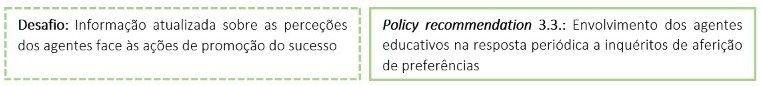
\includegraphics{C:/Users/julio/Documents/bookPoat/imagensRelatorio/figura34.jpg}

No que respeita à avaliação de impactos, quer ao nível deste tipo de práticas, quer de outras medidas de monitorização e avaliação, importará sublinhar que mudanças estruturais que conduzam à melhoria de níveis de desempenho levam o seu tempo (geralmente entre 5 a 10 anos) (van den Berg e Vandenberghe, 1981; Stringfield, 2002; Visscher, 2002; \emph{apud} Ehren \& Shackleton, 2016, p.~318). Por outro lado, impactos que contribuam para melhorias da qualidade dos sistemas de ensino e das aprendizagens tenderão a ser mais positivos se resultarem de alterações na cultura organizacional comparativamente a meras imposições externas (Ehren et al., 2015, \emph{apud} Carvalho \& Joana, 2020, p.~38). Ao nível da política cofinanciada em análise, considera-se ainda essencial sublinhar ``que o alcance dos objetivos e a produção dos resultados desejáveis dos PIICIE surge muito dependente das condições para dar continuidade aos projetos, quer seja porque a própria natureza dos Planos exige mais tempo útil para a produção de resultados (mais do que os 3 anos previstos), quer porque a concretização dos Planos no terreno foi tardia (\ldots)'' (IESE et al., 2021, p.~46).

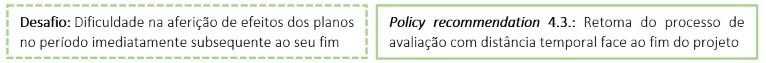
\includegraphics{C:/Users/julio/Documents/bookPoat/imagensRelatorio/figura35.jpg}

\hypertarget{enquadramento-e-contexto-do-objeto-de-estudo}{%
\chapter{\texorpdfstring{\textbf{Enquadramento e contexto do objeto de estudo}}{Enquadramento e contexto do objeto de estudo}}\label{enquadramento-e-contexto-do-objeto-de-estudo}}

Aquando da candidatura do presente projeto, o objeto de estudo delimitado foi o PIICIE enquanto operação cofinanciada, mas não havia ainda sido selecionado(s) caso(s) de estudo. Foram vários os motivos que presidiram à definição dos PIICIE como objeto de estudo, vários deles reforçados pelas orientações e quadros estratégicos, entretanto emanados das instituições europeias e nacionais. Destacam-se os seguintes motivos:

\begin{itemize}
\tightlist
\item
  A inovação do quadro de governação dos PIICIE, sendo a única operação enquadrada no Objetivo Temático 10, do quadro 2014-2020, que pode ter como entidades beneficiárias as Comunidades Intermunicipais;
\item
  A constatação de uma melhoria expressiva de Portugal nos indicadores de desempenho educativo medidos a nível europeu, designadamente no abandono escolar precoce;
\item
  A renovação dos objetivos de promoção do sucesso no QFP 2021-2027, especialmente perante a necessidade de recuperação de aprendizagens.
\end{itemize}

Cedo se percebeu, no arranque do projeto, que a informação aberta disponível seria insuficiente para se encetar uma verdadeira avaliação de vários PIICIE, pelo que se agudizou a necessidade de seleção de casos de estudo. Após contactos com outros Municípios e Comunidades Intermunicipais, ao longo do mês de dezembro de 2021, optou-se por estabelecer uma parceria com Santa Maria da Feira. Desta forma, foi possível enveredar por um caminho de exploração minuciosa de um PIICIE, em estreita articulação com a autarquia (cenário que seria improvável perante vários casos de estudo). O objetivo não passa pela generalização, mas por uma especialização que permite afirmações claras e objetivas, confrontando as informações e perceções, sempre que possível, com outros PIICIE que tenham informação disponível, ainda que amiúde de forma implícita.

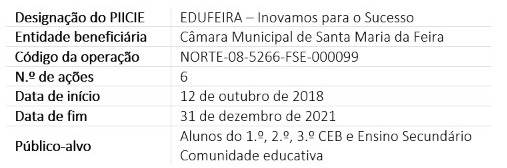
\includegraphics{C:/Users/julio/Documents/bookPoat/imagensRelatorio/figura36.jpg}

Focando, então, no caso de estudo, o PIICIE de Santa Maria da Feira surge em resposta aos avisos de candidatura NORTE-66-2016-28 e NORTE-66-2016-29. Recorrendo ao jargão europeu, na sequência desta candidatura foi financiada uma única operação que, por sua vez, se desdobra em várias ações. Por oposição, há outras entidades beneficiárias que gerem um PIICIE cujas ações correspondem a diferentes operações cofinanciadas.

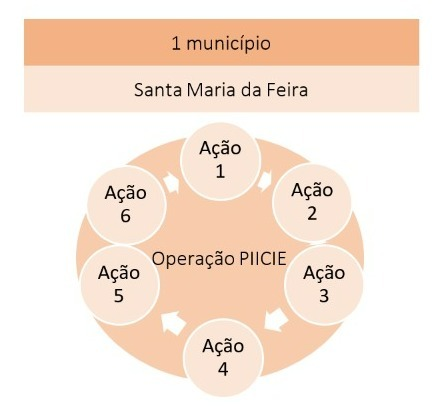
\includegraphics{C:/Users/julio/Documents/bookPoat/imagensRelatorio/figura2.jpg}

Em Santa Maria da Feira, cada uma das 6 ações compreendidas na operação cumpre um propósito distinto e enquadra-se em diferentes domínios temáticos. Esta diversidade deve ser tida em conta aquando da formulação de indicadores que combinem a transversalidade com a especificidade. Dentro de cada ação são, ainda, dinamizados diferentes projetos e medidas que visem a melhoria do sucesso escolar.

Cada uma das ações do PIICIE de Santa Maria da Feira pode ser resumida através de uma palavra ou expressão, algumas remetendo para os princípios subjacentes, outras para os domínios temáticos:

\begin{figure}
\centering
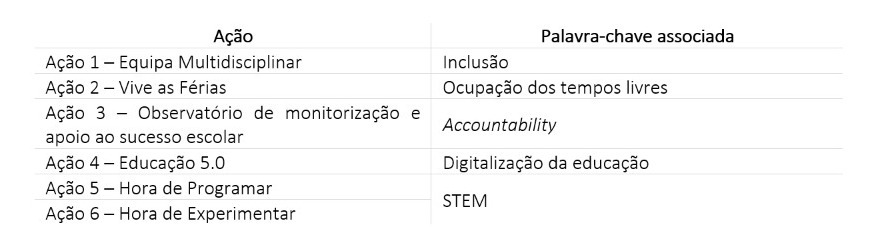
\includegraphics{C:/Users/julio/Documents/bookPoat/imagensRelatorio/figura4.jpg}
\caption{FIGURA 6: Ações (6) cofinanciadas no âmbito do PIICIE do Município de Santa Maria da Feira - FONTE: GETIN-UA -- Informação documental facultada pelo município de SMF}
\end{figure}

Por outro lado, há ações que têm uma abrangência de público declaradamente alargada, como a Ação 2 -- Vive as Férias ou, no limite, a Ação 3 -- Observatório, cuja plataforma de consulta pública deveria ser visitada por todos os munícipes que assim desejassem. Por outro lado, a Ação 1 -- Equipa Multidisciplinar compreende um rigoroso processo de seleção dos alunos a incluir nas atividades; a Ação 6 -- Hora de Experimentar destina-se a alunos de apenas 4 dos 9 Agrupamentos de Escolas\footnote{Sublinhe-se, desde já, que a Hora de Experimentar foi alargada aos restantes Agrupamentos de Escolas, ainda que sem cofinanciamento europeu, sendo as despesas assumidas pela autarquia.}. Ficam fora desta análise as ações do PIICIE intermunicipal, promovido pela Área Metropolitana do Porto.

\hypertarget{diagnuxf3stico-do-sucesso-escolar-no-territuxf3rio-de-estudo}{%
\chapter{\texorpdfstring{\textbf{Diagnóstico do sucesso escolar no território de estudo}}{Diagnóstico do sucesso escolar no território de estudo}}\label{diagnuxf3stico-do-sucesso-escolar-no-territuxf3rio-de-estudo}}

Um dos principais objetivos da avaliação na educação passará por reunir evidências ou informação de apoio à decisão no desenvolvimento das próprias políticas educativas, com a expectativa de fornecer contributos valiosos aos agentes educativos no caminho da melhoria de processos e desempenhos e, consequentemente, elevar a qualidade do sistema de ensino.

As opções analíticas seguem pressupostos que têm sido amplamente debatidos ao nível da investigação científica e aplicada na territorialização de políticas públicas, nomeadamente as políticas de educação, pelo que se assume essencial ter um diagnóstico das principais tendências e padrões das dinâmicas em análise -- o insucesso escolar (Ioannidou, 2010; Marques et al., 2020; Santos et al., 2019).

\hypertarget{cofinanciamentos-na-promouxe7uxe3o-do-sucesso}{%
\section{\texorpdfstring{\textbf{Cofinanciamentos na promoção do sucesso}}{Cofinanciamentos na promoção do sucesso}}\label{cofinanciamentos-na-promouxe7uxe3o-do-sucesso}}

O domínio do Capital Humano (expressão que reflete o espírito da Estratégia de Lisboa, de 2020) foi operacionalizado pelas operações cofinanciadas enquadradas pelo Objetivo Temático (OT) 10 (Investir no ensino, nas competências e na aprendizagem ao longo da vida) do quadro financeiro plurianual 2014-2020, por sua vez desdobrado em cinco prioridades de investimento (PI). A prioridade 10.1\footnote{Redução do abandono escolar precoce e promoção da igualdade de acesso a educação pré-escolar, ensino básico e secundário de boa qualidade, incluindo percursos de aprendizagem formais e não-formais para reintegração no ensino e na formação.} é aquela mais diretamente voltada para a promoção do sucesso escolar e da igualdade de oportunidades, no âmbito da qual se enquadram os PIICIE, candidatados através dos Programas Operacionais Regionais (POR), ao invés do Programa Operacional Capital Humano (POCH).

Olhando apenas aos POR, à data de 31 de março de 2022, \textbf{os PIICIE eram a tipologia de operações dominante, em número de operações, na prioridade 10.1 nas regiões Norte e Alentejo}. Por outro lado, no que às prioridades de investimento diz respeito, e também em número de operações nos POR, a PI 10.1 é a segunda mais dominante na região Norte e a primeira no Algarve. A PI 10.5, associada aos equipamentos educativos, e a única cofinanciada pelo Fundo Europeu de Desenvolvimento Regional (FEDER), acaba por ter maior destaque nas regiões do Continente, por via dos problemas infraestruturais de várias instituições.

\begin{figure}
\centering
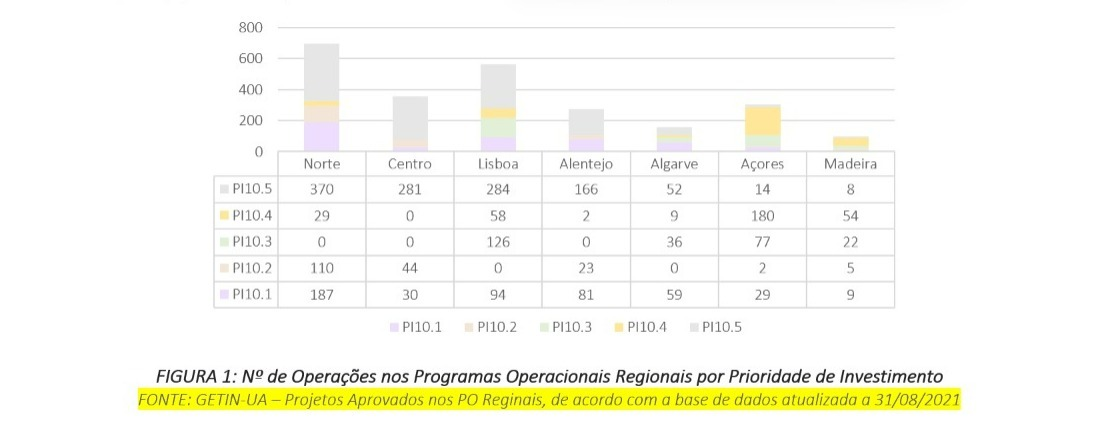
\includegraphics{C:/Users/julio/Documents/bookPoat/imagensRelatorio/figura6.jpg}
\caption{FIGURA 7: Nº de Operações nos Programas Operacionais Regionais por Prioridade de Investimento - FONTE: GETIN-UA -- Projetos Aprovados nos PO Reginais, de acordo com a base de dados atualizada a 31/08/2021}
\end{figure}

Olhando ao caso de estudo de Santa Maria da Feira, também a PI10.5 mobiliza um maior montante de fundo total aprovado, quando olhando apenas ao cofinanciamento enquadrado pelo POR Norte. Esta realidade feirense não se encontra totalmente alinhada com a tendência da AMP (não como entidade beneficiária, mas como unidade territorial), uma vez que, no que diz respeito ao financiamento enquadrado pelo POR Norte, a PI 10.2 (orientada para o Ensino Superior) acaba por ser mais dominante do que a PI 10.1.

\begin{figure}
\centering
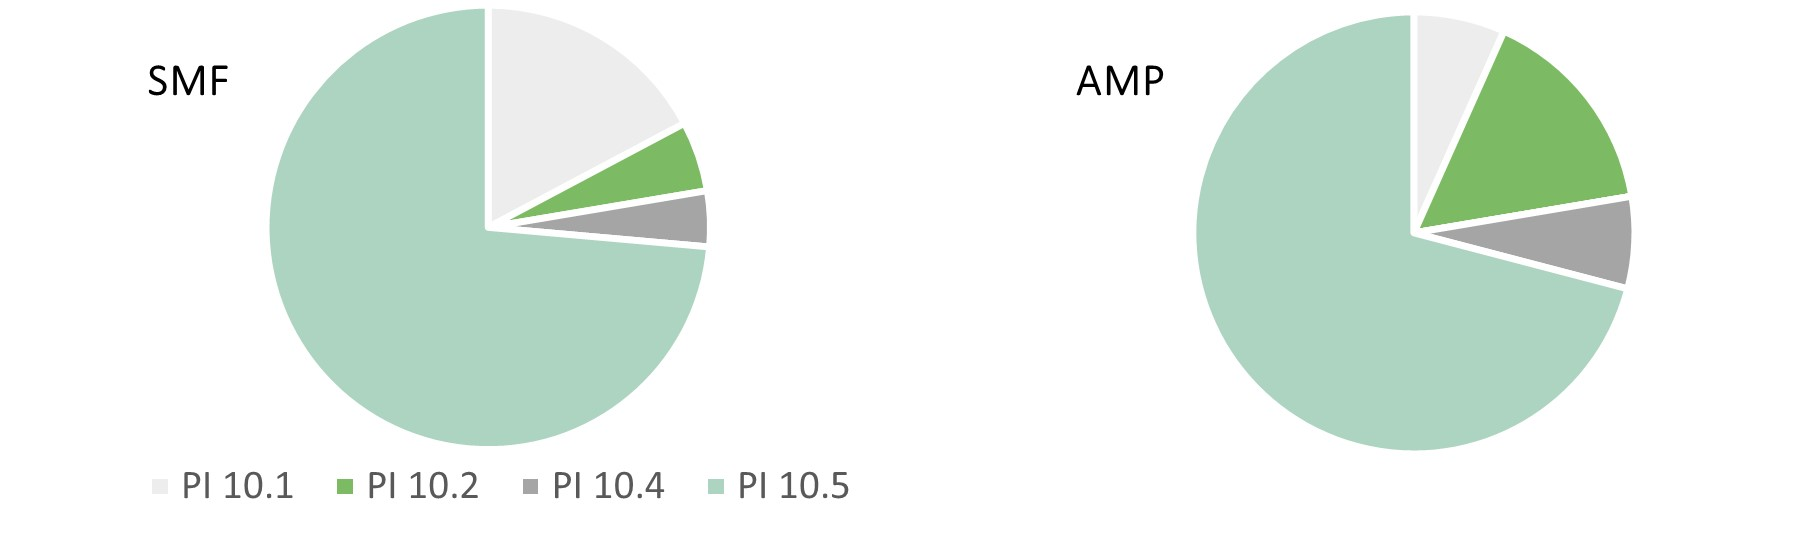
\includegraphics{C:/Users/julio/Documents/bookPoat/imagensRelatorio/figura7.jpg}
\caption{FIGURA 8: Distribuição do fundo total aprovado, por PI do OT10, para Santa Maria da Feira e AMP no QFP 2014-2020, POR Norte - FONTE: GETIN-UA -- Projetos Aprovados do PO Norte, de acordo com a base de dados atualizada a 31/08/2021}
\end{figure}

Nos cofinanciamentos por via do POCH, as tendências são semelhantes no território do município de estudo (Santa Maria da Feira) e da respetiva NUTS III (AMP). Ao nível deste programa de financiamento, ganha maior destaque a PI 10.4, evidenciando a relevância da formação profissional no território.\footnote{Para consulta das operações aprovadas, consultar o Anexo IV.
  Importa sublinhar que, embora tematicamente semelhantes, as Prioridades de Investimento (PI) apresentam diferenças ao nível dos PO Regionais e do POCH.}

\begin{figure}
\centering
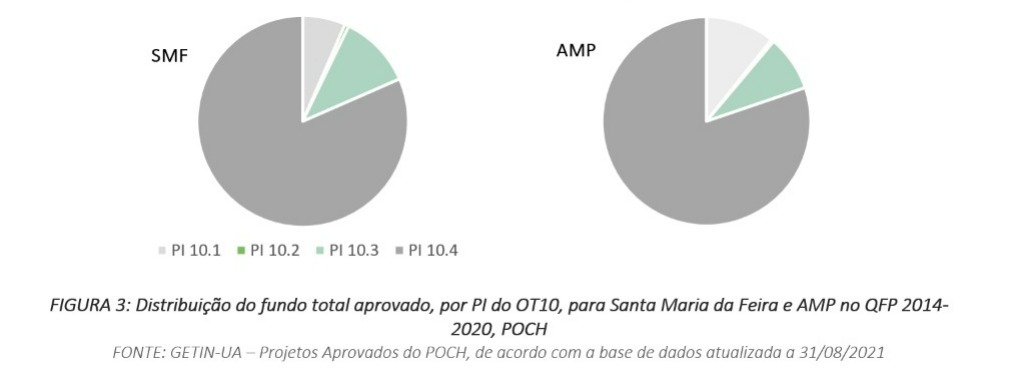
\includegraphics{C:/Users/julio/Documents/bookPoat/imagensRelatorio/figura8.jpg}
\caption{FIGURA 9: Distribuição do fundo total aprovado, por PI do OT10, para Santa Maria da Feira e AMP no QFP 2014-2020, POCH - FONTE: GETIN-UA -- Projetos Aprovados do POCH, de acordo com a base de dados atualizada a 31/08/2021}
\end{figure}

No âmbito do POR Norte, o cofinanciamento destinado a entidades de Santa Maria da Feira (4 378 284,80€) totaliza 3\% do montante total da AMP (143 160 673,82€), enquanto no contexto do POCH esta proporção é de 4\% (volume de 23 202 113,43€ mobilizado por Santa Maria da Feira no total da AMP que ascende a 619 559 890,53€).

Voltando ao contexto dos \textbf{PIICIE}, permita-se reiterar dois pontos: i) o seu peculiar modelo de governação, uma vez que estes são a \textbf{única operação cofinanciada do OT 10 em que as comunidades intermunicipais podem ser entidades beneficiárias} (tal como os municípios e, em excecionais casos, Agrupamentos de Escolas e até centros de formação), no âmbito dos Pactos para o Desenvolvimento e Coesão Territorial (PDCT); e ii) a clara aposta da região Norte nesta tipologia de operação cofinanciada. As operações implementadas na Região Norte têm uma taxa de cofinanciamento até 85\%\footnote{Consultar Anexo V.}.

Seguidamente, é apresentado um dos painéis integrados no capítulo I, de caracterização do panorama educativo nacional, que visa ilustrar a distribuição do investimento ao nível dos programas PIICIE nos diferentes territórios de Portugal Continental. Este painel permite a leitura espacializada dos valores do cofinanciamento em duas dimensões -- à escala das NUTSIII e à escala dos municípios, as duas tipologias de entidades beneficiárias do programa. De acordo com a informação de base que foi utilizada, atualizada até agosto de 2021, e que inclui valores do fundo aprovado de operações PIICIE entre 2016 e 2020, observa-se que o total de recursos atribuídos a comunidades intermunicipais perfaz 46,98 milhões de euros (M/€), enquanto a verba destinada aos 131 municípios beneficiários totaliza 52,41 M/€.

No gráfico da esquerda, integrado no painel do cofinanciamento, é possível percorrer os valores atribuídos às duas tipologias de entidades beneficiárias dos programas PIICIE, separada e cumulativamente. Estes valores, por sua vez, foram espacializados a partir do rácio entre os recursos alocados e a população de crianças e jovens a frequentar os diferentes níveis de ensino em 2019/20, com o objetivo de melhor analisar comparativamente a distribuição do cofinanciamento atendendo ao público-alvo do programa. Os mapas apresentam assim as distribuições dos recursos para três níveis -- a educação pré-escolar, o ensino básico e o ensino secundário -- permitindo uma aproximação aos grupos etários de população residente que podem beneficiar da implementação dos programas PIICIE. Importa sublinhar que não foi possível aferir a que público concreto cada PIICIE (intermunicipal ou municipal) pretendia dar respostas, pelo que os valores apresentados refletem uma visão geral do indicador. A acompanhar cada mapa, tabelas descritivas permitem a consulta dos valores por município -- valores reais quando se analisa o fundo total aprovado real por município beneficiário e valores estimados quando o olhar recai sobre o valor extrapolado da divisão da verba atribuída a cada entidade intermunicipal beneficiária pelo número de municípios que dela fazem parte.

O critério utilizado na criação dos mapas foi o dos quartis -- Q1, Q2, Q3 e Q4 -- numa escala crescente. Territórios do mapa no Q1 mostram os municípios que terão recebido menos recursos de forma proporcional ao número de crianças e jovens a frequentar desde a educação pré-escolar ao ensino secundário, enquanto no Q4 estão aqueles com maior volume de cofinanciamento. O município de SMF está no Q4, nos três níveis.

\begin{figure}
\centering
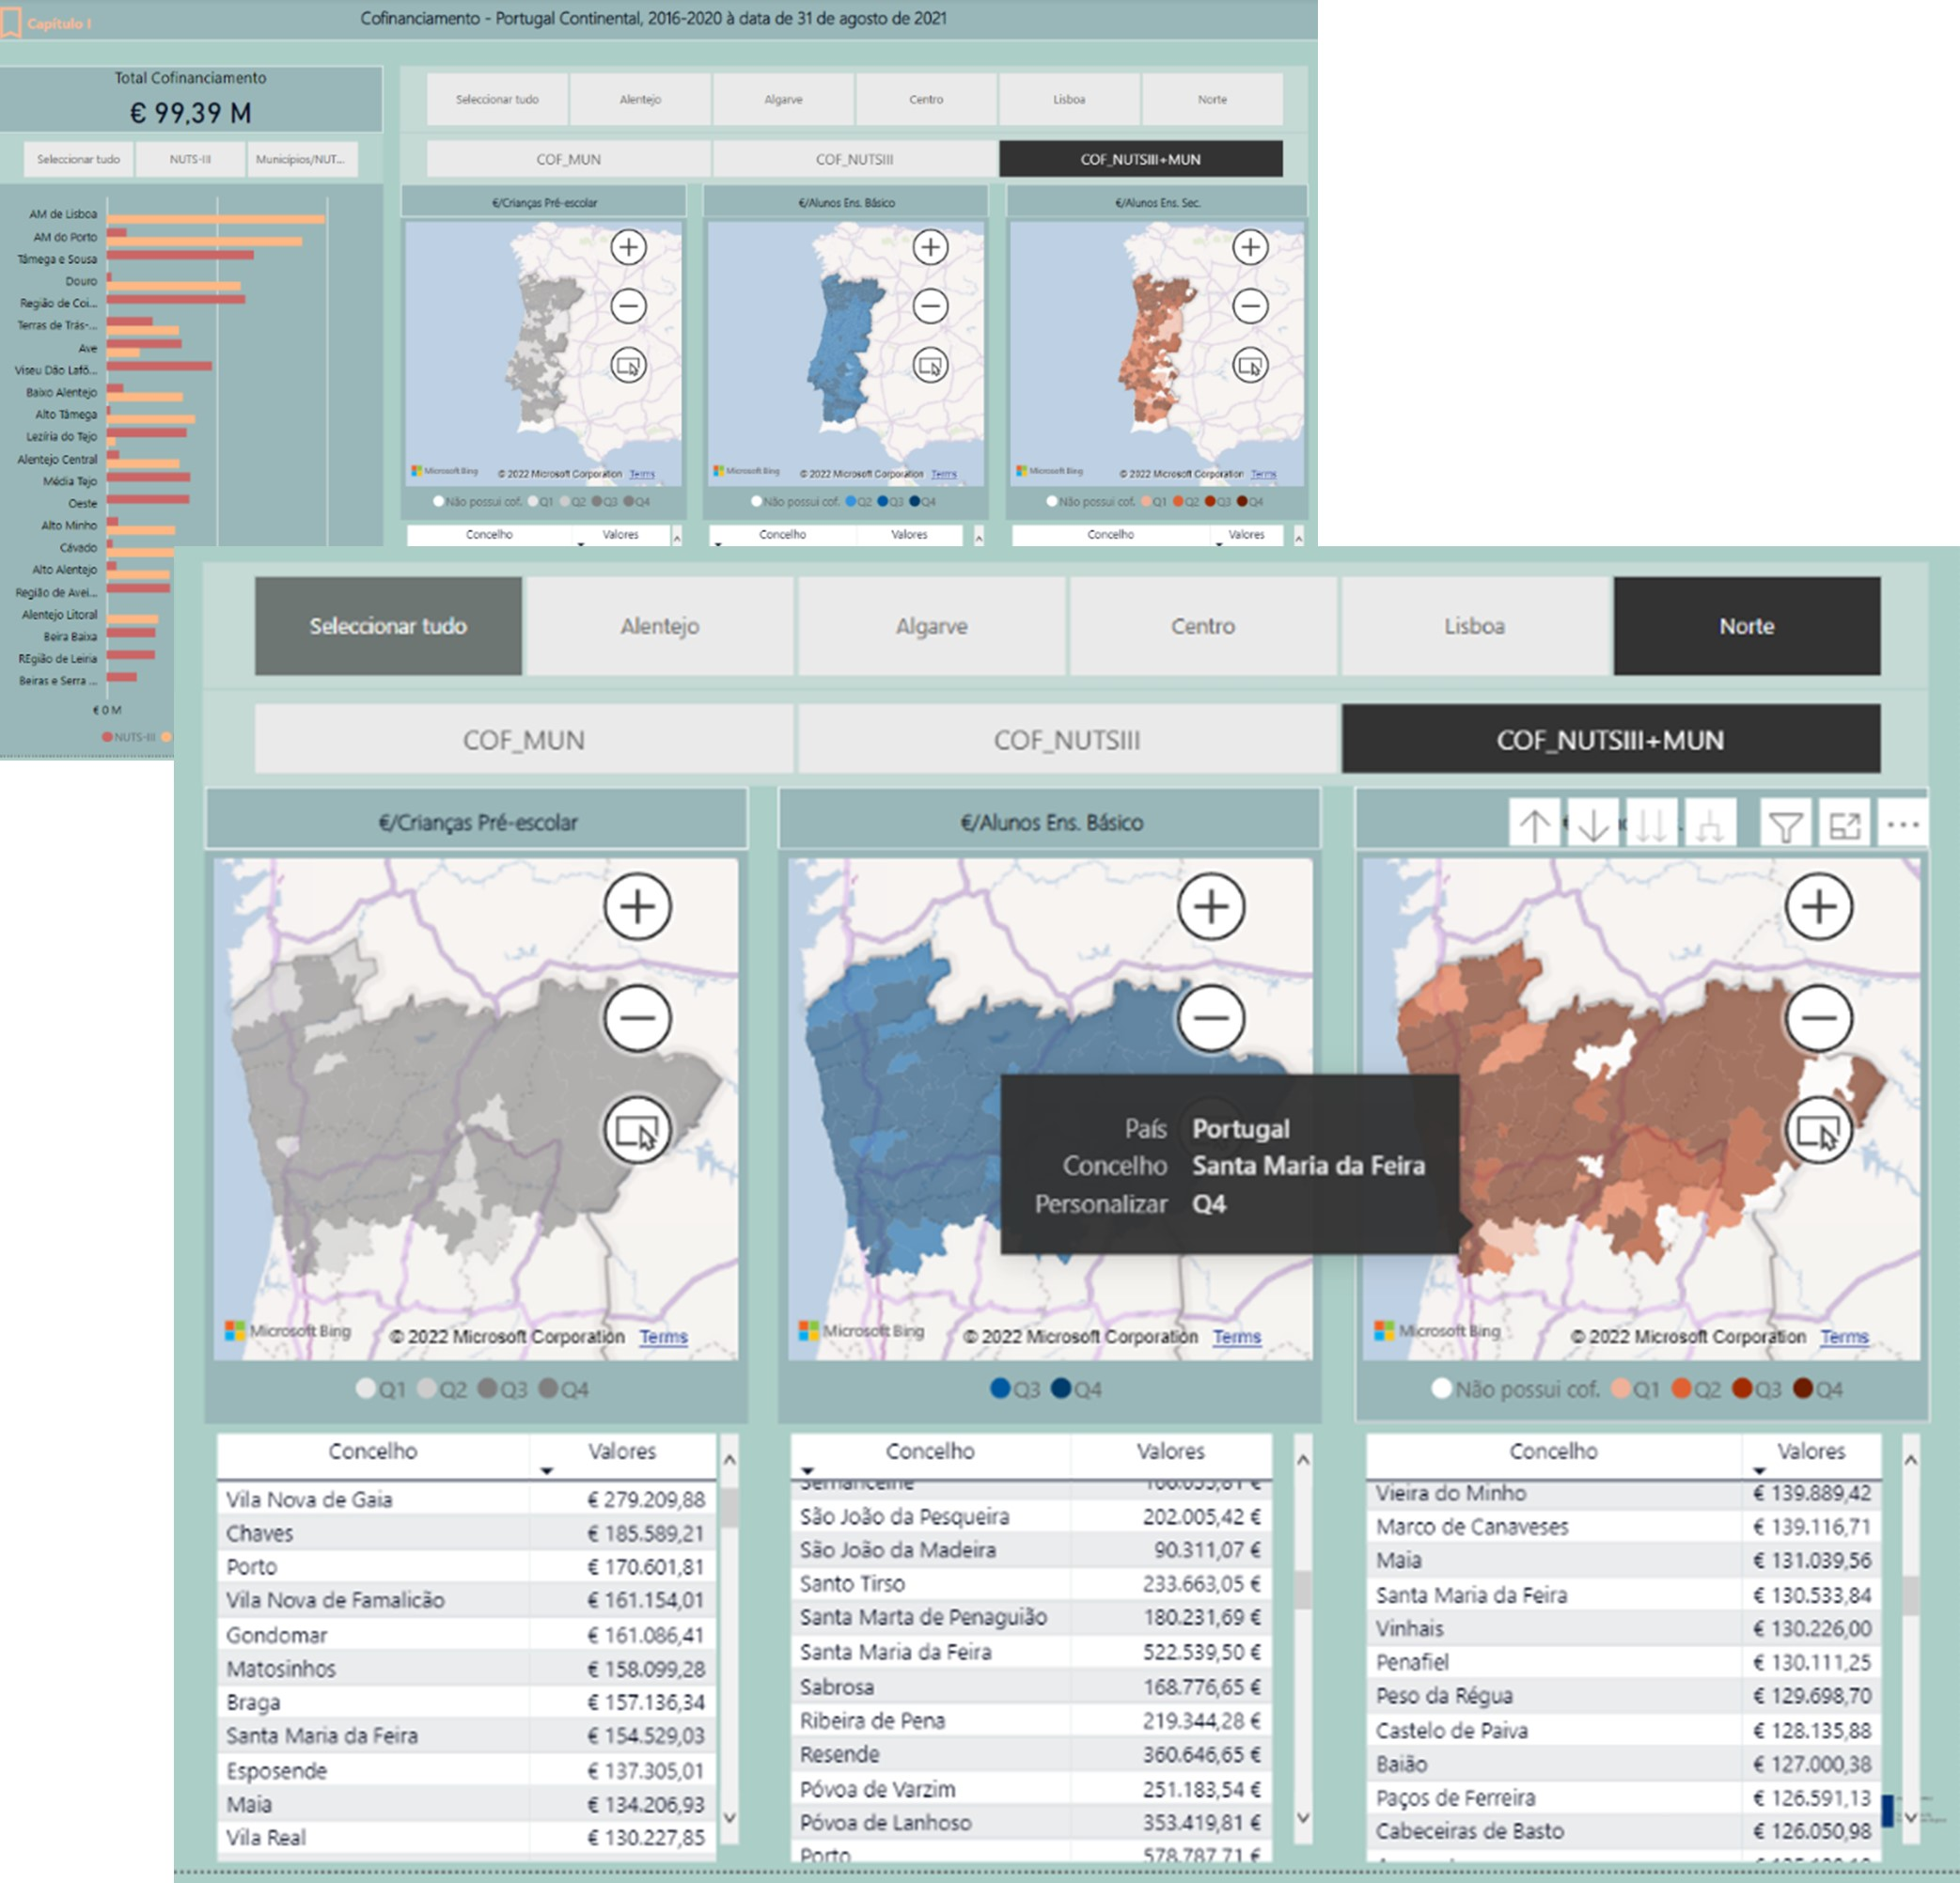
\includegraphics{C:/Users/julio/Documents/bookPoat/imagensRelatorio/figura37.jpg}
\caption{FIGURA 10: Capítulo I -- Caracterização do panorama educativo nacional: Painel do Mapeamento do cofinanciamento dos PIICIE, Portugal Continental e Região Norte, 2016-2020 - FONTE: GETIN-UA}
\end{figure}

\hypertarget{tenduxeancias-e-padruxf5es}{%
\section{\texorpdfstring{\textbf{Tendências e padrões}}{Tendências e padrões}}\label{tenduxeancias-e-padruxf5es}}

As evidências reunidas, dada a informação desagregada à qual foi possível aceder, partem de uma análise geral a nível nacional para depois se centrarem nas regiões de referência do município de estudo. Encontram-se estruturadas em dois pontos: 1) uma análise de similaridades entre municípios (\emph{clusters} territoriais) cruzando indicadores de caracterização socioeducativa, de cofinanciamento e de desempenho e 2) uma análise estatística dos indicadores gerais de resultado indicados no aviso de candidatura dos PIICIE (TRD e TNN).

Ao nível da análise de similaridades, que utiliza a técnica de \emph{k-means}, a criação dos \emph{clusters} deu-se a partir da composição de dois conjuntos de variáveis, onde o primeiro conjunto incluiu o total de alunos, a TRD e o indicador de equidade e o segundo conjunto permuta o total de alunos pelo indicador de cofinanciamento. A análise de similaridades pode ser aplicada aos ensinos básico e secundário, como referido no ponto da metodologia, e o respetivo painel permite a análise espácio-temporal para \textbf{dois, três ou quatros \emph{clusters} }, onde a formação dos \emph{clusters} se dá a partir de valores médios dos 278 concelhos de Portugal Continental.

A figura seguinte destaca a área abrangida pelos 17 concelhos da AMP. Do conjunto de dados que é possível explorar, importa destacar o valor acrescentado deste tipo de painéis na visualização da informação efetivamente relevante de forma integrada -- neste caso associada ao (in)sucesso escolar. As opções selecionadas para a representação dos dados (e.g.~tabelas com os valores específicos das variáveis, gráficos que traduzem a evolução dessas variáveis numa série temporal e espacialização das variáveis) concorrem para uma análise mais completa de caracterização dos próprios \emph{clusters}.

A título ilustrativo, a análise de similaridades dos dados abaixo apresentados, relativos ao ano letivo de 2019/2020 e ao ensino básico agregado (1ºCEB + 2ºCEB + 3ºCEB), mostra que:

\begin{itemize}
\item
  \begin{enumerate}
  \def\labelenumi{\roman{enumi})}
  \tightlist
  \item
    Na agregação que considera o total de alunos, a TRD e a equidade \textbf{\emph{(similaridade 1)}} , as similaridades intragrupos de concelhos da AMP (por referência aos valores médios nacionais das variáveis usadas) indiciam que em territórios com número de alunos mais baixo o indicador de equidade tende a ser mais alto e as TDR mais baixas (e.g.~\emph{clusters} 3 e 1), verificando-se também o inverso (e.g.~\emph{cluster} 4). O município de SMF surge integrado no \textbf{\emph{cluster 3}} em 2019/20;
  \end{enumerate}
\item
  \begin{enumerate}
  \def\labelenumi{\roman{enumi})}
  \setcounter{enumi}{1}
  \tightlist
  \item
    Já na agregação que considera o indicador de cofinanciamento, a TRD e a equidade \textbf{\emph{(similaridade 2)}}, percebe-se que o \emph{cluster} 1, onde a TRD é alta e os níveis de cofinanciamento e a equidade são baixos, se distancia bastante dos restantes grupos. Aqui SMF surge no \textbf{\emph{cluster 4}}, conjunto formado por municípios com equidade e cofinanciamento altos e baixas/médias TRD.
  \end{enumerate}
\end{itemize}

\begin{figure}
\centering
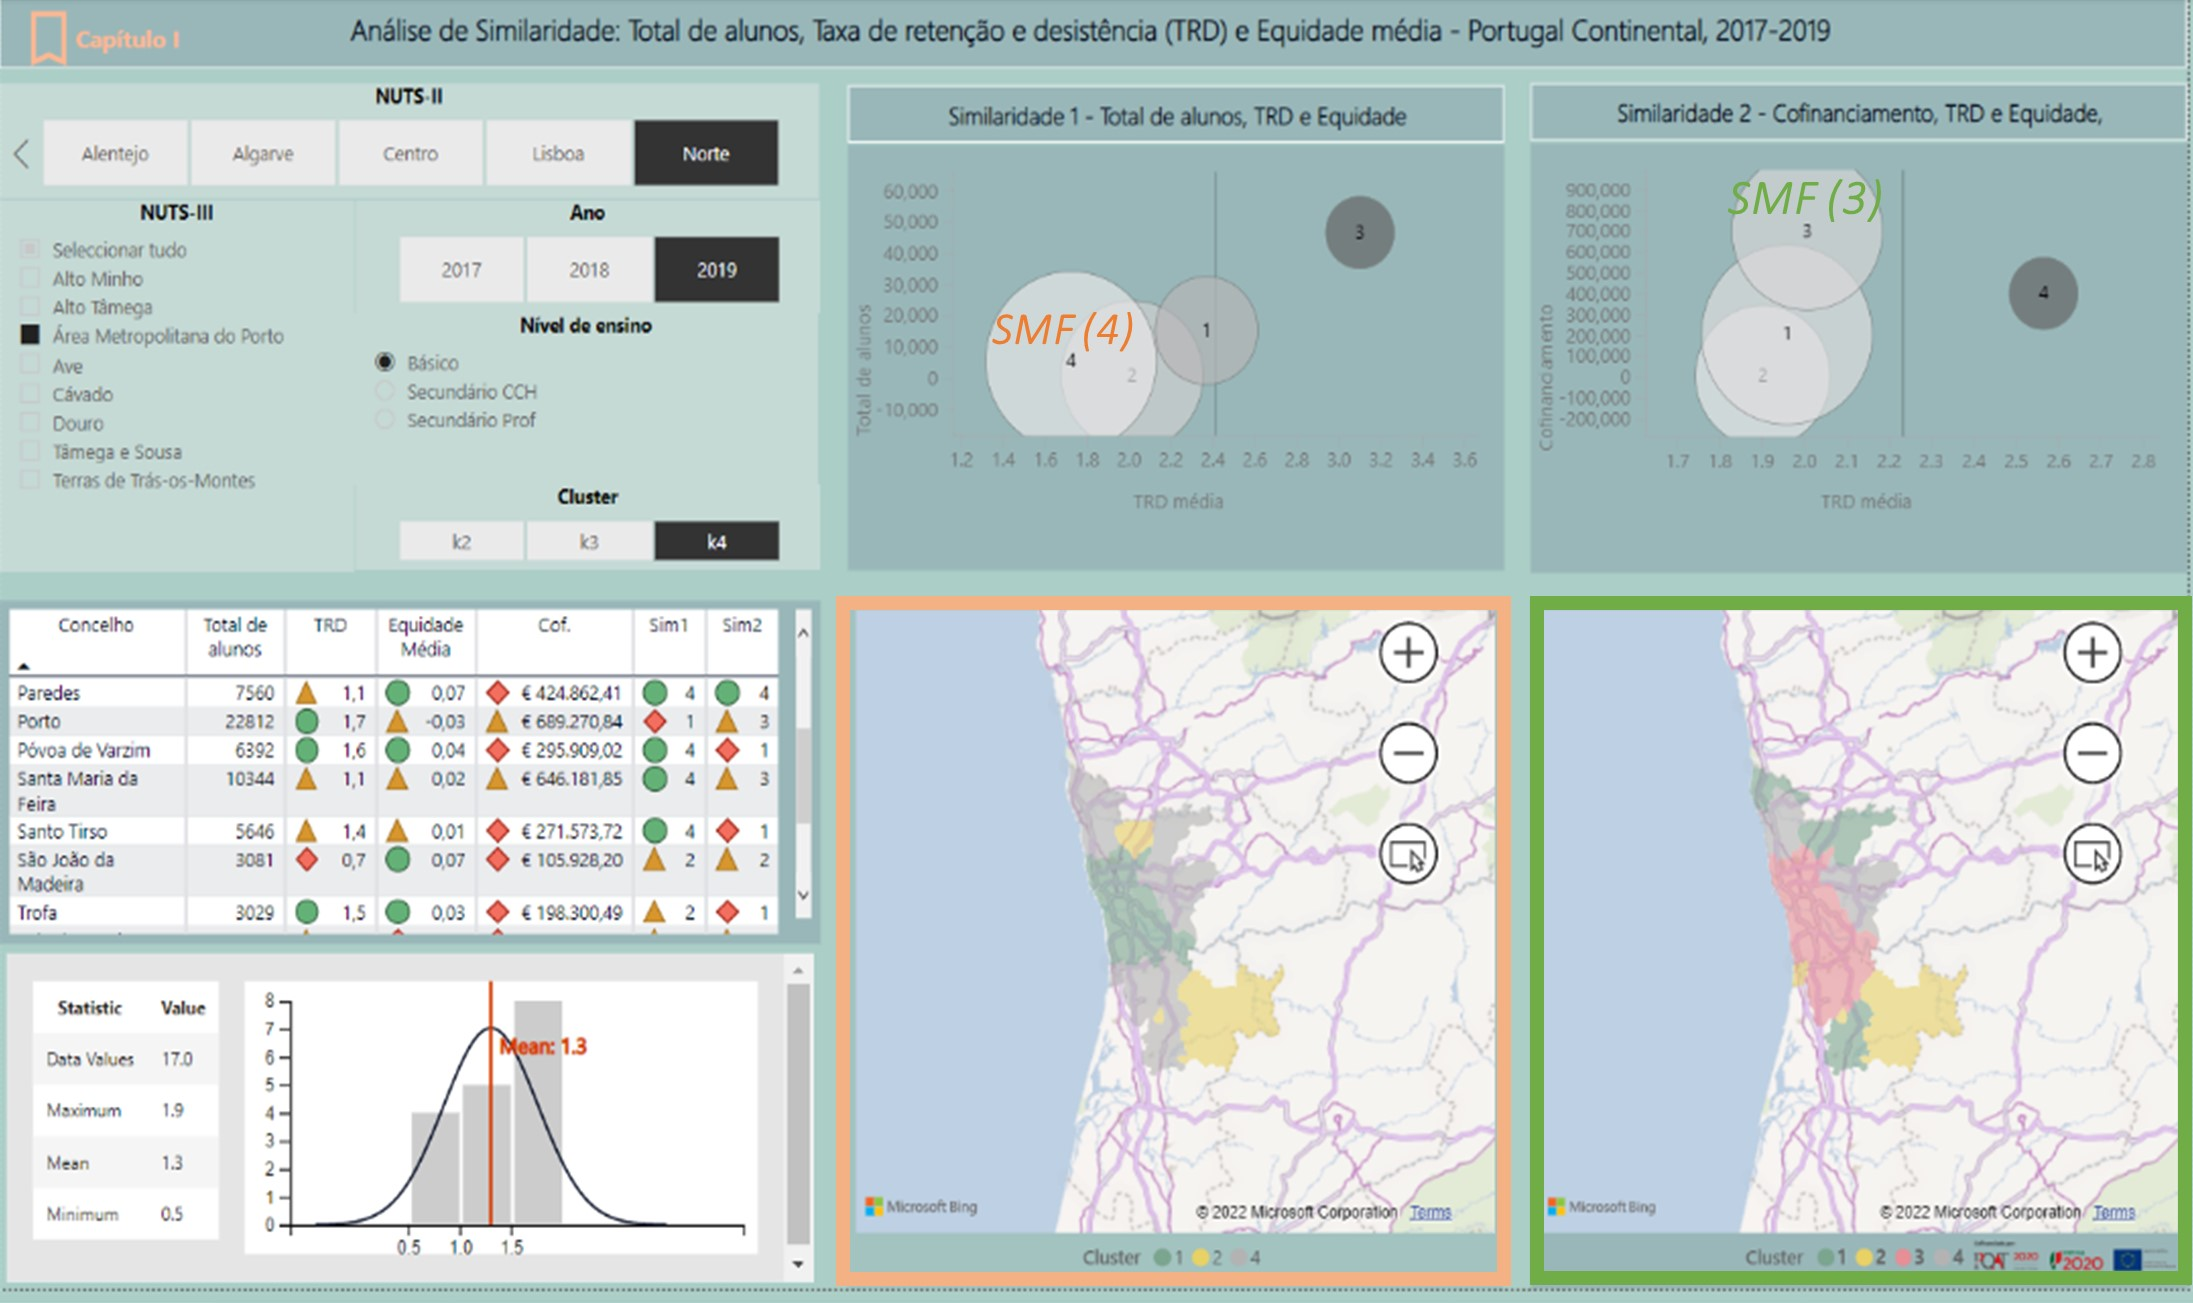
\includegraphics{C:/Users/julio/Documents/bookPoat/imagensRelatorio/figura38.jpg}
\caption{FIGURA 11: Capítulo I -- Caracterização do panorama educativo nacional: Painel da Análise de Similaridades, o exemplo do Ensino Básico Agregado, 2019/20 - FONTE: GETIN-UA}
\end{figure}

Um outro exemplo de aplicação deste tipo de análise, centra-se no comportamento das variáveis relativas ao ensino secundário em cursos CH, também para 2019/2020. No que ao município de SMF diz respeito, é possível observar, na figura seguinte, que este faz parte do \textbf{\emph{cluster 2}}, numa zona de transição da TRD (de baixa para alta TRD), alta equidade e baixo número de alunos face a valores médios nacionais \textbf{\emph{(similaridade 1)}}. Por outro lado, ao cruzar os indicadores de cofinanciamento, equidade e TRD, verifica-se que o município de SMF passa a integrar o \textbf{\emph{cluster 1}}, também numa área de transição da TRD \textbf{\emph{(similaridade 2)}}.

\begin{figure}
\centering
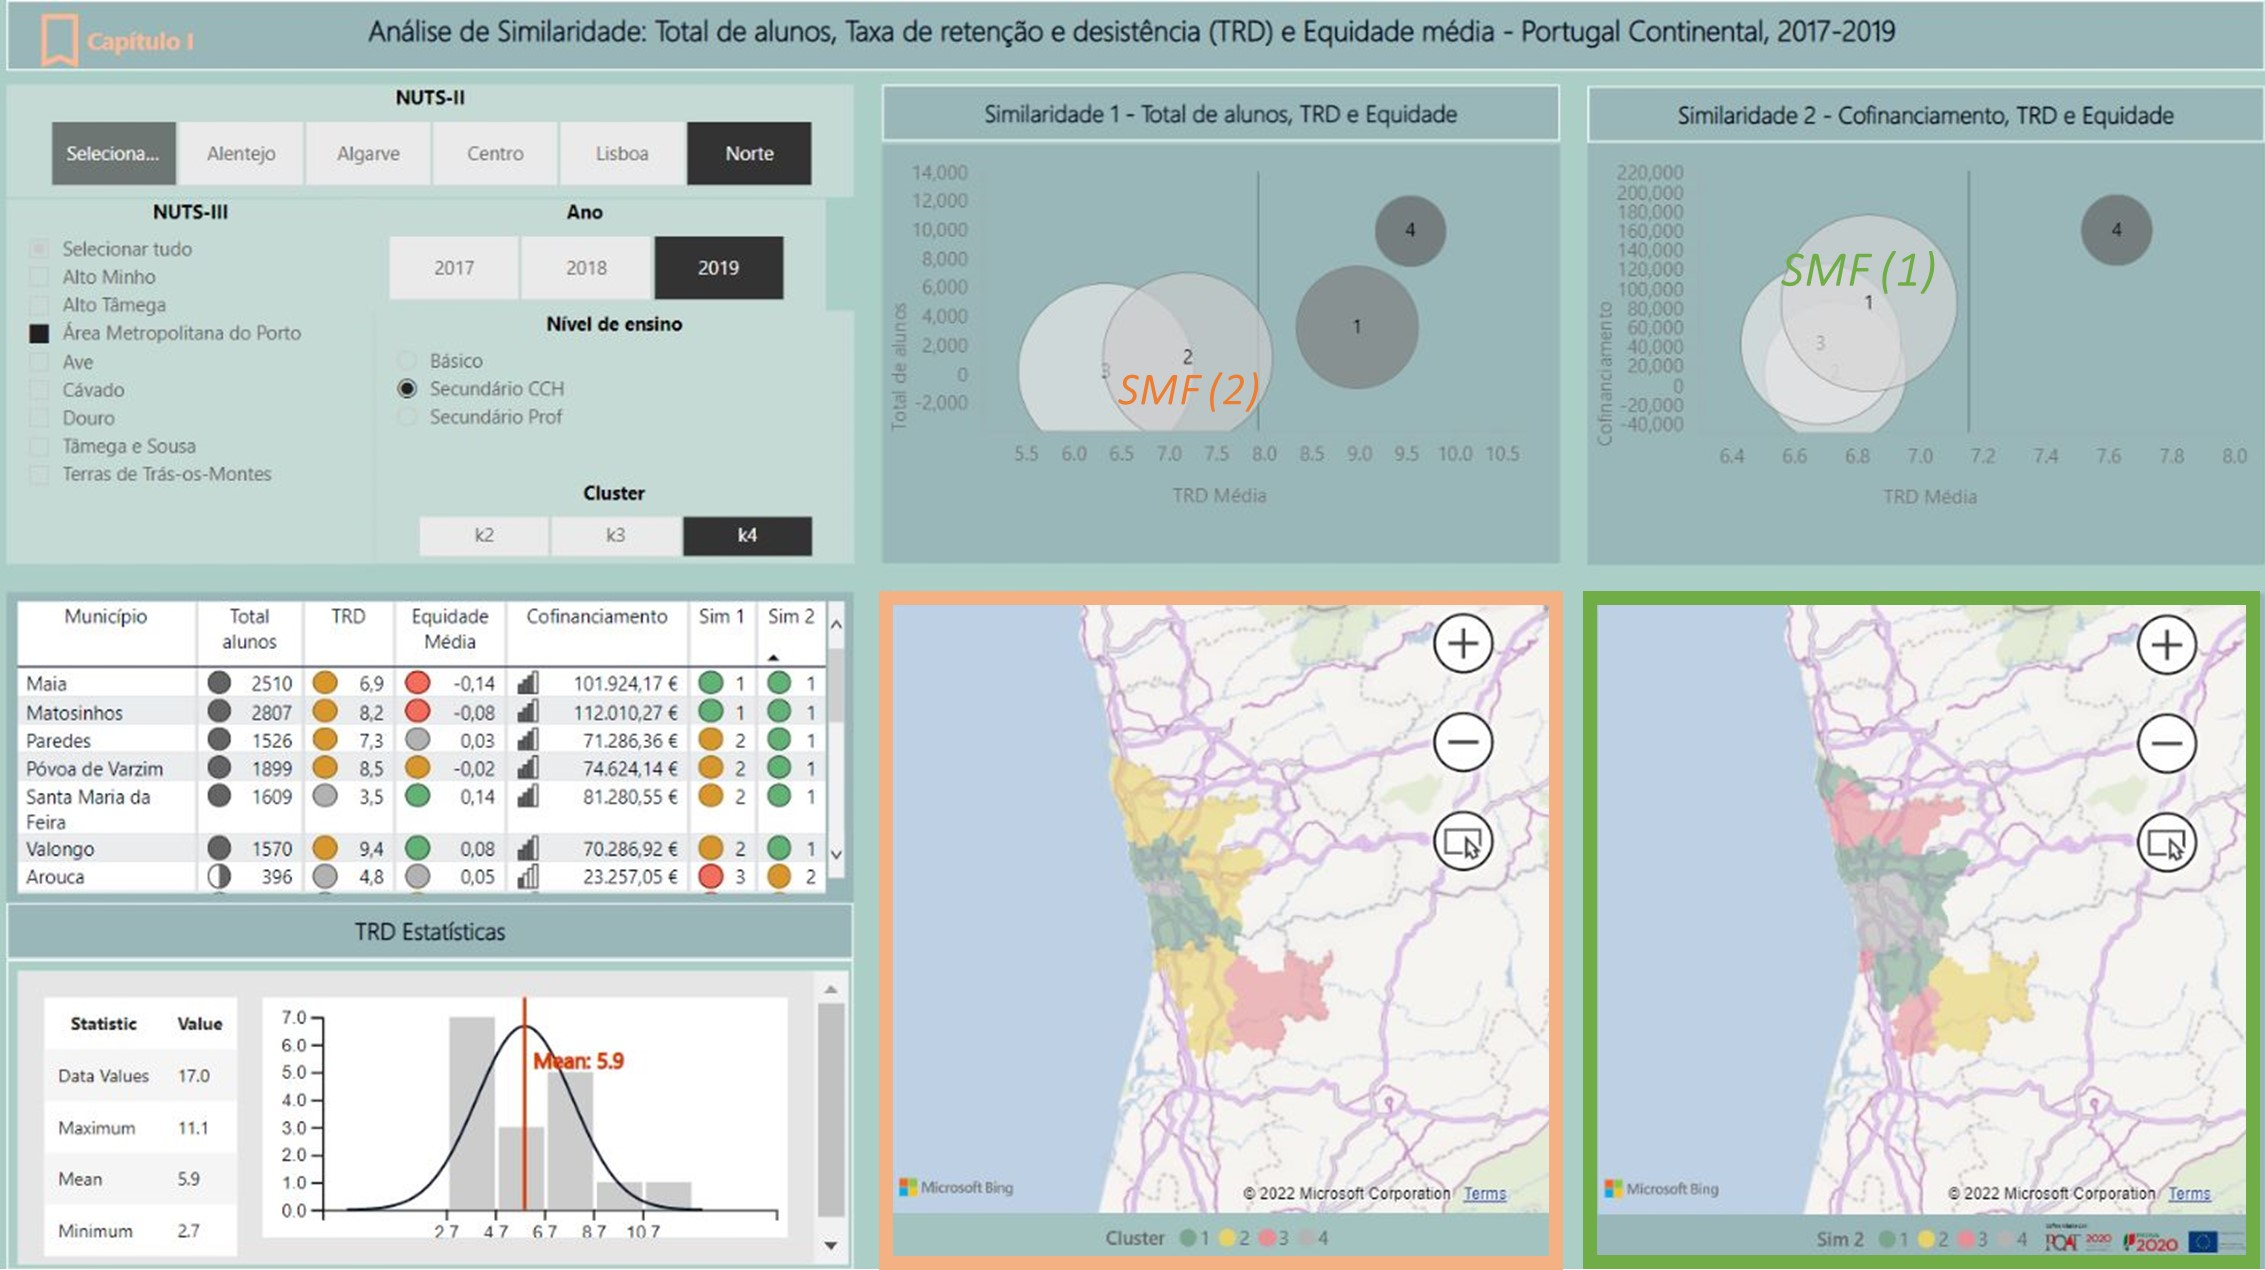
\includegraphics{C:/Users/julio/Documents/bookPoat/imagensRelatorio/figura39.jpg}
\caption{FIGURA 12: Capítulo I -- Caracterização do panorama educativo nacional: Painel da Análise de Similaridades, o exemplo do Ensino Secundário de CCH, 2019/20 - FONTE: GETIN-UA}
\end{figure}

Ao centrar a análise nos principais indicadores de desempenho escolar dos editais de candidatura dos PIICIE, TNN e TRD, é interessante observar e confrontar o respetivo comportamento ao longo do tempo. Uma primeira leitura é possível com recurso aos diagramas \emph{boxplots}, que permitem a comparação de ambas as taxas nos municípios da AMP. Os diagramas mostram ser particularmente úteis na fase exploratória do processo analítico-descritivo dos indicadores. Para além de apresentarem o menor e maior valores observados, permitem dividir cada grupo de dados (relativos a cada município) em quartis e fazer uma leitura comparada entre os grupos. Possibilitam ainda a identificação imediata de valores discrepantes do conjunto total de dados (chamados de \emph{outliers} e que aparecem sinalizados a vermelho).

Os \emph{outliers} que aparecem na parte inferior do diagrama, indicam escolas num dado município com TNN ou TRD significativamente menores face às demais. Identificadas estas escolas, poder-se-á, a partir de processos de \emph{benchmarking} em projetos futuros, tentar perceber as respetivas práticas pedagógicas e os motivos de resultados mais positivos quando comparadas com outras. Já os \emph{outliers} que aparecem na parte superior, traduzem escolas com TNN ou TRD mais elevadas considerando o conjunto de dados e que, eventualmente, requereram de intervenção para mitigar os efeitos de níveis negativos ou retenções tão elevados.

Na figura seguinte é possível analisar as TNN médias e as TRD médias, calculadas a partir de dados de escolas públicas (183) e AE (123) dos 17 municípios da AMP, numa série temporal que percorre os anos letivos de 2014/2015 a 2019/20 e de 2014/2015 a 2018/19. Enquanto as primeiras incidem sobre o 2º e 3º CEB, as segundas incluem dados desde o 1º CEB ao Ensino Secundário.

Da análise das TNN médias, destaca-se o município do Porto com a maior amplitude no 2º e 3º CEB e, em contraposição, o município da Trofa. Ao nível das TRD, as diferenças de amplitude são menos percetíveis nuns níveis de ensino face a outros, embora o Porto mantenha a maior amplitude de dados. Não obstante, nem sempre o território que reúne os dados mais discrepantes é aquele que apresenta as taxas médias mais elevadas, em ambas as taxas. A figura assinala com \textbf{X} os municípios com TNN e TRD médias mais elevadas.

\begin{figure}
\centering
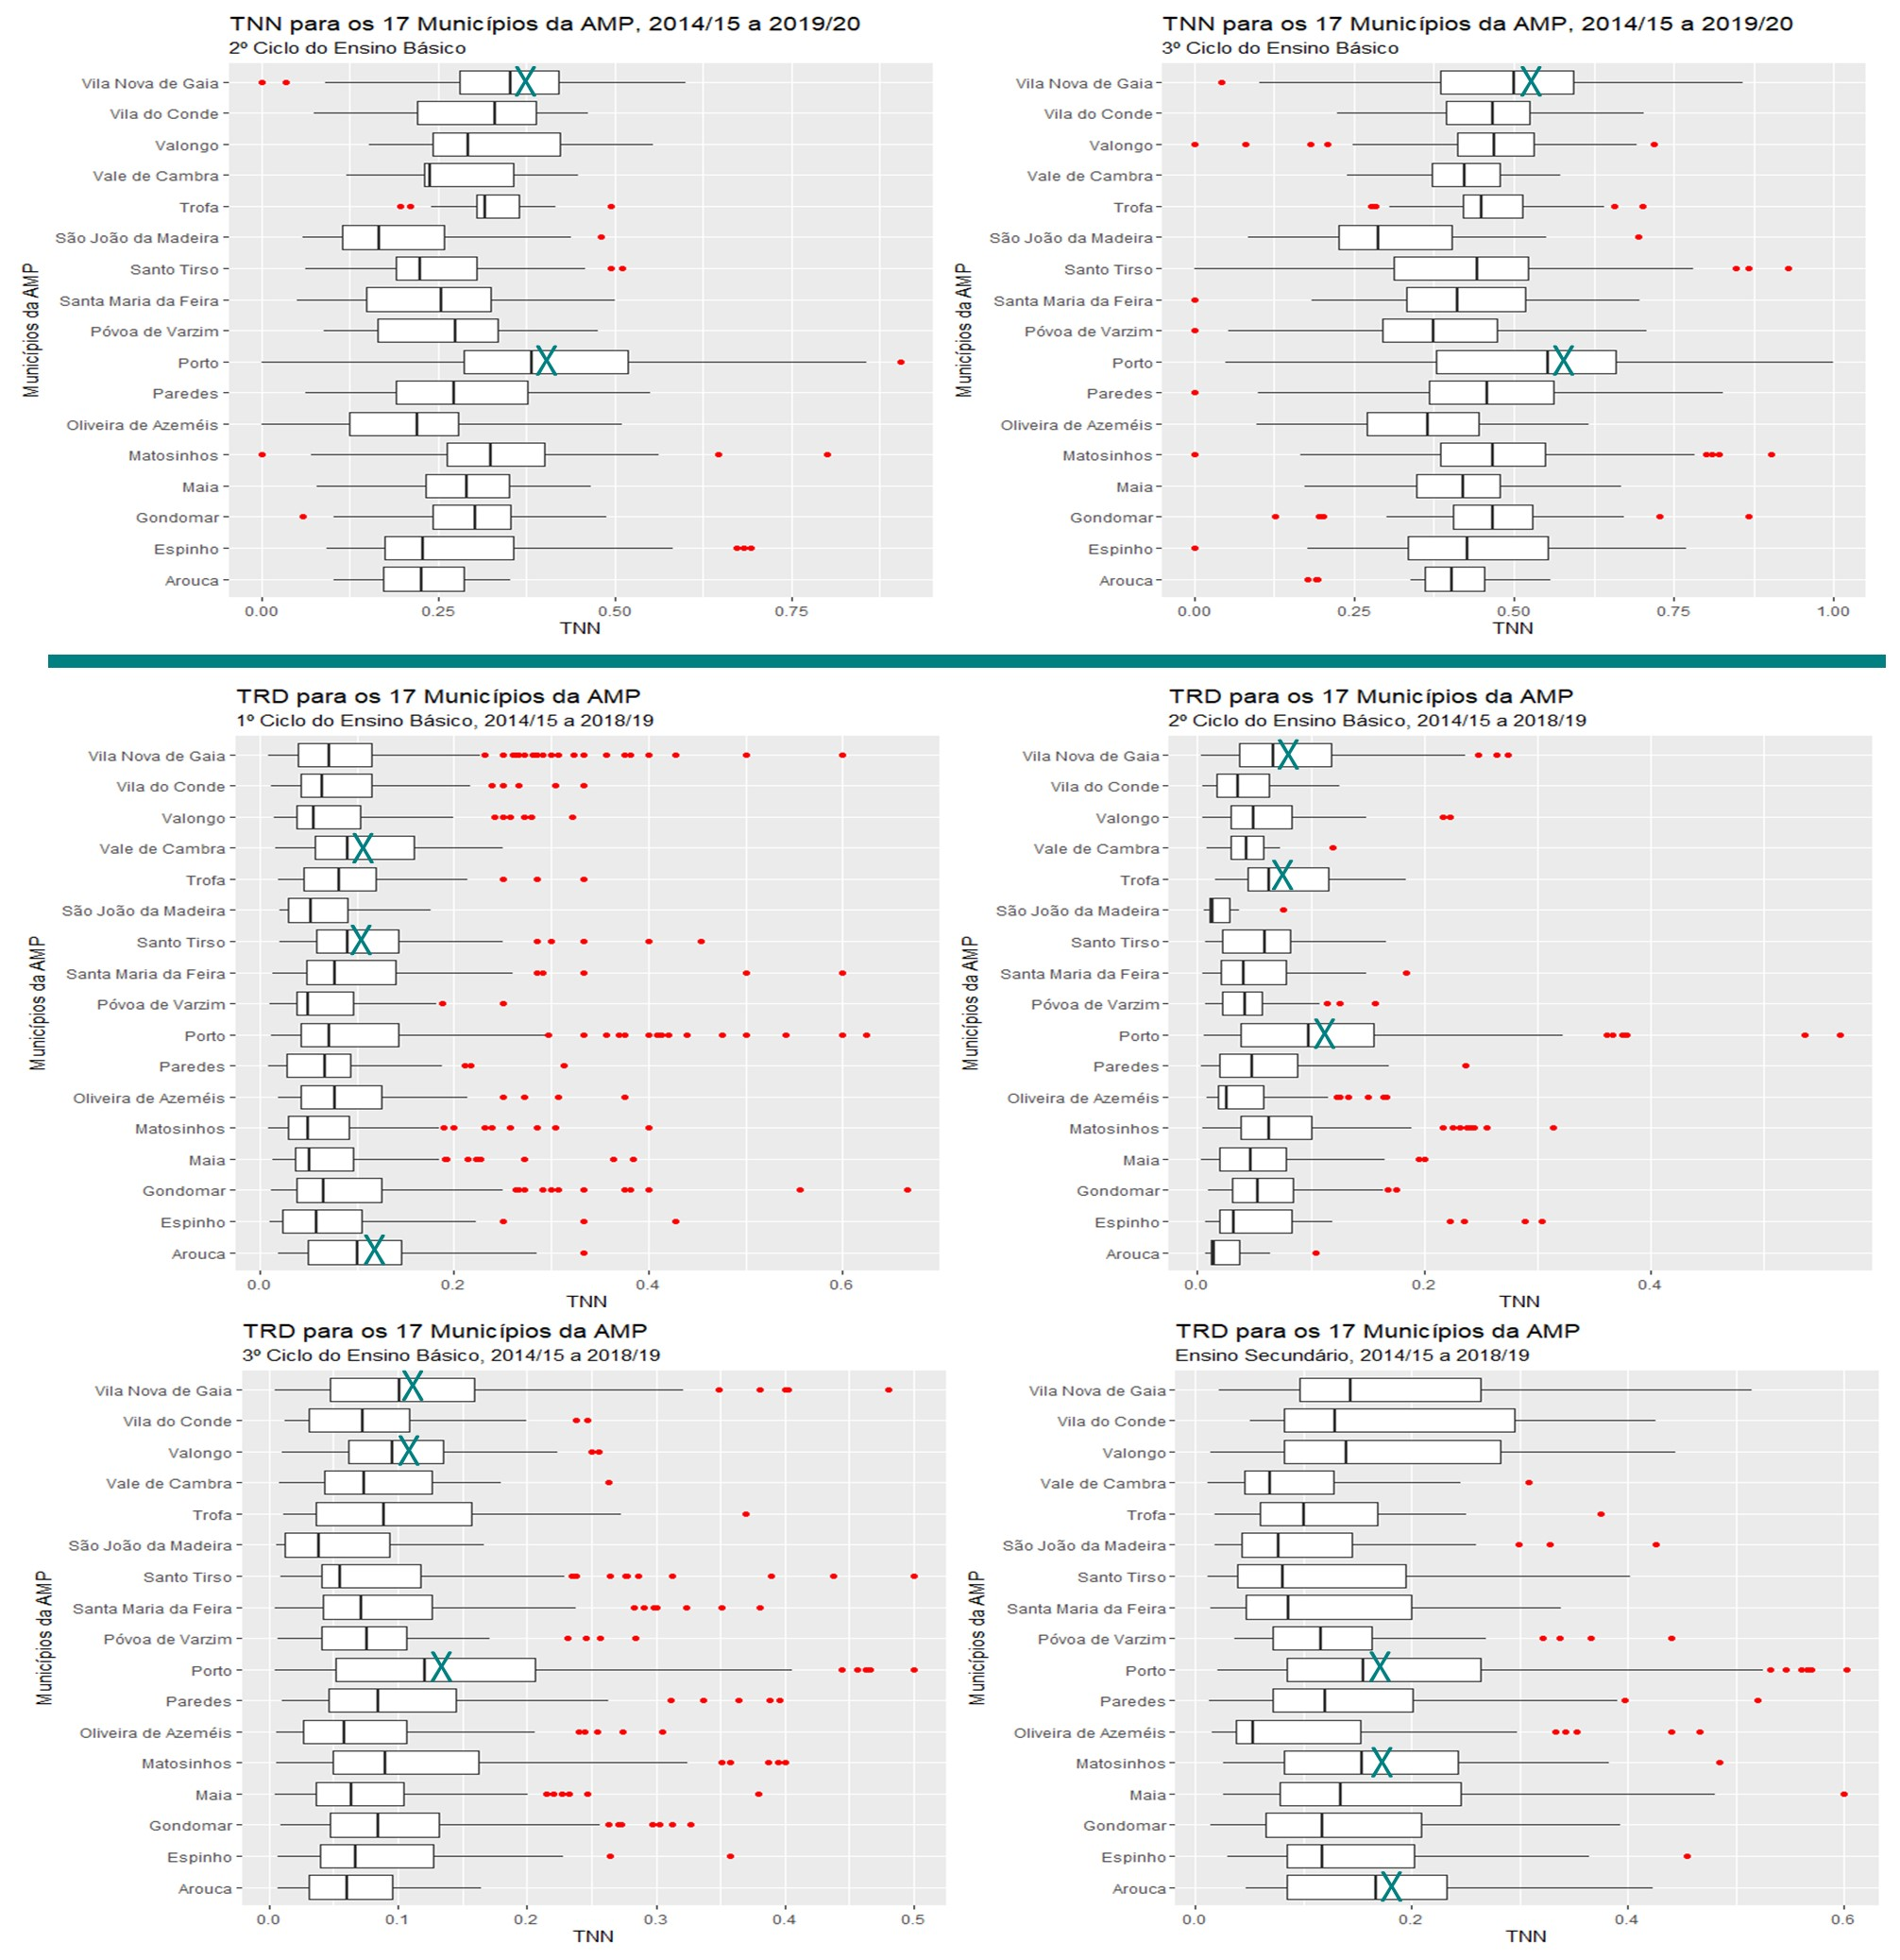
\includegraphics{C:/Users/julio/Documents/bookPoat/imagensRelatorio/figura40.jpg}
\caption{FIGURA 13: TNN médias e TRD médias para os 17 municípios da AMP - FONTE: Dados facultados pelo município de SMF, por sua vez fornecidos pela AMP (DGEEC)}
\end{figure}

Complementarmente, ao analisar os gráficos seguintes, que traduzem o contexto da AMP percebe-se que, tanto a TNN, como a TRD, diminuíram gradualmente ao longo da série temporal. Embora a tendência de diminuição seja notória nos diferentes níveis de ensino, partem de limiares distintos, verificando-se no caso das TNN que o 3º CEB ocupa um patamar claramente superior face ao 2CEB permanecendo bem acima no último ano letivo de análise e, no caso das TRD que os valores do 1º CEB estão naturalmente mais estabilizados ao passo que os do Secundário ainda refletem níveis de retenção expressivos.

\begin{figure}
\centering
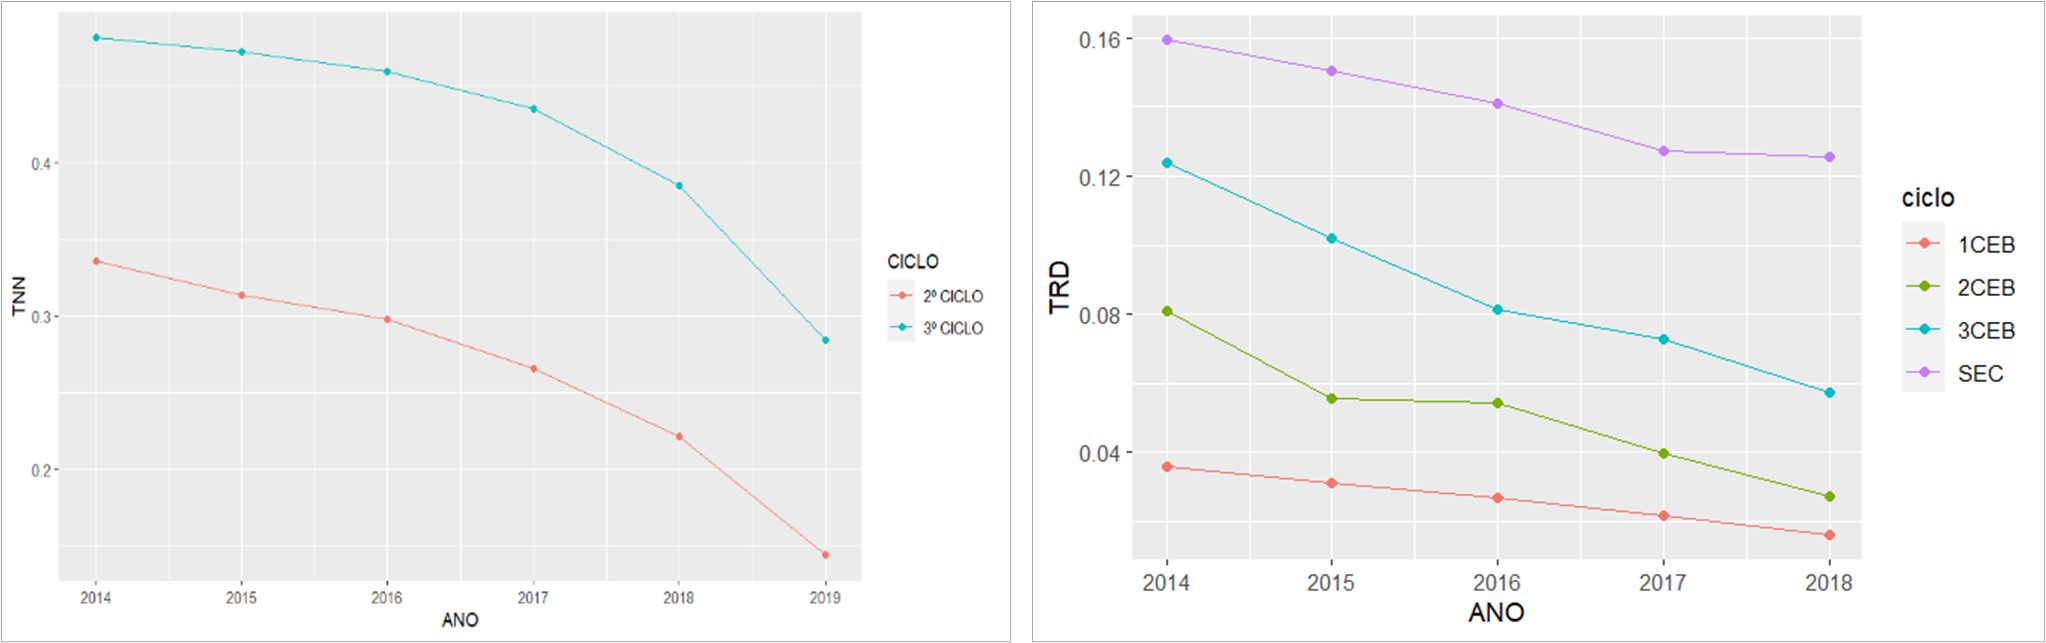
\includegraphics{C:/Users/julio/Documents/bookPoat/imagensRelatorio/figura41.jpg}
\caption{FIGURA 14: TNN 2014/15-2019/20 e TRD 2014/15-2018/19 para os 17 municípios da AMP - FONTE: Dados facultados pelo município de SMF, por sua vez fornecidos pela AMP (DGEEC)}
\end{figure}

Através do painel seguinte, é possível detalhar a análise das TNN e das TRD para os municípios da AMP, com desagregação até ao nível da escola (apenas são apresentados valores para escolas púbicas). Enquanto as TNN estão disponíveis para o 2º e 3º CEB, as TRD permitem uma digressão pelos quatro níveis de ensino. Os mapeamentos destacam a TNN e a TRD média no município de SMF (de 2014/15 a 2019/20 e de 2014/15 a 2018/19, respetivamente). Dados específicos do contexto de SMF mostram uma redução da TNN de 43,6\% em 2014/15 para 16,8\% em 2019/20 e da TRD de 5,9\% para 2,9\% em 2018/19.

\begin{figure}
\centering
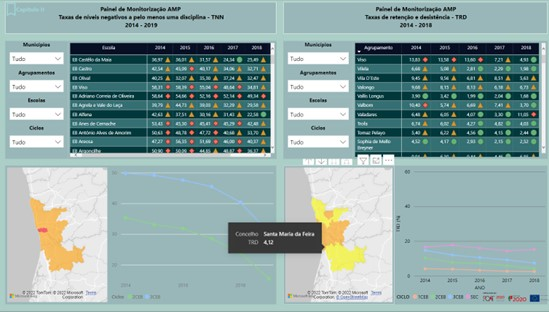
\includegraphics{C:/Users/julio/Documents/bookPoat/imagensRelatorio/figura42.jpg}
\caption{FIGURA 15: Capítulo II -- Caracterização do panorama educativo regional: TNN e TRD para os 17 municípios da AMP - FONTE: Dados facultados pelo município de SMF, por sua vez fornecidos pela AMP (DGEEC)}
\end{figure}

Para além da análise ao nível da AMP, a ferramenta permite também monitorizar as TNN e TRD registadas nas escolas públicas dos 9 AE de SMF, para os anos letivos das respetivas séries temporais.

\begin{figure}
\centering
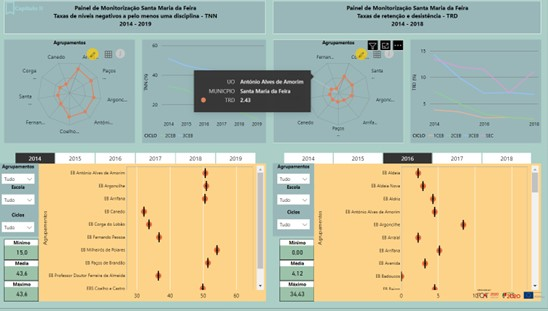
\includegraphics{C:/Users/julio/Documents/bookPoat/imagensRelatorio/figura43.jpg}
\caption{FIGURA 16: Capítulo II -- Caracterização do panorama educativo local: TNN e TRD para o município de SMF - FONTE: Dados facultados pelo município de SMF, por sua vez fornecidos pela AMP (DGEEC)}
\end{figure}

Apesar do comportamento semelhante, a análise exige olhares distintos para a TRD e para a TNN. Esta última tende a apresentar valores claramente superiores, uma vez que compreende os alunos que, com apenas uma negativa a uma disciplina, transitam de ano. A TRD inclui um grupo (infelizmente) mais seleto de alunos: aqueles que, somados os níveis negativos, não reuniam condições para a transição ou que desistem do ensino. Não obstante a tendência de diminuição, importa vigiar ambas as taxas, esperando-se que reflitam o impacto da conjuntura pandémica nas aprendizagens.

\hypertarget{possuxedveis-fatores-de-influuxeancia}{%
\section{\texorpdfstring{\textbf{Possíveis fatores de influência}}{Possíveis fatores de influência}}\label{possuxedveis-fatores-de-influuxeancia}}

Tendo presentes algumas das mensagens decorrentes dos pontos anteriores, optou-se por desenvolver uma análise complementar com o intuito de contribuir para uma reflexão mais alargada a respeito dos eventuais fatores de influência sobre os indicadores gerais de desempenho, em particular das TRD. Ainda que os resultados obtidos não permitam chegar a conclusões fechadas, contribuem para a teorização de aspetos que concorrem, de formas distintas, para os níveis de sucesso em diferentes níveis de ensino.

A análise aqui desenvolvida abrange os municípios da Região Norte e permite tecer algumas ilações acerca da influência destas unidades espaciais no comportamento das TRD das unidades vizinhas. A identificação de associações espaciais entre os municípios decorreu da análise i) de matrizes de pesos (k-vizinhos mais próximos, de distância a 100km e de Kernel), ii) do cálculo do Índice de Moran para cada matriz (para avaliar a existência de autocorrelação espacial) e iii) dos diagramas de dispersão de Moran e dos mapas LISA:

\begin{itemize}
\tightlist
\item
  O \textbf{Índice de Moran} é um indicador que permite aferir a semelhança geral entre regiões (neste caso, são considerados municípios). Quanto mais próximo de 1 for este índice, mais adequada será a utilização da matriz, devendo o seu nível de significância (p-sim) ser \textless{} 5\%;
\item
  Os \textbf{diagramas de dispersão de Moran} partem do cálculo do índice de Moran e, num referencial de 4 quadrantes, permitem visualizar a desfasagem espacial da variável das TRD (eixo dos y) e o desvio-padrão dessa mesma variável (eixo dos x). As autocorrelações (associações espaciais) positivas-fortes implicam semelhanças entre municípios vizinhos, as negativas-fortes traduzem dissemelhanças e as autocorrelações fracas refletem ausência de associação espacial:
\end{itemize}

\textbf{Quadrante Alto-Alto (Q1)}: municípios e vizinhos com valores elevados da TRD;\\
\textbf{Quadrante Baixo-Alto (Q2)}: municípios com valores baixos e vizinhos com valores elevados da TRD;\\
\textbf{Quadrante Baixo-Baixo (Q3)}: municípios e vizinhos com valores baixos da TRD;\\
\textbf{Quadrante Alto-Baixo (Q4)}: municípios com valores elevados e vizinhos com valores baixos da TRD;

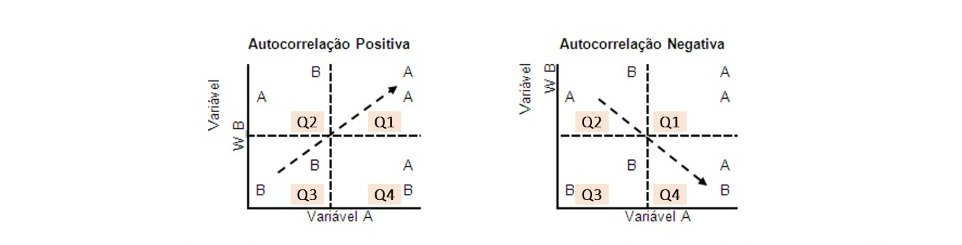
\includegraphics{C:/Users/julio/Documents/bookPoat/imagensRelatorio/figura9.jpg}

\begin{itemize}
\tightlist
\item
  Os \textbf{mapas LISA} traduzem espacialmente os resultados dos digramas de dispersão de Moran. As cores presentes, tanto no diagrama de dispersão de Moran como no mapa LISA, representam os quatro tipos de dependências relacionais entre vizinhos referidos anteriormente: \textbf{\emph{vermelho}} -- \emph{High-High} (municípios e vizinhos com valores elevados da TRD); \textbf{\emph{azul claro}} -- \emph{Low-High} (municípios com valores baixos e vizinhos com valores elevados da TRD); \textbf{\emph{azul escuro}} -- \emph{Low-Low} (municípios e vizinhos com valores baixos da TRD); \textbf{\emph{laranja}} -- \emph{High-Low} (municípios com valores elevados e vizinhos com valores baixos da TRD); \textbf{\emph{cinza}} -- municípios que não são significantes para a análise.
\end{itemize}

Na figura seguinte estão representados os diagramas de dispersão de Moran e os mapas LISA obtidos com a \textbf{matriz de Kernel para o 1ºCEB} e com a \textbf{matriz k-vizinhos mais próximos para os restantes níveis de ensino}. Estas foram as matrizes de pesos que mais se destacaram, surgindo com um Índice de Moran mais expressivo. Ao analisar o índice de Moran das matrizes selecionadas, percebe-se que, na generalidade, as autocorrelações ao nível das TRD no 2ºCEB, 3ºCEB e Secundário são positivas fracas, enquanto no 1ºCEB a autocorrelação é negativa fraca, com a maioria dos pontos correspondentes aos municípios do Índice de Moran afastados de 1.

Através dos mapas LISA, que mostram a espacialização da TRD por nível de ensino, importa salientar as seguintes mensagens:

\begin{itemize}
\tightlist
\item
  Ao nível do 1ºCEB, Tarouca surge com os valores mais elevados da variável dependente, ao contrário dos municípios vizinhos que apresentam valores baixos (\textbf{\emph{laranja}}). O município aparenta assim não ser influenciado pelos vizinhos;
\item
  Quanto ao 2ºCEB, os municípios da Maia, Porto e Gondomar são os territórios que aparecem com os valores mais elevados da TRD, verificando-se uma influência mútua entre estes e os municípios vizinhos que apresentam também valores elevados (\textbf{\emph{vermelho}}). Valpaços também se destaca, mas com um comportamento distinto ao nível da TRD, apresentando valores elevados enquanto os seus vizinhos apresentam valores baixos (\textbf{\emph{laranja}});
\item
  No 3ºCEB verifica-se influência entre os municípios de Vila do Conde, Matosinhos, Maia, Porto e Gondomar e os seus vizinhos, pois todos apresentam valores elevando da TRD (\textbf{\emph{vermelho}}). Já Bragança mostra um comportamento distinto dos vizinhos, o primeiro com valores baixos e os segundos com valores altos (\textbf{\emph{laranja}}). Ponte da Barca e Vila Verde, assim como os seus vizinhos, surgem com valores baixos da TRD (\textbf{\emph{azul escuro}});
\item
  No que respeita ao Secundário, Matosinhos, Porto e Gondomar apresentam valores elevados da TRD, tal como os municípios à sua volta, verificando-se uma clara influência (\textbf{\emph{vermelho}}). Já Celorico de Basto surge com valores elevados da TRD, enquanto os vizinhos apresentam baixos (\textbf{\emph{laranja}}). Miranda do Douro, pelo contrário, surge com valores baixos, ao passo que os vizinhos têm valores elevados (\textbf{\emph{azul claro}}). Nestes dois municípios deduz-se, assim, que não exista influência entre eles e os seus vizinhos.
\end{itemize}

Ainda que o comportamento da TRD no município de SMF nos diferentes níveis de ensino não seja significante para a análise (\textbf{\emph{cinza}}), como é o território de estudo do projeto, importa fazer referência ao seu posicionamento no conjunto. Pode depreender-se assim que, face aos municípios da Região Norte contemplados na análise sem exclusão, os valores da TRD se encontram dentro dos valores médios do grupo.

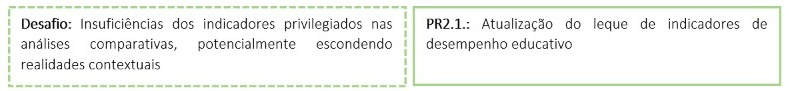
\includegraphics{C:/Users/julio/Documents/bookPoat/imagensRelatorio/figura44.jpg}

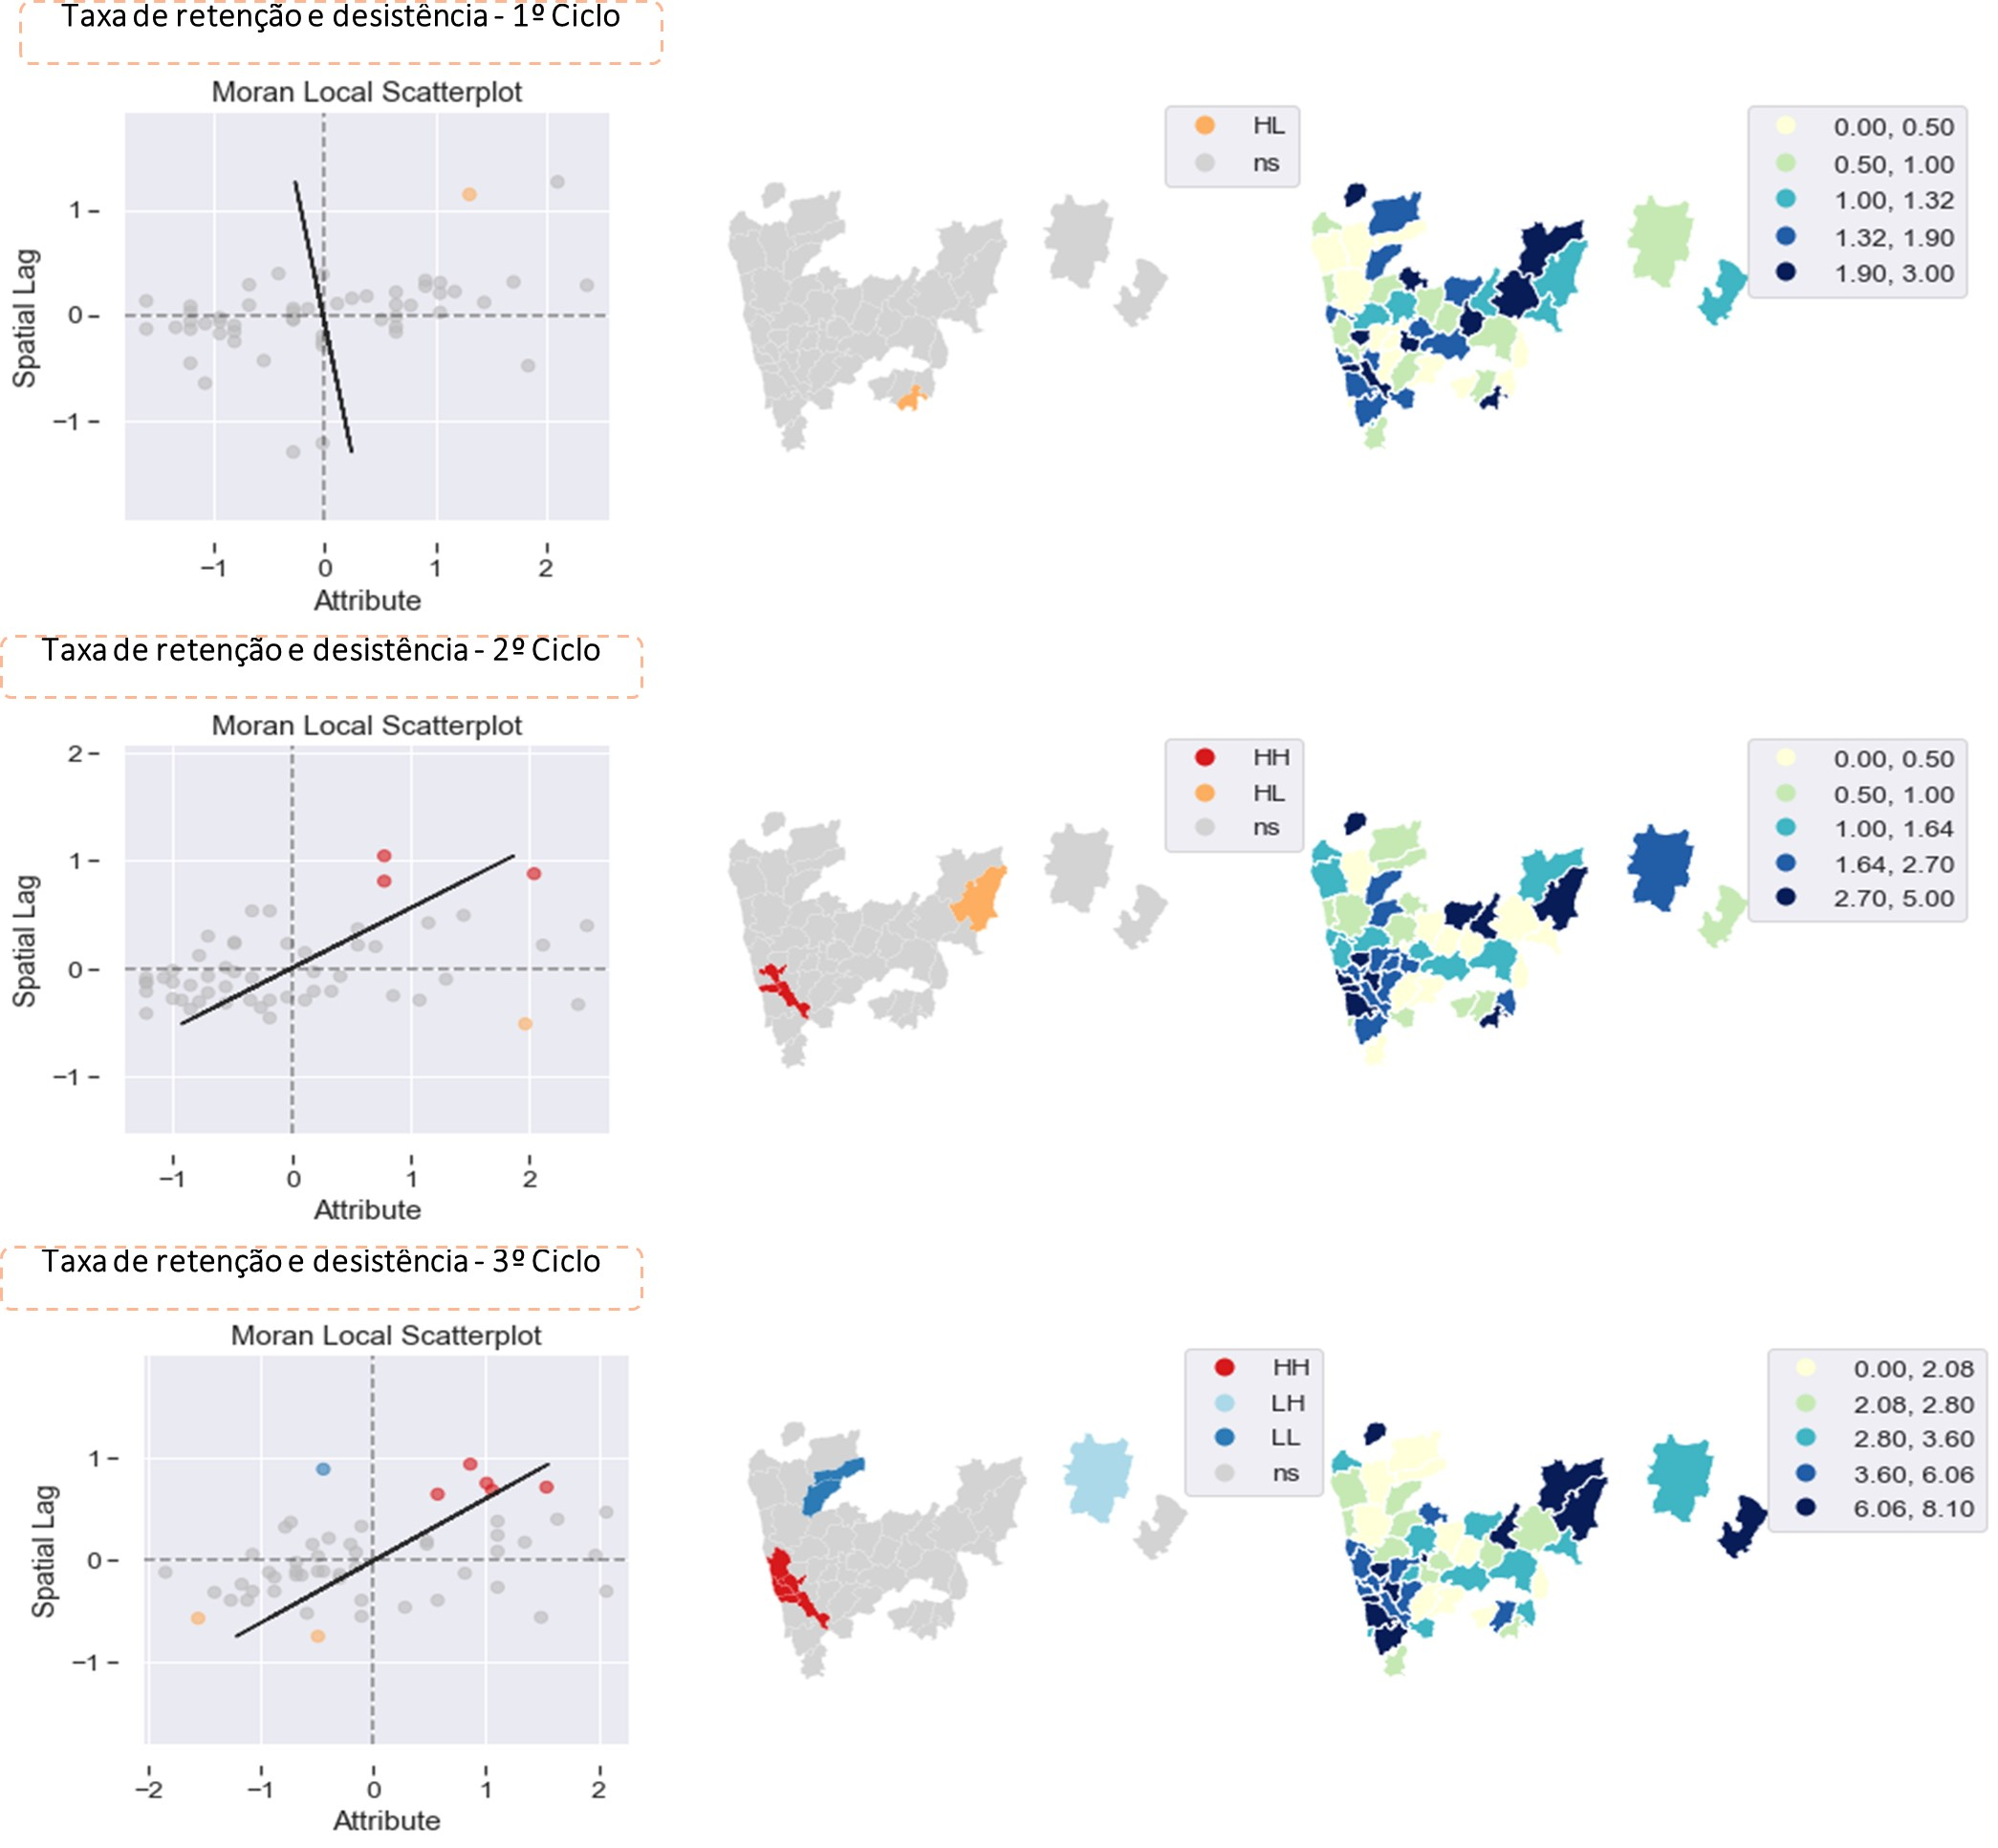
\includegraphics{C:/Users/julio/Documents/bookPoat/imagensRelatorio/figura45.jpg}

\begin{figure}
\centering
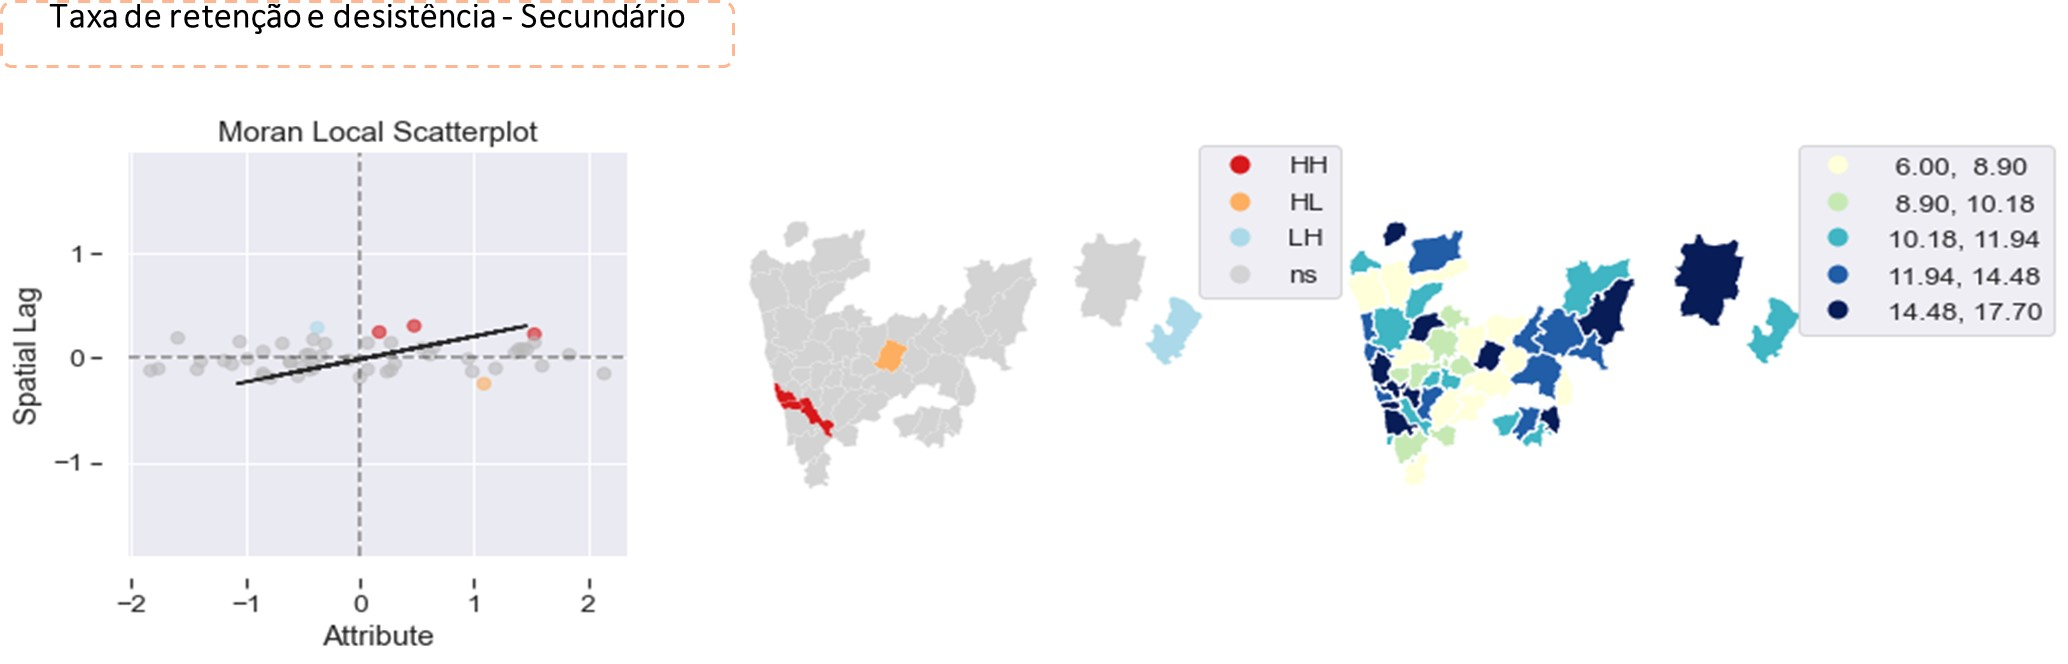
\includegraphics{C:/Users/julio/Documents/bookPoat/imagensRelatorio/figura46.jpg}
\caption{FIGURA 17: Diagramas de dispersão de Moran, mapas LISA e mapas de ajustamento da TRD por nível de ensino - FONTE: GETIN-UA -- Outputs gerados no software Python}
\end{figure}

Com o intuito de dar continuidade e robustecer a análise anterior, foram trabalhadas e integradas variáveis adicionais de caracterização educativa e socioeconómica, acreditando que a avaliação da existência de correlações entre elas pudesse contribuir para a identificação de possíveis fatores de influência da TRD nos diferentes níveis de ensino. A matriz de autocorrelação que se segue, entre TDR e variáveis assumidas como independentes/explicativas, pretende assim contribuir para este exercício.

\begin{figure}
\centering
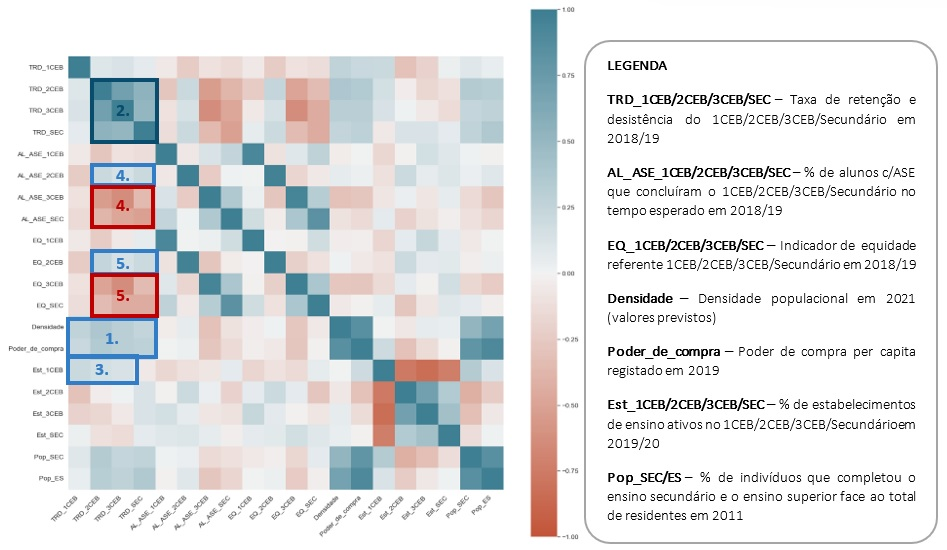
\includegraphics{C:/Users/julio/Documents/bookPoat/imagensRelatorio/figura47.jpg}
\caption{FIGURA 18: Matriz de correlação entre as TRD e as variáveis explicativas - FONTE: GETIN-UA -- Outputs gerados no software Python / Origem dos dados: DGEEC, Infoescolas, Pordata}
\end{figure}

Por observação da matriz, é possível destacar algumas mensagens acerca da influência das variáveis independentes sobre as TRD, de entre as quais se destacam as seguintes:

\textbf{1.} Em todos os níveis de ensino, as TRD (TRD\_1CEB, TRD\_2CEB, TRD\_3CEB, TRD\_SEC) apresentam uma \textbf{correlação positiva} com a densidade populacional e o poder de compra per capita (\textbf{\emph{azul petróleo médio}}); acredita-se que esta relação poderá ser explicada pelo facto de territórios mais densamente povoados tenderem a incorporar o efeito gerado por assimetrias territoriais;

\textbf{2.} A \textbf{correlação positiva forte} estabelecida entre as TRD de níveis intermédios e avançados (TRD\_2CEB, TRD\_3CEB, TRD\_SEC) (\textbf{\emph{azul petróleo escuro}}); as interdependências entre as TRD a partir do 2ºCEB sugerem alguma influência que poderá decorrer de fragilidades não ultrapassadas pelos alunos neste nível e comprometer a sequencialidade do percurso educativo e formativo no tempo esperado;

\textbf{3.} Entre as TRD dos ciclos do ensino básico (1º, 2º e 3º) e a \% de estabelecimentos de ensino com 1ºCEB verifica-se, também, uma \textbf{correlação positiva} (\textbf{\emph{azul petróleo médio}}); o que poderá indiciar que um maior número de escolas de pequena dimensão no primeiro nível de ensino nem sempre poderá desencadear melhores níveis de desempenho escolar na prossecução e conclusão do ensino básico;

\textbf{4.} As TRD do 2ºCEB, 3ºCEB e Secundário estabelecem uma \textbf{correlação positiva} com a \% de alunos com ASE que concluíram o 2ºCEB em 2 anos (\textbf{\emph{azul petróleo médio}}), enquanto a sua combinação com a \% de alunos com ASE que concluíram o 3ºCEB e o Secundário no tempo esperado traduzem uma \textbf{correlação negativa forte} (\textbf{\emph{vermelho escuro}}); estes resultados exploratórios sugerem que o 2ºCEB poderá constituir um patamar de clivagem entre progressão vs retenção na escada de qualificações;

\textbf{5.} Complementarmente, observa-se que a TRD do 2ºCEB, 3ºCEB e Secundário estabelece uma \textbf{correlação positiva} com a equidade no 2ºCEB (\textbf{\emph{azul petróleo médio}}), ao passo que no 3ºCEB e Secundário essa \textbf{correlação é negativa forte} (\textbf{\emph{vermelho escuro}}); por outras palavras, se maiores níveis de equidade acabam por ser determinantes no sucesso escolar dos alunos no 3ºCEB e Secundário, ao nível do 2ºCEB isso não se verifica, reforçando a mensagem do ponto anterior.

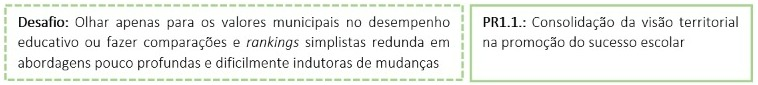
\includegraphics{C:/Users/julio/Documents/bookPoat/imagensRelatorio/figura48.jpg}

\hypertarget{o-piicie-de-santa-maria-da-feira}{%
\chapter{\texorpdfstring{\textbf{O PIICIE de Santa Maria da Feira}}{O PIICIE de Santa Maria da Feira}}\label{o-piicie-de-santa-maria-da-feira}}

\hypertarget{breve-caracterizauxe7uxe3o-territorial-e-educativa-do-municuxedpio}{%
\section{\texorpdfstring{\textbf{Breve caracterização territorial e educativa do município}}{Breve caracterização territorial e educativa do município}}\label{breve-caracterizauxe7uxe3o-territorial-e-educativa-do-municuxedpio}}

O Município de Santa Maria da Feira é um território dinâmico e palco de diversidades que se traduzem na natureza plural dos seus territórios educativos. À semelhança de outros concelhos do país e das regiões onde se insere (AMP e Região Norte), enfrenta desafios i) que emergem de singularidades e assimetrias internas, ii) que decorrem do panorama de evolução que se perspetiva para o médio e longo prazo e iii) que se enquadram em reptos mais abrangentes ligados a orientações nacionais e transnacionais. Assim, a compreensão das opções estratégicas na promoção do sucesso escolar em Santa Maria da Feira não poderá ser dissociada das características socioeducativas e dos referenciais de partida recentes na quantificação e interpretação dos níveis de desempenho que apresenta.

Com uma elevada dinâmica empresarial, associativa e cultural, bem como um forte histórico industrial, mais presente em algumas freguesias, o concelho de Santa Maria da Feira assinalou na última década uma evolução considerável dos níveis de qualificação da sua população residente (INE, 2021). As taxas de retenção, um dos principais indicadores abordados no estudo, pelo contrário, mostram uma diminuição e valores de referência abaixo dos da região e do país (DGEEC, 2022b). Ainda que estas sejam tendências transversais a vários territórios do país, importa sublinhar que a Educação tem sido assumida como área prioritária de intervenção no município de estudo, à qual tem sido dada crescente visibilidade. A candidatura realizada para elaboração do PIICIE municipal é disso exemplo, assim como o Projeto Educativo Municipal 2014'20 e mais recentemente o Plano Estratégico Educativo Municipal 2022-30, instrumentos que têm contribuído para a definição e afirmação das políticas educativas locais em articulação com outras áreas como a cultura, o desporto ou a economia.

A necessidade de acompanhar as respetivas dinâmicas e políticas educativas municipais tem conduzido, igualmente, a um investimento em medidas de monitorização, visando um olhar integrado sobre a implementação, o acompanhamento e a avaliação de projetos e iniciativas em matéria de educação, promovidas pelo município, mas também por outros agentes territoriais. Muitas destas iniciativas terão como objetivo específico promover o sucesso escolar, enquanto noutras o propósito será mais alargado e direcionado a outros domínios da área educativa, mas nem por isso menos relevantes na elevação e consolidação dos padrões de qualidade do sistema de ensino à escala local.

A riqueza e multiplicidades que povoam o concelho justificam a diversidade encontrada ao nível da rede educativa, da qual fazem parte, atualmente, 124 instituições desde a educação pré-escolar ao ensino superior (Marques et al., n.d.). \textbf{A oferta pública conta com 85 estabelecimentos escolares distribuídos por 9 Agrupamentos de Escolas (AE)}. A escola de proximidade, isto é, aquela que corresponde aos primeiros níveis de educação e ensino (educação pré-escolar e 1º ciclo do ensino básico), é garantida nas 21 freguesias. E, naturalmente, que territórios centrais do concelho que têm registado, inclusive, um crescimento populacional coincidem com as áreas de influência dos agrupamentos de escolas com mais alunos inscritos: AE de Santa Maria da Feira e AE de Fernando Pessoa. Simultaneamente, várias instituições integram e contribuem para a qualificação da rede de ofertas educativas e formativas do concelho, como as instituições da rede solidária com educação pré-escolar, os centros de formação profissional públicos, as instituições privadas independentes do estado, as instituições de ensino artístico especializado, as instituições que salvaguardam a valência de creche e a instituição com oferta de ensino superior.

\begin{figure}
\centering
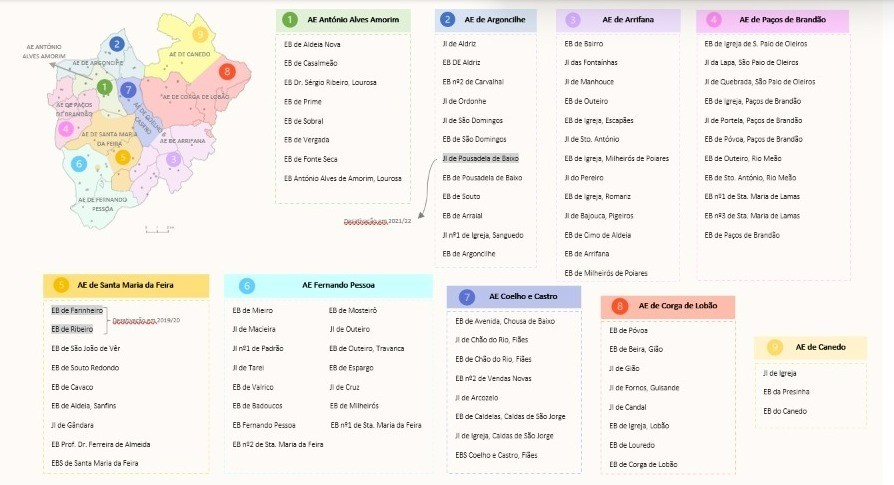
\includegraphics{C:/Users/julio/Documents/bookPoat/imagensRelatorio/figura14.jpg}
\caption{FIGURA 19: Esquematização da Rede Educativa Agrupada do Município de Santa Maria da Feira - FONTE: GETIN-UA -- PEEM 2022-2030}
\end{figure}

\hypertarget{apresentauxe7uxe3o-e-descriuxe7uxe3o-do-piicie}{%
\section{\texorpdfstring{\textbf{Apresentação e descrição do PIICIE}}{Apresentação e descrição do PIICIE}}\label{apresentauxe7uxe3o-e-descriuxe7uxe3o-do-piicie}}

O PIICIE de Santa Maria da Feira integra seis ações que iniciaram a 12 de outubro de 2018 e terminaram a 31 de dezembro 2021. A \textbf{Ação 1 - Equipa Multidisciplinar} centra-se, essencialmente, na prevenção e na intervenção em casos de alunos que demonstram dificuldades em aprender e com risco de abandono escolar. A \textbf{Ação 2 - Vive as Férias} promove a aquisição de diversas competências ao nível individual e social, através de atividades lúdicas e criativas. A \textbf{Ação 3 - Observatório de Monitorização e Apoio ao Sucesso Escolar} foi criada com o objetivo de todos os munícipes conseguirem acompanhar de forma rigorosa as políticas educativas implementadas em Santa Maria da Feira. Já a \textbf{Ação 4 - Educação 5.0} foca-se no desenvolvimento de valores importantes para que as crianças, professores e pais tenham capacidade de exercer um papel ativo na comunidade. Para além disso, esta ação pressupõe a criação de um ambiente tecnológico de modo a favorecer a partilha de informação e o trabalho colaborativo. A \textbf{Ação 5 - Hora de Programar} tem como princípios a inovação e a criatividade e é através destes princípios que pretende consolidar aprendizagens na área das ciências, matemática e leitura. Na \textbf{Ação 6 - Hora de Experimentar} são abordados fenómenos da natureza com o auxílio da ciência. Assim, os alunos têm oportunidade de fazer experiências e, simultaneamente, aprender sobre ações do quotidiano.

Analisando a natureza e o espírito das ações de uma perspetiva global, destacam-se princípios como a cooperação e a colaboração, remetendo para o principal objetivo da criação do PIICIE, isto é, \textbf{o foco no trabalho em rede para o desenvolvimento do município e para a capacitação da comunidade}.

No total, participaram cerca de 18.657 alunos nas ações do PIICIE\footnote{Excetuam-se os participantes que poderiam estar associados à Ação 3, cuja contabilização não foi reunida.}. A ação Educação 5.0 destaca-se com o maior número de participantes pelo facto de integrar tanto os participantes das Olimpíadas da Cidadania e do Património, nos anos de 2019/20 e 2020/21, como também todos os alunos envolvidos na atribuição de tablets às escolas no início de 2018.

Três das principais mais-valias do PIICIE de Santa Maria da Feira passam pela diversidade dos domínios das ações, pela promoção da articulação interinstitucional e pela iniciativa municipal em dar continuidade temporal e estender o PIICIE a outros públicos para lá do cofinanciamento, assumindo a despesa. Aparenta, ainda, haver uma razoável visibilidade deste plano e entendimento em torno do seu valor.

\textbf{Diversidade temática}

O desenho e implementação deste PIICIE assente em várias áreas temáticas traduz diferentes mensagens relevantes e que podem inspirar outros programas:

\begin{enumerate}
\def\labelenumi{\arabic{enumi}.}
\item
  Entende-se que o combate ao insucesso escolar se faz por meio de diferentes tipologias de ação e que apenas uma abordagem simultaneamente multifacetada e integrada poderá ser bem-sucedida;
\item
  Ainda que alinhada com o discurso educativo da UE voltado para a sociedade baseada no conhecimento e para a competitividade (Nóvoa, 2013), a estratégia feirense aparenta ultrapassar esta visão estritamente económica e limitada da Educação, promovendo a inclusão, coesão e trabalho junto da/para a comunidade;
\item
  A aposta estratégica em áreas STEM como centrais no sucesso escolar e pessoal dos indivíduos (ilustrada através das ações Hora de Experimentar e Hora de Programar).
  Ainda que haja uma ligação entre o PIICIE e a estratégia local para a Educação, ficam de fora da espinha dorsal do projeto algumas áreas estratégicas de Santa Maria da Feira, como as Artes ou o Desporto, ainda que se entenda que estas são centrais para o sucesso escolar (Marques et al., n.d.). No entanto, esta opção limita as redundâncias e permite à política cofinanciada cumprir o seu valor acrescentado (Mairate, 2007).
\end{enumerate}

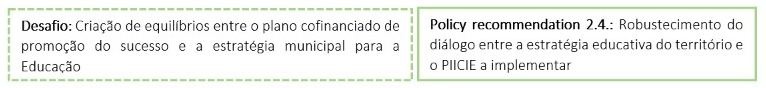
\includegraphics{C:/Users/julio/Documents/bookPoat/imagensRelatorio/figura49.jpg}

\textbf{Articulação interinstitucional}

As ações refletem o espírito de articulação com diversos agentes, essenciais para a concretização das metas. Foram várias as entidades parceiras que apoiaram a realização das ações, destacando-se a ação 1 - Equipa Multidisciplinar que requereu um maior número de parcerias (18), uma vez que as sessões do projeto Desafia-TE foram realizadas com diversos agentes de diferentes áreas. Estes agentes atuam no território e com a comunidade, assim conhecendo as suas especificidades e podendo encetar uma ação direcionada.

\textbf{Continuidade extra-cofinanciamento}

Apesar de ter sido definido que todas as ações do PIICIE de Santa Maria da Feira terminariam a 31 de dezembro de 2021, algumas ações, pelo seu impacto e sucesso, tiveram continuidade no ano letivo seguinte (Ação 1 -- Equipa Multidisciplinar). Outras foram alargadas a escolas e/ou públicos não contemplados inicialmente, pelo que os custos financeiros da extensão destas atividades e projetos ficaram a cargo do Município. É o caso da Ação 6 -- Hora de Experimentar, alargada a outras escolas, ou a Ação 4 -- Educação 5.0, uma vez que o uso da plataforma digital foi alargado à Educação Pré-Escolar.

\textbf{Visibilidade e apreciação espontânea}

O relatório final do plano `EDUFEIR@ - Inovamos para o Sucesso', elaborado pela entidade beneficiária, entende que as evidências recolhidas, medidas através de inquéritos e de contributos qualitativos, permitem inferir um grau de satisfação superior a 90\% (a meta estabelecida em sede de candidatura). Paralelamente a este projeto financiado pelo POAT, parte da equipa está envolvida na construção do Plano Estratégico Educativo Municipal (PEEM) 2022-2030 de Santa Maria da Feira, no âmbito do qual difundiu um inquérito de avaliação do anterior Projeto Educativo Municipal (PEM) 2014'20. Com elevada adesão (898 respostas válidas), vários respondentes mencionaram, em questões de resposta aberta, o PIICIE, nomeadamente quando inquiridos sobre ``programas, instrumentos e orientações internacionais, nacionais e regionais que tenham contribuído para melhorar a educação no concelho de SMF''\footnote{Fonte: Questões II.1. e II.1.1. do Inquérito de Satisfação face ao PEM 2014'20.}. Destacam-se, nessas respostas, a plataforma Edufeira, seguida dos programas Vives e do Desafia-TE.

\hypertarget{auxe7uxe3o-1---equipa-multidisciplinar}{%
\subsection{\texorpdfstring{\textbf{Ação 1 - Equipa Multidisciplinar}}{Ação 1 - Equipa Multidisciplinar}}\label{auxe7uxe3o-1---equipa-multidisciplinar}}

Foram desenvolvidos dois projetos: Sessões de acompanhamento de alunos com medidas adicionais\footnote{O artigo 10º do Decreto-Lei 54/2018 define que as medidas adicionais ``visam colmatar dificuldades acentuadas e persistentes ao nível da comunicação, interação, cognição ou aprendizagem que exigem recursos especializados de apoio à aprendizagem e à inclusão'' (Presidência do Conselho de Ministros, 2018).} na EB Corga de Lobão e o Desafia-TE. O primeiro projeto compreendia sessões quinzenais de orientação e suporte dos alunos, envolvendo atividades realizadas tanto em contexto escolar como no exterior. Realizaram-se atividades na área do desporto, da saúde e da cultura.

O Projeto Desafia-TE conta com a colaboração dos agrupamentos de escolas do município e diversos parceiros locais para a realização de sessões em locais diferentes todas as semanas. O processo de seleção para o Desafia-TE inclui sessões de divulgação em cada sede de agrupamento, seguidas de inscrições e entrevistas individuais, sendo que todos os anos o grupo de alunos selecionados é alterado. Assim, este projeto pretende proporcionar experiências diferentes de cariz desportivo, cultural, cívico, entre outras, aos selecionados, de forma a transmitir uma visão comunitária e inclusiva.

\hypertarget{auxe7uxe3o-2-vive-as-fuxe9rias}{%
\subsection{\texorpdfstring{\textbf{Ação 2 -- Vive as Férias}}{Ação 2 -- Vive as Férias}}\label{auxe7uxe3o-2-vive-as-fuxe9rias}}

Os programas VIVES ocorrem nos três períodos de férias letivas (na Páscoa, Verão e Natal) e têm duração de uma semana para cada grupo de alunos inscritos. Durante esta semana são realizadas atividades, principalmente nas áreas desportiva e cultural, que promovem a criatividade e a inovação, bem como o foco no desenvolvimento de competências individuais e de convivência. As planificações das atividades têm em consideração as idades e as particularidades de cada grupo de alunos.

\hypertarget{auxe7uxe3o-3-observatuxf3rio-de-monitorizauxe7uxe3o-e-apoio-ao-sucesso-escolar}{%
\subsection{\texorpdfstring{\textbf{Ação 3 -- Observatório de monitorização e apoio ao sucesso escolar}}{Ação 3 -- Observatório de monitorização e apoio ao sucesso escolar}}\label{auxe7uxe3o-3-observatuxf3rio-de-monitorizauxe7uxe3o-e-apoio-ao-sucesso-escolar}}

O Observatório de Monitorização e Apoio ao Sucesso Escolar tinha como pretensões o acompanhamento das políticas educativas, a monitorização dos indicadores de níveis de sucesso e a sua correlação com dados socioeconómicos. A construção e atualização permanente desta ferramenta serviriam tanto os decisores políticos no planeamento municipal da educação, como a comunidade educativa e qualquer cidadão que aceda aos painéis públicos da plataforma. Uma adicional mais-valia do Observatório residiria na integração do sistema de informação de apoio ao sistema educativo, assim cruzando indicadores. Este projeto permitiria o reforço da tomada de decisão com base em evidências, assim como uma maior transparência e \emph{accountability}.

\hypertarget{auxe7uxe3o-4-educauxe7uxe3o-5.0}{%
\subsection{\texorpdfstring{\textbf{Ação 4 -- Educação 5.0}}{Ação 4 -- Educação 5.0}}\label{auxe7uxe3o-4-educauxe7uxe3o-5.0}}

Esta ação desenvolveu três projetos: a plataforma digital Edufeira, aquisição de tablets e ações de capacitação. A plataforma Edufeira destina-se aos alunos do 1º CEB, professores e encarregados de educação e surge como um elemento facilitador de aprendizagem e de partilha de conhecimento, de forma a promover o trabalho colaborativo. Os conteúdos partilhados abrangem temáticas acerca do património de Santa Maria da Feira, cidadania, apoio ao estudo e atividades/desafios para fazer em família. Nos anos letivos 2019/20 e 2020/21, realizou-se o concurso ``Olimpíadas do Património'' para alunos de 3º e 4º ano, onde cada aluno participou individualmente, sendo apurada a melhor turma. Da 1ª fase resultaram nove turmas vencedoras, uma por cada agrupamento de escolas. Na fase final, as turmas apuradas competiram entre si e escolheu-se a vencedora consoante a pontuação adquirida.

Associado a este projeto, o município adquiriu cerca de 1200 tablets para equipar as 55 escolas de 1º ciclo, contribuindo para a utilização da plataforma em contexto de sala de aula. As ações de capacitação têm como objetivo divulgar e informar os participantes acerca de práticas educativas promotoras de mudança. Alguns exemplos de ações de capacitação desenvolvidas no âmbito da ação Educação 5.0 são a Oficina de Formação Professores e as Jornadas da Educação.

\hypertarget{auxe7uxe3o-5-hora-de-programar}{%
\subsection{\texorpdfstring{\textbf{Ação 5 -- Hora de Programar}}{Ação 5 -- Hora de Programar}}\label{auxe7uxe3o-5-hora-de-programar}}

No âmbito da ação Hora de Programar foram realizadas sessões quinzenais junto dos alunos de 1º, 2º e 3º CEB com o objetivo de desenvolver competências na área da tecnologia e da programação com o apoio dos professores. A realização de trabalhos escolares nestas sessões promoveu o trabalho em grupo e incentivou o relacionamento entre os alunos. Para além das sessões em contexto escolar, alguns dos alunos participaram no evento Robô Oeste e no Concurso nacional de programação ``A Criar com \emph{Scratch}!''.

\hypertarget{auxe7uxe3o-6-hora-de-experimentar}{%
\subsection{\texorpdfstring{\textbf{Ação 6 -- Hora de Experimentar }}{Ação 6 -- Hora de Experimentar }}\label{auxe7uxe3o-6-hora-de-experimentar}}

A ação Hora de Experimentar foi realizada em quatro agrupamentos do município: Argoncilhe, Arrifana, Santa Maria da Feira e Coelho e Castro. Estes agrupamentos apostaram nas ciências experimentais e desenvolveram sessões quinzenais, onde os alunos têm espaço para fazer experiências científicas e explorar novos desafios. Esta ação promove o raciocínio e a cooperação entre os alunos, fazendo com que estes adquiram novas competências na área da ciência.

\hypertarget{indicadores-de-resultado-e-realizauxe7uxe3o-da-operauxe7uxe3o-cofinanciada}{%
\section{\texorpdfstring{\textbf{Indicadores de resultado e realização da operação cofinanciada}}{Indicadores de resultado e realização da operação cofinanciada}}\label{indicadores-de-resultado-e-realizauxe7uxe3o-da-operauxe7uxe3o-cofinanciada}}

Partilha-se do entendimento avançado pelo relatório de Avaliação do Contributo do PT2020 para a Promoção do Sucesso Educativo, Redução do Abandono Escolar Precoce e Empregabilidade dos jovens, uma vez que não é possível

\begin{quote}
\emph{``estabelecer uma relação direta entre os projetos PIICIE e a evolução das taxas de retenção/desistência (pois o território é beneficiário de um conjunto muito mais lato de medidas que podem fazer a diferença)''} (IESE et al., 2021, p.~81)
\end{quote}

Este \emph{caveat} não deve, no entanto, impedir uma análise dos indicadores, designadamente das taxas de retenção e desistência (TRD) e das taxas de níveis negativos (TNN) no território em estudo, indicadores contratualizados pela entidade beneficiária. Por outro lado, a leitura dos resultados deve, ainda, estar consciente da conjuntura crítica pandémica, contemporânea de parte do período de análise. Recorre-se a exemplos retirados dos painéis de informação construídos no âmbito do presente projeto.

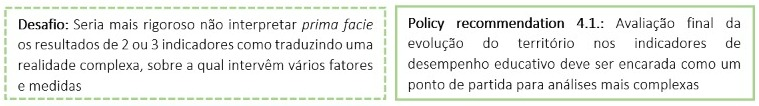
\includegraphics{C:/Users/julio/Documents/bookPoat/imagensRelatorio/figura50.jpg}

\begin{longtable}[]{@{}lll@{}}
\toprule()
Alunos envolvidos nas atividades, por nível de ensino & & \\
\midrule()
\endhead
Meta contratualizada & Resultados & \\
4.200 & 18.657\footnote{Este valor pode diferir do relatório final de Candidatura PIICIE do Município de Santa Maria da Feira, devido a uma atualização e correção posteriores dos dados.} & \\
\bottomrule()
\end{longtable}

A meta foi amplamente ultrapassada, destacando-se, em número total de participantes, o AE Fernando Pessoa.

Medidas de cada operação implementadas

\begin{longtable}[]{@{}lll@{}}
\toprule()
Medidas de cada operação implementadas & & \\
\midrule()
\endhead
Meta contratualizada & Resultados & \\
\textgreater80\% & Entende-se que a meta foi cumprida & \\
\bottomrule()
\end{longtable}

O relatório final do PIICIE Edufeira refere que ``Todas as ações foram executadas, até em período de suspensão das atividades letivas e não letivas presencias, decorrentes da pandemia COVID-19, com exceção de algumas das atividades da ação 2 -- Vive as Férias'' (Câmara Municipal de Santa Maria da Feira, 2022: 35).

\begin{figure}
\centering
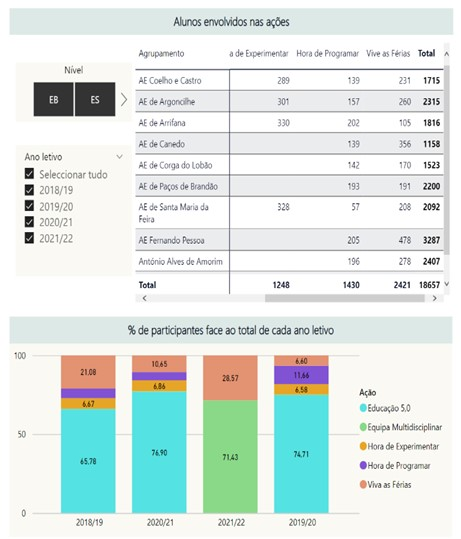
\includegraphics{C:/Users/julio/Documents/bookPoat/imagensRelatorio/figura51.jpg}
\caption{FIGURA 20: Capítulo IV -- Participantes nas 6 ações do PIICIE de SMF - FONTE: Dados facultados pelo município de SMF}
\end{figure}

\begin{longtable}[]{@{}lll@{}}
\toprule()
Municípios envolvidos na operação & & \\
\midrule()
\endhead
Meta contratualizada & Resultados & \\
1 & 1 & \\
\bottomrule()
\end{longtable}

\begin{longtable}[]{@{}lll@{}}
\toprule()
Agrupamentos abrangidos & & \\
\midrule()
\endhead
Meta contratualizada & Resultados & \\
100\% & 100\% (9/9 AE abrangidos) & \\
\bottomrule()
\end{longtable}

\begin{longtable}[]{@{}lll@{}}
\toprule()
Redução da taxa de alunos com níveis negativos & & \\
\midrule()
\endhead
Meta contratualizada & Resultados & \\
\textgreater10\% & 2.º CEB: -55\% / 3.º CEB: -46\% & \\
\bottomrule()
\end{longtable}

Verifica-se uma expressiva redução da taxa de alunos com níveis negativos (TNN) a pelo menos uma disciplina, ainda que se mantenham assimetrias entre os Agrupamentos.

\begin{figure}
\centering
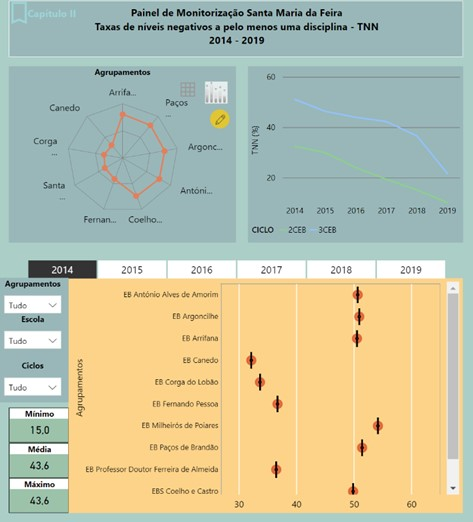
\includegraphics{C:/Users/julio/Documents/bookPoat/imagensRelatorio/figura52.jpg}
\caption{FIGURA 21: Capítulo II -- TNN nos AE do município de SMF - FONTE: Município de SMF/AMP(DGEEC)}
\end{figure}

\begin{longtable}[]{@{}
  >{\raggedright\arraybackslash}p{(\columnwidth - 4\tabcolsep) * \real{0.3333}}
  >{\raggedright\arraybackslash}p{(\columnwidth - 4\tabcolsep) * \real{0.3333}}
  >{\raggedright\arraybackslash}p{(\columnwidth - 4\tabcolsep) * \real{0.3333}}@{}}
\toprule()
\begin{minipage}[b]{\linewidth}\raggedright
Redução da taxa de retenção e desistência
\end{minipage} & \begin{minipage}[b]{\linewidth}\raggedright
\end{minipage} & \begin{minipage}[b]{\linewidth}\raggedright
\end{minipage} \\
\midrule()
\endhead
Meta contratualizada & Resultados & \\
\textgreater25\% & 1.º CEB: -44\% 2.º CEB: -64\% 3.º CEB: -74\% Ens. Sec.: -42\% & \\
\bottomrule()
\end{longtable}

Da mesma forma, a taxa de retenção e desistência (TRD) assistiu, durante o mesmo período, a uma clara redução. Não obstante, os anos que se seguem à implementação do PIICIE podem revelar-se críticos, uma vez que é expectável uma tradução mais real do impacto do contexto pandémico e do consequente encerramento das escolas.

\begin{figure}
\centering
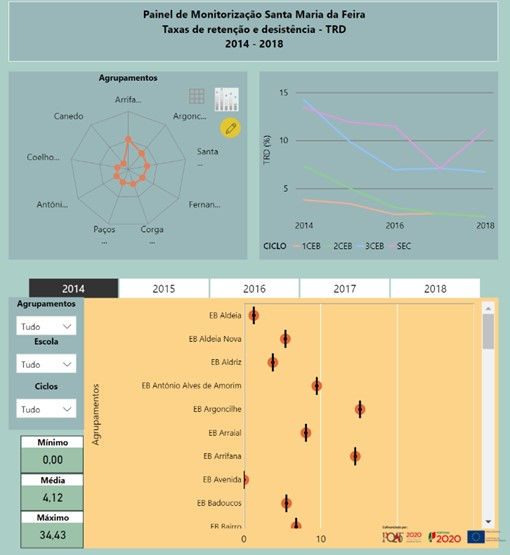
\includegraphics{C:/Users/julio/Documents/bookPoat/imagensRelatorio/figura53.jpg}
\caption{FIGURA 22: Capítulo II -- TRD nos AE do município de SMF - FONTE: Município de SMF/AMP (DGEEC)}
\end{figure}

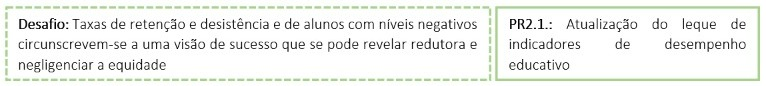
\includegraphics{C:/Users/julio/Documents/bookPoat/imagensRelatorio/figura54.jpg}

\begin{longtable}[]{@{}lll@{}}
\toprule()
Grau de satisfação & & \\
\midrule()
\endhead
Meta contratualizada & Resultados & \\
90\% & Entende-se que a meta foi cumprida & \\
\bottomrule()
\end{longtable}

Recorrendo a questionários difundidos nos anos letivos 2019/20 e 2020/21, bem como a pareceres solicitados aos AE aquando do término do projeto, a entidade beneficiária concluiu que a meta contratualizada de 90\% foi atingida (Câmara Municipal de Santa Maria da Feira, 2022). De uma forma geral, os agrupamentos de escolas salientam a importância que o PIICIE teve nos processos de aprendizagem e colaboração para o combate ao insucesso escolar. Destaca-se a necessidade de dar continuidade a vários projetos desenvolvidos e o alargamento destes para todos os alunos, uma vez que produziram experiências inovadoras e úteis no percurso escolar destes, considerando-os um benefício para o município de Santa Maria da Feira. Para além dos agrupamentos, a Fapfeira evidenciou que, apesar dos constrangimentos causados pela pandemia COVID-19, a implementação dos projetos ocorreu de forma positiva, cumprindo as metas propostas. Foi aconselhado, por parte da associação, investir numa maior divulgação das atividades desenvolvidas de forma a informar o maior número de pessoas e aumentar a adesão aos projetos.

Para a análise integrada do panorama educativo local em SMF, houve um esforço na construção de painéis de informação que permitissem, ao nível dos AE, uma leitura cruzada entre indicadores gerais de desempenho (TRD e TNN) e indicadores de caracterização socioeducativa (equidade e \% de alunos com ASE que concluíram os estudos no tempo esperado). Na figura seguinte, é assim possível analisar o desempenho escolar nos 9 AE, recorrendo a variáveis mais estritas e mais latas de aferição dos respetivos níveis de (in)sucesso.

\begin{figure}
\centering
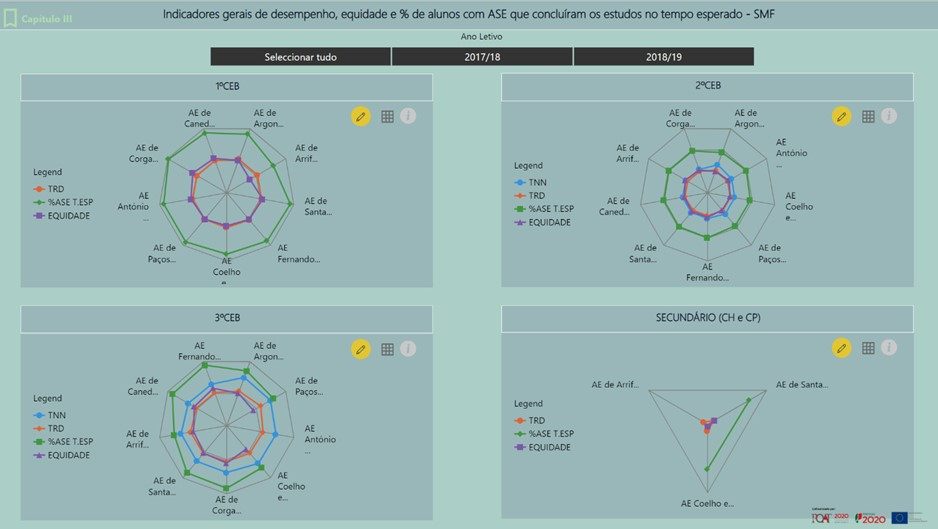
\includegraphics{C:/Users/julio/Documents/bookPoat/imagensRelatorio/figura55.jpg}
\caption{FIGURA 23: Capítulo III -- Leitura cruzada entre variáveis estritas e latas na aferição de níveis de sucesso em SMF por AE - FONTE: Infoescolas; Dados facultados pelo município de SMF}
\end{figure}

Complementarmente, o painel seguinte combina indicadores gerais de desempenho (TRD e TNN) com indicadores das 6 ações do PIICIE de SMF no que ao número de participantes diz respeito. A partir do desdobramento dos dados sobre os participantes, foi possível criar indicadores transversais ao nível das ações dos AE, assim como indicadores específicos por ação. A análise conjunta dos indicadores permite realizar um diagnóstico mais fiel dos AE e promover a reflexão sobre uma possível ligação com a participação nas ações.

\begin{figure}
\centering
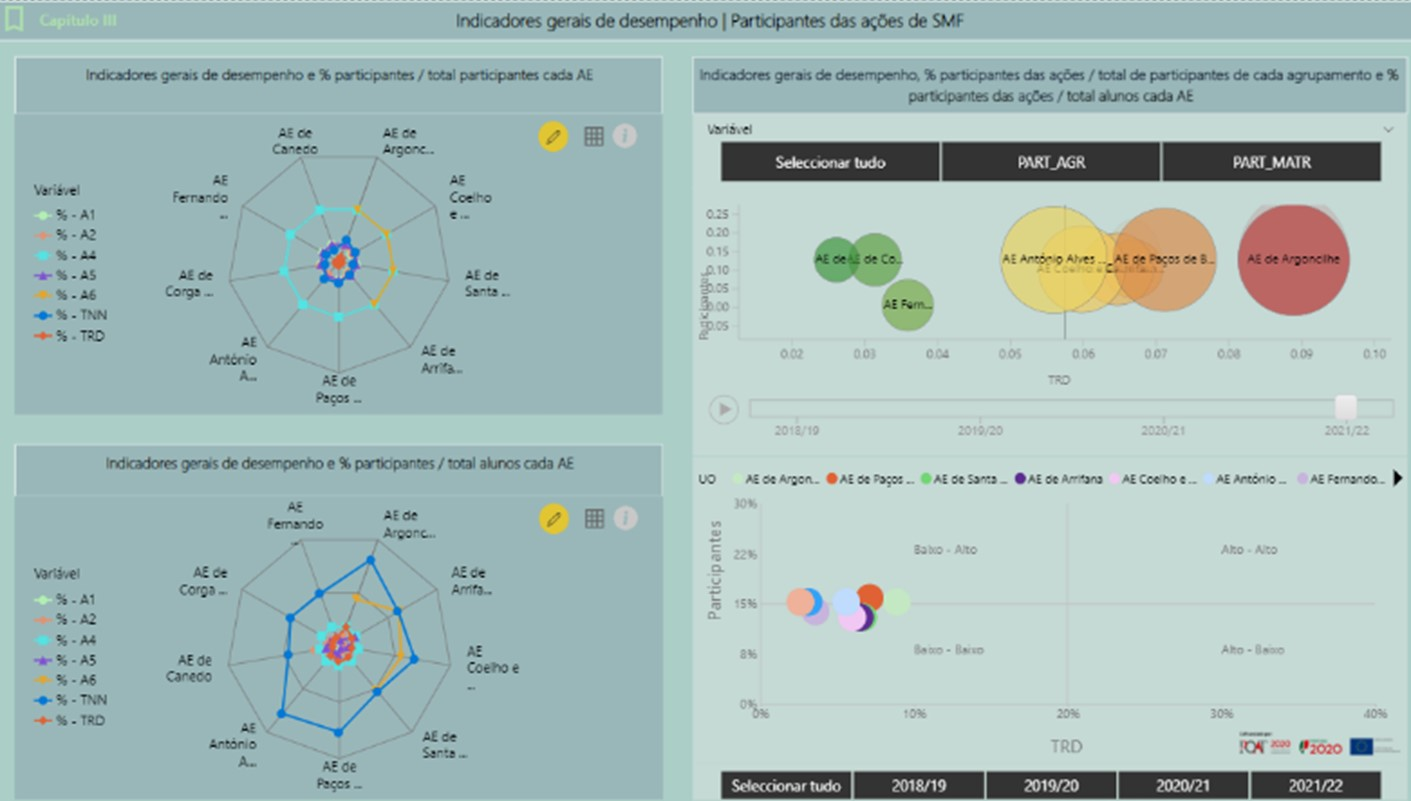
\includegraphics{C:/Users/julio/Documents/bookPoat/imagensRelatorio/figura56.jpg}
\caption{FIGURA 24: Capítulo III -- Leitura cruzada entre indicadores gerais de desempenho e indicadores transversais e específicos da participação nas ações do PIICIE de SMF por AE - FONTE: Infoescolas; Dados facultados pelo município de SMF}
\end{figure}

\hypertarget{indicadores-especuxedficos-de-caracterizauxe7uxe3o-das-auxe7uxf5es}{%
\section{\texorpdfstring{\textbf{Indicadores específicos de caracterização das ações}}{Indicadores específicos de caracterização das ações}}\label{indicadores-especuxedficos-de-caracterizauxe7uxe3o-das-auxe7uxf5es}}

Importa complexificar os indicadores de realização das ações, pelo que os indicadores específicos pretendem cumprir este papel. Alguns dos indicadores são comuns a todas as ações\footnote{Consultar Anexo VII.}, como é o caso dos parceiros envolvidos na formulação e/ou na elaboração e o número total de participantes já referido no ponto 4.2. Noutras ações procura especificar-se elementos associados quer aos participantes, quer aos domínios temáticos ou mesmo face a externalidades positivas que podem ser compreendidas à luz do PIICIE.

Seguem-se exemplos destes indicadores específicos, tal como apresentados nos painéis de informação construídos e disponibilizados no âmbito deste projeto, integrantes do capítulo IV.

\textbf{Ação 1 -- Equipa Multidisciplinar}

N.º de participantes\footnote{Consultar Anexo VIII.}

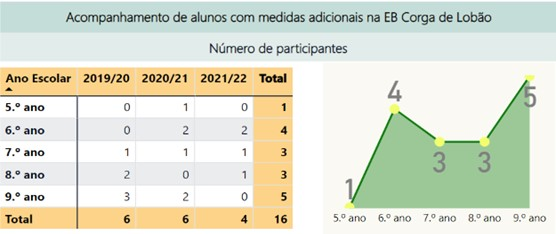
\includegraphics{C:/Users/julio/Documents/bookPoat/imagensRelatorio/figura57.jpg}

\begin{figure}
\centering
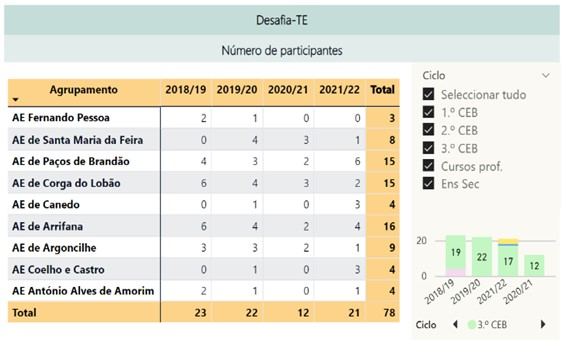
\includegraphics{C:/Users/julio/Documents/bookPoat/imagensRelatorio/figura58.jpg}
\caption{FIGURA 25: Capítulo IV -- Ação 1 do PIICIE, Participantes - FONTE: Dados facultados pelo município de SMF}
\end{figure}

Caracterização das atividades

No projeto de Acompanhamento de alunos com medidas adicionais na EB Corga de Lobão, nos três anos letivos analisados, num total de 16 participantes, a maioria dos alunos envolvidos pertencem ao 6º ano (4 participantes) e ao 9.º ano (5 participantes). O Desafia-TE obteve maior adesão no ano de 2018/19, sendo que em todos os anos o 3.º CEB destaca-se com um número maior de participantes.

\begin{figure}
\centering
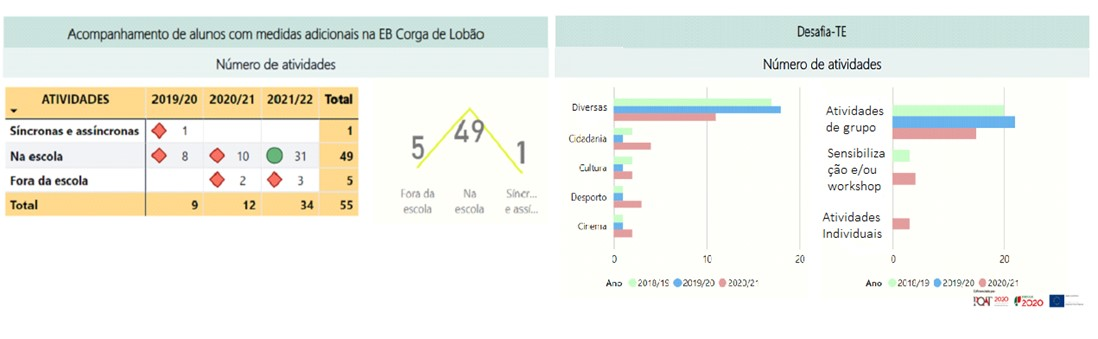
\includegraphics{C:/Users/julio/Documents/bookPoat/imagensRelatorio/figura59.jpg}
\caption{FIGURA 26: Capítulo IV -- Ação 1 do PIICIE, Caracterização das Atividades - FONTE: Dados facultados pelo município de SMF}
\end{figure}

Avaliação dos alunos abrangidos\footnote{Consultar Anexo VIII.}

No âmbito do Acompanhamento de alunos com medidas adicionais na EB Corga de Lobão, nos três anos letivos analisados, realizaram-se 55 atividades, das quais 49 foram desenvolvidas na escola. As atividades do Desafia-te compreenderam várias temáticas entre estas a cidadania, a cultura, o desporto e cinema. Foram realizadas 67 atividades no total, sendo que 57 são atividades de grupo, promovendo o trabalho em equipa e a partilha de experiências.

A equipa avaliou os alunos com medidas adicionais da EB Corga do Lobão em sete dimensões, destacando-se cinco pela sua importância: participação nas tarefas, empenho e realização das tarefas, aquisição e aplicação de conhecimentos, comportamento e relação com os pares e trabalho de equipa. Com base nestas avaliações, é possível ver o impacto das sessões ao longo dos três períodos, como se exemplifica na figura. A média do último período reflete o trabalho e a evolução dos alunos envolvidos.

\begin{figure}
\centering
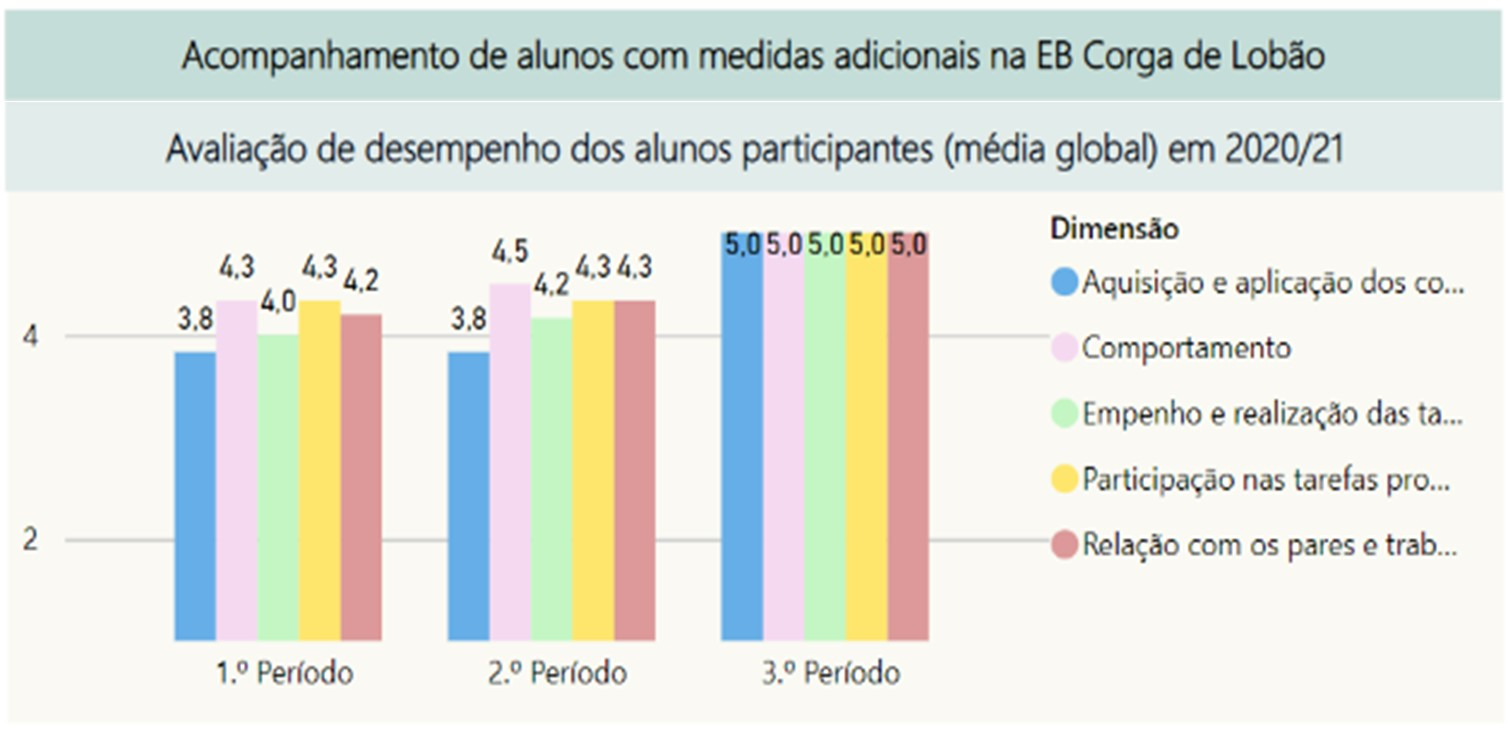
\includegraphics{C:/Users/julio/Documents/bookPoat/imagensRelatorio/figura60.jpg}
\caption{FIGURA 27: Capítulo IV -- Ação 1 do PIICIE, Avaliação dos alunos abrangidos - FONTE: Dados facultados pelo município de SMF}
\end{figure}

\textbf{Ação 2 -- Vive as Férias}

N.º de participantes

Esta ação abrange um grande público. O período que se destaca com o maior número de participantes, no total 1151 alunos, foi no verão de 2019. Verificou-se uma drástica redução nos anos seguintes devido à pandemia Covid-19, no entanto nota-se um aumento no verão de 2021 (602 participantes) uma vez que houve alívio de restrições relativamente à situação pandémica.

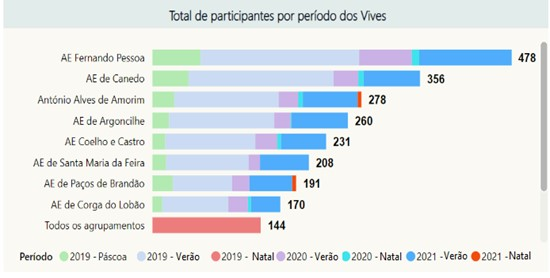
\includegraphics{C:/Users/julio/Documents/bookPoat/imagensRelatorio/figura61.jpg}

\begin{figure}
\centering
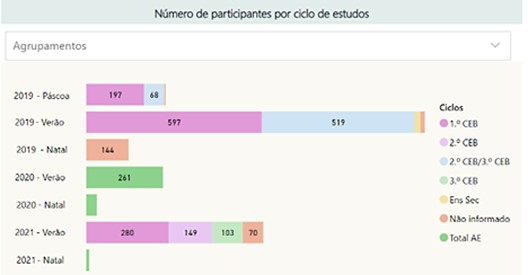
\includegraphics{C:/Users/julio/Documents/bookPoat/imagensRelatorio/figura62.jpg}
\caption{FFIGURA 28: Capítulo IV -- Ação 2 do PIICIE, Participantes - FONTE: Dados facultados pelo município de SMF}
\end{figure}

Caracterização das atividades

Nas atividades realizadas nos programas Vives, a área com maior destaque é o desporto. Procura-se, através deste tipo de atividades, fomentar uma prática regular de atividade física e a aquisição de diversas competências.

\begin{figure}
\centering
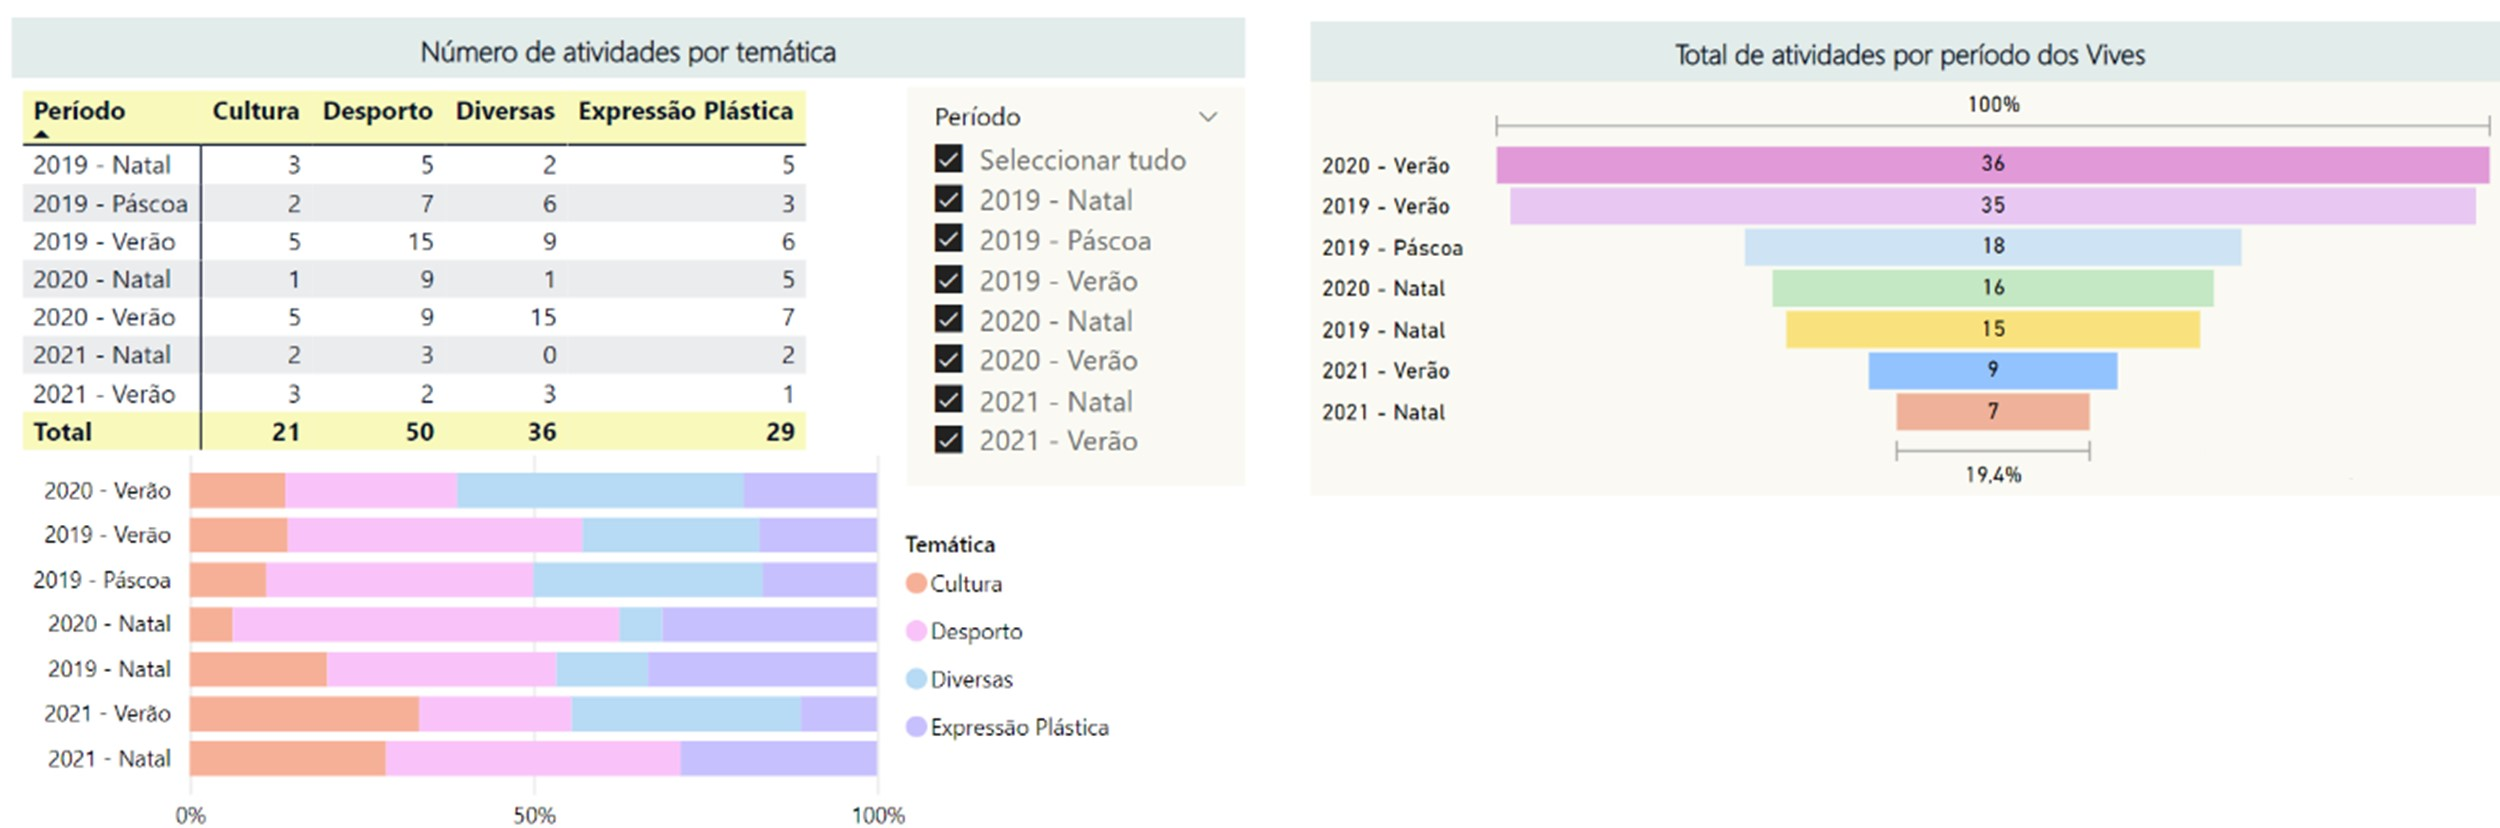
\includegraphics{C:/Users/julio/Documents/bookPoat/imagensRelatorio/figura63.jpg}
\caption{FIGURA 29: Capítulo IV -- Ação 2 do PIICIE, Caracterização das Atividades - FONTE: Dados facultados pelo município de SMF}
\end{figure}

\textbf{Ação 4 -- Educação 5.0}

N.º de alunos participantes nas Olimpíadas da Cidadania e do Património

A plataforma EDUFEIR@, criada no âmbito da ação Educação 5.0, ganhou mais relevância a partir de março de 2020, início da pandemia Covid-19. Esta ferramenta demonstrou-se útil para partilha de informação importante acerca do sistema educativo do município e para prestar apoio com conteúdos no âmbito da cidadania, património, apoio ao estudo e desafios. Na plataforma foi realizado o concurso Olimpíadas da Cidadania e do Património que alcançou, em 2019/20 e 2020/21, 657 participantes.

\begin{figure}
\centering
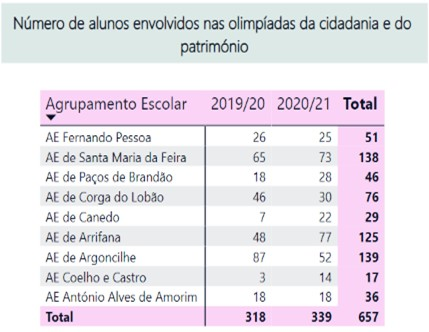
\includegraphics{C:/Users/julio/Documents/bookPoat/imagensRelatorio/figura64.jpg}
\caption{FIGURA 30: Capítulo IV -- Ação 4 do PIICIE, Participantes - FONTE: Dados facultados pelo município de SMF}
\end{figure}

N.º de acessos à plataforma EDUFEIR@

Os acessos à plataforma aumentaram exponencialmente em 2021 a partir de janeiro até meados do ano, coincidentes com a época em que decorrem as Olimpíadas da Cidadania e do Património.

\begin{figure}
\centering
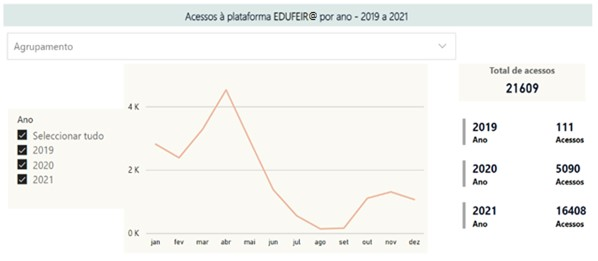
\includegraphics{C:/Users/julio/Documents/bookPoat/imagensRelatorio/figura65.jpg}
\caption{FIGURA 31: Capítulo IV -- Ação 4 do PIICIE, Acessos à Plataforma - FONTE: Dados facultados pelo município de SMF}
\end{figure}

Conteúdos temáticos na plataforma

A plataforma EDUFEIR@ tem conteúdos nas dimensões do património, cidadania e apoio ao estudo. Para além destas dimensões, disponibiliza diversos desafios e atividades em família dando a possibilidade dos alunos e famílias se divertirem e aprenderem juntos.

\begin{figure}
\centering
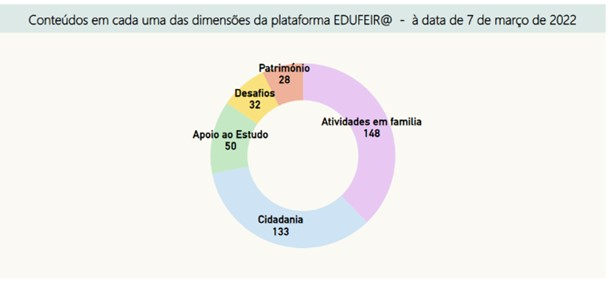
\includegraphics{C:/Users/julio/Documents/bookPoat/imagensRelatorio/figura66.jpg}
\caption{FIGURA 32: Capítulo IV -- Ação 4 do PIICIE, Conteúdos temáticos na Plataforma - FONTE: Dados facultados pelo município de SMF}
\end{figure}

N.º de tablets distribuídos

As escolas básicas foram equipadas com tablets (15 ou 26 tablets dependendo do nº de alunos da escola) de forma a potenciar a utilização das TIC e da plataforma EDUFEIR@ na aprendizagem em sala de aula.

\begin{figure}
\centering
\includegraphics{C:/Users/julio/Documents/bookPoat/imagensRelatorio/figura67.jpg}
\caption{FIGURA 33: Capítulo IV -- Ação 4 do PIICIE, Tablets distribuídos - FONTE: Dados facultados pelo município de SMF}
\end{figure}

\textbf{Ação 5 -- Hora de Programar}

N.º de alunos participantes

Com implementação em todos os Agrupamentos de Escolas, é nos AE de Arrifana, Paços de Brandão e Fernando Pessoa que a adesão aparenta ser mais massiva.

\begin{figure}
\centering
\includegraphics{C:/Users/julio/Documents/bookPoat/imagensRelatorio/figura68.jpg}
\caption{FIGURA 34: Capítulo IV -- Ação 5 do PIICIE, Participantes - FONTE: Dados facultados pelo município de SMF}
\end{figure}

Caracterização das atividades

Nesta ação realizaram-se atividades na área Computação e modularização, uso de software informático, bem como utilização de jogos para explicar conceitos teóricos. O domínio do uso de software informático destaca-se como a área com mais atividades realizadas (20 atividades).

\begin{figure}
\centering
\includegraphics{C:/Users/julio/Documents/bookPoat/imagensRelatorio/figura69.jpg}
\caption{FIGURA 35: Capítulo IV -- Ação 5 do PIICIE, Caracterização das Atividades - FONTE: Dados facultados pelo município de SMF}
\end{figure}

Participação em competições na área da Programação

No âmbito da ação Hora de programar os alunos do 1ºCEB e 2ºCEB estiveram envolvidos em duas atividades nacionais, o Roboeste e o Scratch. No total dos dois campeonatos participaram 292 alunos.

\begin{figure}
\centering
\includegraphics{C:/Users/julio/Documents/bookPoat/imagensRelatorio/figura70.jpg}
\caption{FIGURA 36: Capítulo IV -- Ação 5 do PIICIE, Participação em competições de programação - FONTE: Dados facultados pelo município de SMF}
\end{figure}

\textbf{Ação 6 -- Hora de Experimentar}

N.º de alunos participantes

Em 2018/19 estiveram envolvidos na Hora de Experimentar 433 alunos, sendo este o ano em que houve maior adesão. Em 2019/20 e 2020/21 participaram 404 e 411 alunos, respetivamente.

\begin{figure}
\centering
\includegraphics{C:/Users/julio/Documents/bookPoat/imagensRelatorio/figura71.jpg}
\caption{FIGURA 37: Capítulo IV -- Ação 6 do PIICIE, Participantes - FONTE: Dados facultados pelo município de SMF}
\end{figure}

Caracterização das atividades

Na Hora de Experimentar, as atividades desenvolvidas abrangem diversas áreas, como a alimentação e nutrição, zoologia, saúde e anatomia, química, entre outras. Tendo como objetivo, proporcionar experiências e explicar fenómenos do quotidiano aos alunos, a maioria das atividades da Hora de Experimentar são dedicadas à área da química.

\begin{figure}
\centering
\includegraphics{C:/Users/julio/Documents/bookPoat/imagensRelatorio/figura72.jpg}
\caption{FIGURA 38: Capítulo IV -- Ação 6 do PIICIE, Participantes - FONTE: Dados facultados pelo município de SMF}
\end{figure}

Níveis de aproveitamento dos alunos

O aproveitamento final dos alunos do 3º ano na disciplina de Estudo do Meio permitiu concluir que, nos anos letivos 2019/20 e 2020/21, cerca de 99,78\% e 99,56\% dos alunos, respetivamente, obteve bons resultados à disciplina, podendo existir uma relação com as sessões realizadas no âmbito desta ação.

\begin{figure}
\centering
\includegraphics{C:/Users/julio/Documents/bookPoat/imagensRelatorio/figura73.jpg}
\caption{FIGURA 39: Capítulo IV -- Ação 6 do PIICIE, Níveis de aproveitamento - FONTE: Dados facultados pelo município de SMF}
\end{figure}

\begin{figure}
\centering
\includegraphics{C:/Users/julio/Documents/bookPoat/imagensRelatorio/figura74.jpg}
\caption{FIGURA 40: Diagrama geral do quadro de ações do PIICIE de SMF -- Redes de agentes e Governação - FONTE: Dados facultados pelo município de SMF}
\end{figure}

\begin{figure}
\centering
\includegraphics{C:/Users/julio/Documents/bookPoat/imagensRelatorio/img11.jpeg}
\caption{FIGURA 41: Diagrama geral do quadro de ações do PIICIE de SMF -- Total de Participantes nas Ações - FONTE: Dados facultados pelo município de SMF}
\end{figure}

Para lá destes indicadores, a matriz de avaliação compreendia, no entanto, uma mais vasta bateria de indicadores específicos, quer de caracterização, quer de avaliação de cada uma das ações. Um dos principais desafios do presente estudo residiu, justamente, na recolha de informação que permitisse dar resposta a estes indicadores, formulados a \emph{posteriori}, não tendo sido contemplados no arranque do PIICIE. No \textbf{primeiro grupo de indicadores} há uma preocupação com a caracterização socioeducativa dos participantes, bem como com as especificidades de cada uma das atividades. No \textbf{segundo grupo de indicadores} pretender-se-ia medir, principalmente, os efeitos diretos (sobre os alunos envolvidos) e indiretos (sobre o universo alargado de alunos) de cada uma das ações.

Argumenta-se que estes indicadores facilitariam uma aferição mais exata do impacto do PIICIE, ainda que sem recorrer a metodologias como a avaliação de impacto ou a teoria da mudança. Ainda que a sua maioria não tenha sido operacionalizada, apresenta-se, de seguida, esta proposta.

\begin{figure}
\centering
\includegraphics{C:/Users/julio/Documents/bookPoat/imagensRelatorio/figura75.jpg}
\caption{QUADRO 1: Indicadores de caracterização e avaliação do impacto do PIICIE -- Proposta inicial - FONTE: GETIN-UA}
\end{figure}

\includegraphics{C:/Users/julio/Documents/bookPoat/imagensRelatorio/figura76.jpg}

Num esforço de formulação de indicadores transversais, que não secundarizem a especificidade, esboça-se uma proposta adicional. Ambiciona-se que esta possa ser operacionalizada numa miríade tão extensa quanto possível de programas de promoção do sucesso. Todos os indicadores propostos deverão ser considerados na avaliação \emph{ex ante}, avaliando-se a sua pertinência, acompanhados ao longo do processo (avaliação \emph{ongoing}) e apreciados no final do projeto (avaliação \emph{ex post}).

\begin{figure}
\centering
\includegraphics{C:/Users/julio/Documents/bookPoat/imagensRelatorio/figura77.jpg}
\caption{QUADRO 2: Indicadores de transversais de avaliação ex-ante, ongoing e ex-post do impacto do PIICIE -- Proposta adicional - FONTE: GETIN-UA}
\end{figure}

Deverão, ainda, ser considerados indicadores que, no futuro, com distância temporal, captem efeitos de longo prazo das medidas.

\hypertarget{impacto-da-pandemia-covid-19-na-execuuxe7uxe3o-das-atividades-e-projetos-programados}{%
\section{\texorpdfstring{\textbf{Impacto da pandemia Covid-19 na execução das atividades e projetos programados}}{Impacto da pandemia Covid-19 na execução das atividades e projetos programados}}\label{impacto-da-pandemia-covid-19-na-execuuxe7uxe3o-das-atividades-e-projetos-programados}}

Inevitavelmente, a pandemia obrigou a uma adaptação dos projetos e atividades compreendidos no PIICIE. O projeto Desafia-TE, integrado na ação Equipa Multidisciplinar foi ajustado e, a partir de março de 2020, transformou-se no programa ``Desafia-TE em casa'', que se concretizou através de seis sessões online no 3º período. Já os alunos abrangidos por medidas adicionais da EB Corga de Lobão continuaram a ter as sessões presencialmente, ainda que a escola estivesse encerrada devido ao confinamento imposto pela pandemia.

Em 2020 e 2021, não foi possível concretizar o programa Vives na interrupção letiva da Páscoa. Os programas Vives do Natal realizaram-se, porém houve uma limitação quanto ao número de participantes. No âmbito da ação Educação 5.0 ocorreram iniciativas orientadas para o próprio contexto pandémico como por exemplo, o \emph{workshop} ``A importância de atividade plásticas e lúdicas em tempos de quarentena'', realizado \emph{online}.

Nas ações da Hora de Programar e da Hora de Experimentar, criou-se um canal no \emph{Youtube} utilizado para disponibilizar a realização das atividades aos alunos, bem como a utilização da plataforma EDUFEIRA para o mesmo fim. Para além disso, foram fornecidas orientações das atividades para os alunos que não tinham acesso aos conteúdos.

\hypertarget{policy-recommendations}{%
\chapter{\texorpdfstring{\textbf{Policy recommendations}}{Policy recommendations}}\label{policy-recommendations}}

Avança-se com recomendações de políticas que não se circunscrevem ao território e ao PIICIE de Santa Maria da Feira, ainda que partam deste, das oportunidades e desafios identificados. Procura-se fazer o balanço do passado, retirando aprendizagens, em forma de sugestões e não de verdades absolutas, que possam melhorar as políticas cofinanciadas de promoção do sucesso.

No Programa Demografia, Qualificações e Inclusão, enquadrado pelo Portugal 2030, confirma-se a manutenção da aposta estruturante nas qualificações, uma vez que ``o baixo nível de qualificações de uma grande fatia da população continua a ser uma das maiores fragilidades estruturais'' (Portugal 2030, 2022). Assume-se que as recomendações que se seguem podem ser mobilizadas para o sistema de monitorização e avaliação das políticas de promoção do sucesso escolar, enquadradas pelo quadro 2021-2027.

\hypertarget{recomendauxe7uxf5es-sobre-o-combate-ao-insucesso-escolar}{%
\section{\texorpdfstring{\textbf{Recomendações sobre o combate ao insucesso escolar}}{Recomendações sobre o combate ao insucesso escolar}}\label{recomendauxe7uxf5es-sobre-o-combate-ao-insucesso-escolar}}

\leavevmode\vadjust pre{\hypertarget{hello}{}}%
PR1.1. Consolidação da visão territorial na promoção do sucesso escolar, quer através de uma análise estatística mais profunda e detalhada, quer de uma visão integrada de padrões e tendências supralocais

Num contexto de reforço de competências das CIM, importará consolidar uma visão que olhe para lá dos desafios municipais. Por outro lado, muitas vezes, a comparação exclusivamente dos indicadores de desempenho evidencia o cenário, mas não levanta hipóteses para as suas causas. Poderá ser útil adicionar outras variáveis ao diagnóstico territorial do (in)sucesso, como se procurou fazer no capítulo 3.

\leavevmode\vadjust pre{\hypertarget{hello}{}}%
PR1.2. Privilegiar domínios temáticos seletivos e os alunos do 1.º e do 2.º CEB como destinatários

No contexto de Santa Maria da Feira, aparenta estar em curso um esforço de definição de áreas estratégicas nos projetos educativos, começando pelo Plano Estratégico Educativo Municipal. O sucesso da ação Hora de Experimentar traduz-se numa apreciação positiva desta e no entendimento de que as futuras ações de promoção do sucesso escolar devem passar pelo domínio temático das Ciências Naturais e Experimentais.\footnote{Fonte: Inquérito preenchido pelos agentes na sessão final de projeto, 6 de outubro de 2022, Universidade de Aveiro.} Paralelamente, a Cidadania revela-se, atualmente, uma área de importância estratégica, assim com a Programação e Robótica.

O 1.º CEB tende a ser visto como o ciclo de estudos onde é mais prioritário desenvolver ações de promoção do sucesso, sendo partilhado pelos agentes a grande diferença entre o volume de medidas no 2.º CEB face ao 1.º CEB. A quebra significativa é, entre outros motivos, explicada pela maior carga horária. Não obstante, os agentes concordam na necessidade de direcionar mais ações para esse ciclo.\footnote{Fonte: Inquérito preenchido pelos agentes na sessão final de projeto, 6 de outubro de 2022, Universidade de Aveiro.}

\hypertarget{recomendauxe7uxf5es-para-os-programas-de-promouxe7uxe3o-do-sucesso-cofinanciados-no-quadro-2021-2027}{%
\section{\texorpdfstring{\textbf{Recomendações para os programas de promoção do sucesso cofinanciados no quadro 2021-2027}}{Recomendações para os programas de promoção do sucesso cofinanciados no quadro 2021-2027}}\label{recomendauxe7uxf5es-para-os-programas-de-promouxe7uxe3o-do-sucesso-cofinanciados-no-quadro-2021-2027}}

\leavevmode\vadjust pre{\hypertarget{hello}{}}%
Avaliação ex-ante

\leavevmode\vadjust pre{\hypertarget{hello}{}}%
PR2.1. Atualização do leque de indicadores de desempenho educativo, também designados por `Indicadores de resultado' nos Avisos do QFP 2014-20, de modo a incluir os indicadores de equidade

Aquando da formulação dos PIICIE e dos primeiros avisos (2016), os indicadores de equidade ainda não haviam sido formulados. Porém, estes ganharam força recentemente na aferição do sucesso escolar (DGEEC, 2022a; POCH, 2021). Devem, assim, ser integrados os seguintes indicadores, nos avisos e na implementação:

\begin{itemize}
\tightlist
\item
  Conclusão no tempo esperado;\\
\item
  Percursos diretos de sucesso;\\
\item
  Indicador de equidade.
\end{itemize}

O indicador de equidade (por comparação com as taxas de retenção e desistência e de níveis negativos) tende a ser encarado, pelos agentes, como o mais apropriado para a aferição do efeito dos programas de promoção do sucesso\footnote{Fonte: Inquérito preenchido pelos agentes na sessão final de projeto, 6 de outubro de 2022, Universidade de Aveiro.}.

\leavevmode\vadjust pre{\hypertarget{hello}{}}%
PR2.2. Consolidação do papel e posicionamento dos Municípios e das CIM como intermediários entre os órgãos de administração das escolas e as entidades de governo nacionais, designadamente no que diz respeito às estatísticas educativas

Os Municípios e CIM não serão bem-sucedidos, nem rigorosos, na formulação de estratégias educativas se não assumirem o conhecimento atualizado das suas realidades. Assim, fazendo uso da interoperabilidade de sistemas (e da crescente difusão de Observatórios Municipais de Educação), a candidatura aos programas de combate ao insucesso deve, desde logo, partir de um diagnóstico de desempenho educativo atualizado e pertinente, que permita identificar aspetos críticos da realidade educativa do território. Os Observatórios serão também essenciais na recolha e sistematização de informação para a monitorização dos programas.

Compreende-se que a DGEEC seja a \emph{gatekeeper} das estatísticas educativas, mas, perante um crescente contexto de descentralização de competências, não é irrazoável ambicionar um papel mais ativo das entidades subnacionais na organização e divulgação daquelas.

\leavevmode\vadjust pre{\hypertarget{hello}{}}%
PR2.3. Promoção de incentivos para a construção de metas e objetivos territorializados, que capturem e acompanhem a realidade socioeducativa abrangida pela ação.

A diversidade intrínseca dos territórios exige a formulação de indicadores em coerência com o diagnóstico. À elaboração do diagnóstico socioeducativo em resposta aos avisos de candidatura às ações cofinanciadas deve seguir-se uma consequente bateria de indicadores específicos, construída pela entidade beneficiária.

Para qualquer indicador devem ser contratualizados resultados esperados, assim como lançadas as bases para a recolha de dados longitudinais, sobre os participantes envolvidos, que facilitem a elaboração de avaliações de impacto, contemplando, por exemplo, níveis de aproveitamento e percurso dos alunos participantes.

\leavevmode\vadjust pre{\hypertarget{hello}{}}%
PR2.4. Robustecimento do diálogo entre a estratégia educativa do território e o PIICIE a implementar

Deve ser evitada a multiplicação de estratégias difusas, assegurando a convergência dos programas de combate ao insucesso com as estratégias escolares, municipais e intermunicipais implementadas que, por sua vez, deverão estar intimamente relacionadas com os desafios educativos territoriais. Esta perceção é partilhada pelos agentes educativos, entendendo-se que apenas deste modo será possível investir numa política educativa robusta, integrada e de continuidade.

\leavevmode\vadjust pre{\hypertarget{hello}{}}%
PR2.5. Garantia de condições de gestão e administração das entidades beneficiárias, de forma a aumentar a probabilidade de sucesso na implementação da operação

O sucesso do plano depende, em larga medida, dos Recursos Humanos mobilizados para a sua implementação e acompanhamento, entendimento partilhado pelos agentes. Sendo estes planos tão dependentes da interação interinstitucional entre atores, é crucial que estes apostem nos momentos de contacto e difusão. Esta necessidade torna-se mais premente em planos dinamizados por CIM, onde a rede é mais extensa.

Assim, será relevante definir e monitorizar, quantitativamente:

\begin{itemize}
\tightlist
\item
  Técnicos Superiores envolvidos no acompanhamento do plano;\\
\item
  Reuniões internas sobre o plano;\\
\item
  Reuniões da entidade beneficiária com entidades parceiras;\\
\item
  Instrumentos de avaliação;\\
\item
  Sessões abertas à comunidade educativa para divulgação do plano.
\end{itemize}

\leavevmode\vadjust pre{\hypertarget{hello}{}}%
Monitorização

\leavevmode\vadjust pre{\hypertarget{hello}{}}%
PR3.1. Acompanhamento e avaliação periódica da evolução do território nos indicadores de desempenho educativo e nos indicadores de realização das ações

Os relatórios anuais que as entidades beneficiárias remetem à autoridade de gestão, indicando as ações desenvolvidas durante esse período, deverão compreender a respetiva evolução nos indicadores de desempenho educativo. Sendo um dos desafios o desfasamento temporal na publicação de estatísticas educativas, torna-se ainda mais urgente a formalização de maiores competências das entidades subnacionais neste sentido \textbf{(PR 2.2)}.

Este esforço possibilita a identificação de desafios ao longo da implementação do PIICIE, conduzindo a pequenos ajustes do plano para fazer face àqueles. Não sendo desejáveis desvios significativos face ao estabelecido na memória descritiva do projeto, tais ajustes devem ser formulados com parcimónia.
Paralelamente, importa também encetar regularmente uma avaliação da execução face à previsão no que concerne os indicadores de realização de cada uma das ações, olhando para:

\begin{itemize}
\tightlist
\item
  Alunos participantes;\\
\item
  Encarregados de Educação participantes;\\
\item
  Docentes envolvidos;\\
\item
  Parcerias criadas;\\
\item
  Atividades realizadas.\footnote{Os indicadores propostos na PR2.5. devem também ser alvo desta monitorização anual.}
\end{itemize}

\leavevmode\vadjust pre{\hypertarget{hello}{}}%
PR3.2. Apreciação da eventual utilidade da mobilização de domínios e campos de análise da inspeção das escolas

Perante ações cujo sucesso depende de parcerias eficientes e lideranças capazes, poderá ser relevante mobilizar domínios da Liderança e Gestão para a monitorização dos planos de promoção do sucesso, quer nos seus resultados, quer nos indicadores propostos.

\leavevmode\vadjust pre{\hypertarget{hello}{}}%
PR3.3. Envolvimento dos agentes educativos na resposta periódica a inquéritos de aferição de preferências

Várias entidades beneficiárias procuraram perceber a satisfação dos envolvidos nos PIICIE através de inquéritos ou de questões mais abertas. Crê-se que estes inquéritos podem ganhar em detalhe e, consequentemente, em utilidade para a melhoria da política.

\leavevmode\vadjust pre{\hypertarget{hello}{}}%
Avaliação ex-post

\leavevmode\vadjust pre{\hypertarget{hello}{}}%
PR4.1. Avaliação final da evolução do território nos indicadores de desempenho educativo deve ser encarada como um ponto de partida para análises mais complexas

As entidades deverão prestar contas, no final da execução do projeto, sobre a evolução do território nas metas contratualizadas. Olhar para os indicadores de desempenho educativo não traduzirá de forma completa e fiel o efeito dos planos, uma vez que certamente não serão a única medida de promoção do sucesso. A própria terminologia ``indicadores de resultado'', adotada no quadro 2014-20, pode ser enganadora. Estes indicadores são, porém, essenciais para subsequentes ensaios de análises de correlação e causalidade mais sofisticadas.

\leavevmode\vadjust pre{\hypertarget{hello}{}}%
PR4.2. Disseminação dos resultados através de eventos públicos e da comunicação institucional

O inquérito difundido no evento final permitiu identificar a divulgação do PIICIE como um dos elementos menos bem conseguidos da sua implementação. Deve, por isso, ser encetado um esforço de divulgação das ações e dos respetivos resultados junto de toda a comunidade educativa do território em questão, assim promovendo a visibilidade do cofinanciamento europeu na área da Educação e evitando o encerramento dos projetos nas ``gavetas'' das entidades beneficiárias e parceiras.

\leavevmode\vadjust pre{\hypertarget{hello}{}}%
PR4.3. Retoma do processo de avaliação com distância temporal face ao fim do projeto, de modo a maximizar a captação de efeitos de longo prazo

Não é expectável que a política educativa introduza mudanças altamente disruptivas nem tampouco que os seus efeitos sejam imediatamente percetíveis. A aposta na implementação de um plano de promoção do sucesso junto de crianças do pré-escolar, por exemplo, terá efeitos de longo prazo que os processos de avaliação conduzidos logo após o término do projeto não conseguirão captar. A avaliação deve ser revisitada a médio prazo e, mais uma vez, assume relevância a recolha de dados longitudinais.

\hypertarget{recomendauxe7uxf5es-sobre-a-atuauxe7uxe3o-das-comunidades-intermunicipais}{%
\section{\texorpdfstring{\textbf{Recomendações sobre a atuação das Comunidades Intermunicipais}}{Recomendações sobre a atuação das Comunidades Intermunicipais}}\label{recomendauxe7uxf5es-sobre-a-atuauxe7uxe3o-das-comunidades-intermunicipais}}

Antecipa-se que as Comunidades Intermunicipais venham a reforçar a sua atuação no combate ao insucesso escolar. O POR Norte para o período de programação 2021-2027 já se encontra a preparar os Planos Intermunicipais de Promoção do Sucesso Escolar (PIPSE), sucessores dos PIICIE (CCDR-Norte, 2022), tal como acontece na região Centro (CCDR-Centro, 2022). Tal alteração tornaria as CIM e a AMP as únicas entidades beneficiárias destas políticas cofinanciadas (tal como já acontecia na região Centro), numa transferência que aparenta reforçar as suas responsabilidades. Este caminho deve, no entanto, ser trilhado com a consciência dos desafios subjacentes. Ademais, partilhas informais fazem crer na continuidade dos planos municipais.

\leavevmode\vadjust pre{\hypertarget{hello}{}}%
PR5.1. Reflexão sobre a exequibilidade de eleição de representantes municipais que trabalhem em conjunto com as CIM na implementação dos planos

As CIM são, amiúde, acusadas de défice democrático, o que pode beliscar a sua legitimidade (Gendźwiłł \& Lackowska, 2018). Nos últimos anos, a atribuição de renovadas competências às CIM, na área educativa, exigiu o reforço das redes de governança, assim garantindo a atuação conjunta de diferentes entidades políticas e atenuando as fragilidades que poderiam decorrer do estatuto das CIM. Um qualquer processo eletivo dos elementos das CIM, associado ao plano de promoção do sucesso, poderá aprofundar esta proximidade entre a CIM e as entidades educativas locais.

\leavevmode\vadjust pre{\hypertarget{hello}{}}%
PR5.2. Avaliação dos meios (financeiros e Recursos Humanos) necessários para as várias fases dos planos intermunicipais

Alguns contactos formais e informais com entidades intermunicipais beneficiárias de PIICIE permitiram inferir a insuficiência de Recursos Humanos para gerir uma operação que requer um elevado grau de articulação e acompanhamento. Assim, considera-se essencial esta avaliação preliminar e a posterior mobilização de meios em conformidade (em articulação com a PR2.5).

\hypertarget{referuxeancias-bibliogruxe1ficas-e-eletruxf3nicas}{%
\chapter*{\texorpdfstring{\textbf{REFERÊNCIAS BIBLIOGRÁFICAS E ELETRÓNICAS}}{REFERÊNCIAS BIBLIOGRÁFICAS E ELETRÓNICAS}}\label{referuxeancias-bibliogruxe1ficas-e-eletruxf3nicas}}
\addcontentsline{toc}{chapter}{\textbf{REFERÊNCIAS BIBLIOGRÁFICAS E ELETRÓNICAS}}

Agência para o Desenvolvimento e Coesão. (n.d.). Monitorização - Enquadramento. Obtido em 23 de agosto de 2022, de \url{https://www.adcoesao.pt/fundos/portugal-2020/monitorizacao/enquadramento/}

Allers, M. A., \& de Greef, J. A. (2017). Intermunicipal cooperation, public spending and service levels. Local Government Studies, 44(1), 127--150. \url{https://doi.org/10.1080/03003930.2017.1380630}

Câmara Municipal de Santa Maria da Feira (2022). Relatório Final de Candidatura PIICIE do Município de Santa Maria da Feira.

Carvalho, M., \& Joana, L. (2020). Uma análise comparada: sistemas inspetivos de alguns países. Revista Lusófona de Educação, 50(50), 27--41. \url{https://doi.org/10.24140/issn.1645-7250.rle50.02}

CCDR-Centro (2022). Programa Regional do Centro 2021-2027: Proposta. Obtido em 15 de setembro de 2022, de \url{https://www.consultalex.gov.pt/ConsultaPublica_Detail.aspx?Consulta_Id=253}

CCDR-Norte. (2022). Programa Regional do Norte 2021-2027: Proposta. Obtido em 15 de setembro de 2022, de \url{https://www.ccdr-n.pt/storage/app/media/uploaded-files/po20norte202030versc3a3oconsultapublica.pdf}

Decreto-Lei n.o 21/2019, de 30 de janeiro, do Ministério da Administração Interna. Diário da República n.o 21/2019, Série I (2019).

Decreto-Lei n.º 54/2018, de 6 de julho, da Presidência do Conselho de Ministros. Diário da República n.º 129/2018, Série I (2018).

Decreto-Lei n.o 7/2003, de 15 de janeiro, do Ministério das Cidades, Ordenamento do Território e Ambiente. Diário da República n.o 12/2003, Série I-A (2003).

Decreto-Lei n.o 72/2015, de 11 de maio, da Presidência do Conselho de Ministros. Diário da República n.o 90/2015, Série I (2015).

DGEEC, DGEstE, \& IGeFE. (2021). Carta Educativa, Guião para Elaboração. Obtido em 30 de maio de 2022, de \url{https://www.igefe.mec.pt/Files/DownloadDocument/17?csrt=5775597188220950806}

DGEEC. (2022a). Educação Inclusiva 2020/2021. Apoio à Aprendizagem e à Inclusão, escolas da rede pública do Ministério da Educação. Obtido em 23 de agosto de 2022, de \url{https://www.dgeec.mec.pt/np4/\%7B$clientServletPath\%7D/?newsId=1363\&fileName=EI2021_BreveSinteseResultados.pdf}

DGEEC. (2022a). Resultados Escolares: Sucesso e Equidade. Obtido em 13 de julho de 2022, de \url{https://www.dgeec.mec.pt/np4/\%7B$clientServletPath\%7D/?newsId=1359\&fileName=DGEEC_Relat_rio_Sucesso_Equidade_2022.pdf}

DGEEC. (2022b). Plano 21\textbar23 Escola+. Segundo relatório de monitorização. Obtido em 23 de agosto de 2022, de \url{https://www.dgeec.mec.pt/np4/\%7B$clientServletPath\%7D/?newsId=1369\&fileName=DGEEC_SegundoRelatorio_de_Monitorizacao_.pdf}

DGEEC. (2022b). Taxa de retenção e desistência (\%), por sexo, nível de ensino, ciclo de estudos e ano de escolaridade - Continente, NUTS II, III e Municípios -- 2003/04 a 2020/21. Obtido em 3 de agosto de 2022, de \url{https://www.dgeec.mec.pt/np4/248/}

Education Scotland. (2015). How good is our school? (4th edition). Obtido em 2 de setembro de 2022, de \url{https://education.gov.scot/improvement/documents/frameworks_selfevaluation/frwk2_nihedithgios/frwk2_hgios4.pdf}

Ehren, M., \& Shackleton, N. (2016). Risk-based school inspections: impact of targeted inspection approaches on Dutch secondary schools. Educational Assessment, Evaluation and Accountability, 28, 299--321. \url{https://doi.org/10.1007/s11092-016-9242-0}

Garrone, P., Grilli, L., \& Rousseau, X. (2012). Local Government Studies Management Discretion and Political Interference in Municipal Enterprises. Evidence from Italian Utilities. Local Government Studies, 39(4), 514-540. \url{https://doi.org/10.1080/03003930.2012.726198}

Gartner Glossary (n.d.). Information delivery. Obtido em 30 de setembro de 2022, de \url{https://www.gartner.com/en/information-technology/glossary/information-delivery}

Gaspar de Matos, M., Branquinho, C., Noronha, C., Moraes, B., Santos, O., Carvalho, M., Simões, C., Marques, A., Tomé, G., Guedes, F. B., Cerqueira, A., Francisco, R., \& Gaspar, T. (2022). Observatório de Saúde Psicológica e Bem-Estar: Monitorização e Ação. Obtido em 23 de agosto de 2022, de \url{https://www.dgeec.mec.pt/np4/\%7B$clientServletPath\%7D/?newsId=1357\&fileName=SaudePsi_final.pdf}

Gendźwiłł, A., \& Lackowska, M. (2018). A Borrowed Mandate? Democratic Legitimacy of Inter-municipal Entities: A Comparative Analysis. In F. Teles \& P. Swianiewicz (Eds.), Inter-Municipal Cooperation in Europe (pp.~57--77). Palgrave Macmillan. \url{https://doi.org/10.1007/978-3-319-62819-6}

IESE, ISCTE, \& PPLL Consult. (2021). Avaliação do Contributo do PT2020 para a Promoção do Sucesso Educativo, Redução do Abandono Escolar Precoce e Empregabilidade dos Jovens.

INE. (2021). População residente (N.o) por Local de residência, Sexo e Níveis de ensino; Decenal - INE, Recenseamento da população e habitação - Censos 2021. Obtido em 23 de agosto de 2022, de \url{https://www.ine.pt/xportal/xmain?xpid=INE\&xpgid=ine_indicadores\&indOcorrCod=0011168\&xlang=pt}

Inspeção-Geral da Educação e Ciência (IGEC). (2016). Quadro de referência para a avaliação externa das escolas. Obtido em 23 de agosto de 2022, de \url{https://www.igec.mec.pt/upload/AEE_2016-2017/AEE_16_17_(1)_Quadro_de_Referencia.pdf}

Inspeção-Geral da Educação e Ciência (IGEC). (2018a). Terceiro Ciclo da Avaliação Externa das Escolas - Âmbito, princípios e objetivos. Obtido em 23 de agosto de 2022, de \url{https://www.igec.mec.pt/upload/AEE3_2018/AEE_3_Amb_princ_objetivos.pdf}

Inspeção-Geral da Educação e Ciência (IGEC). (2018b). Terceiro Ciclo da Avaliação Externa das Escolas - Quadro de referência. Obtido em 23 de agosto de 2022, de \url{https://www.igec.mec.pt/upload/AEE3_2018/AEE_3_Quadro_Ref.pdf}

Ioannidou, A. (2010). Educational monitoring and reporting as governance instruments for evidence-based education policy. International Perspectives on Education and Society, 12, 155--172. \url{https://doi.org/10.1108/S1479-3679(2010)0000012011/FULL/XML}

Mairate, A. (2007). The `added value' of European Union Cohesion policy. Regional Studies, 40(2), 167--177. \url{https://doi.org/10.1080/00343400600600496}

Marques, J. L., Neves, R., Grifo, A., Duarte, J., Malta, J., Sousa, M. P., \& Santos, S. (n.d.). Plano Estratégico Educativo Municipal de Santa Maria da Feira 2022-2030.

Marques, J. L., Wolf, J., Borges, M., \& Batista, P. (2020). Sistemas de apoio à decisão em planeamento: desafios metodológicos e conceptuais. TPU: Território, Planeamento e Urbanismo: Teoria e Prática, 2, 52--79. \url{https://doi.org/10.34624/TPU.V0I2.23720}

Microsoft Power, B. I. Versão: 2.109.844.0 64-bit (setembro de 2022)

Ministério da Educação, \& Inspeção-Geral da Educação (IGE). (2010). Quadro de referência para a avaliação de escolas e agrupamentos de escolas. Obtido em 23 de agosto de 2022, de \url{https://www.igec.mec.pt/upload/AEE_2011/AEE_10_11_Quadro_Referencia.pdf}

Ministério da Educação. (2011). Propostas para um novo ciclo de avaliação externa de escolas, Relatório Final, Grupo de Trabalho para a Avaliação Externa das Escolas 2011. Obtido em 23 de agosto de 2022, \url{https://www.igec.mec.pt/upload/AEE2_2011/AEE2_GT_2011_RELATORIO_FINAL.pdf}

Nóvoa, A. (2013). The Blindness of Europe: New Fabrications in the European Educational Space. SISYPHUS Journal of Education, 1(1), 104--123. \url{http://ec.europa.eu/europe2020/services/faqs/index_en.htm}

Oliveira, P., Clímaco, M., Carravilla, M., Sarrico, C., Azevedo, M., \& Oliveira, J. (2006). Relatório final da actividade do Grupo de Trabalho para Avaliação das Escolas Dezembro 2006. Obtido em 25 de agosto de 2022, de \url{https://www.igec.mec.pt/upload/Relatorios/AEE_06_RELATORIO_GT.pdf}

POCH. (2021). Novo indicador de equidade na educação. Obtido em 13 de julho de 2022, de \url{https://www.poch.portugal2020.pt/pt-pt/Noticias/Paginas/noticia.aspx?nid=750}

Portugal 2030. (2022). Programa Demografia, Qualificações e Inclusão - Proposta de programa. Obtido em 26 de agosto de 2022, de \url{https://portugal2030.pt/wp-content/uploads/2022/07/PDQI_Versa\%CC\%83o-Submetida_Consulta-Pu\%CC\%81blica.pdf}

Presidência do Conselho de Ministros. (2018). ``Decreto-Lei 54/2018''. Diário da República 1ª série, 129 (julho): 2918 -- 2928. \url{https://data.dre.pt/eli/dec-lei/54/2018/07/06/p/dre/pt/html}

R Core Team (2022). R: A language and environment for statistical computing. R Foundation for Statistical Computing. Obtido de \url{https://www.R-project.org/}

Santos, S., Duarte, J. \& Marques, J. L. (2019). Quadro de referência aplicado aos instrumentos de gestão da rede e da política educativa à escala local. Revista de Desarrollo Sustentable, Negocios, Emprendimiento y Educación, 1(1), 1--19.

The Educational Institute of Scotland (EIS). (2019). Education Scotland Inspections. Obtido de 23 de agosto de 2022, de \url{https://education.gov.scot/education-scotland/what-we-do/inspection-and-review/standards-and-evaluation-framework/08-what-do-we-focus-on-during-inspection-and-review/\#:~:text=We\%20take\%20into\%20account\%20the,the\%20capacity\%20for\%20continuous\%20improvement}

Verdasca, J. (2020). Contributos para o desenvolvimento de um sistema de auto e multirregulação educativa. Revista Portuguesa de Investigação Educacional, n.o Especial, 111--143. \url{https://doi.org/10.34632/investigacaoeducacional.2020.8503}

Wickham, H., \& Grolemund, G. (2016). R for data science: import, tidy, transform, visualize, and model data. O'Reilly Media, Inc.~

XXI Governo -- República Portuguesa (2019). Modelo de Avaliação Externa das Escolas -- novo ciclo / Avaliação externa alargada às escolas profissionais privadas e às escolas com contrato de associação/patrocínio. Nota à Comunicação Social. Obtido em 23 de agosto de 2022, de \url{https://www.portugal.gov.pt/download-ficheiros/ficheiro.aspx?v=\%3D\%3DBAAAAB\%2BLCAAAAAAABAAzN7Q0AQCs6SFGBAAAAA\%3D\%3D}

\hypertarget{anexos}{%
\chapter*{\texorpdfstring{\textbf{ANEXOS}}{ANEXOS}}\label{anexos}}
\addcontentsline{toc}{chapter}{\textbf{ANEXOS}}

I -- Especificidades para instrumentalização dos indicadores gerais de resultado dos PIICIE e dos indicadores de caracterização socioeducativa

\begin{figure}
\centering
\includegraphics{C:/Users/julio/Documents/bookPoat/imagensRelatorio/figura79.jpg}
\caption{FONTE: GETIN-UA}
\end{figure}

\begin{figure}
\centering
\includegraphics{C:/Users/julio/Documents/bookPoat/imagensRelatorio/figura80.jpg}
\caption{FONTE: GETIN-UA}
\end{figure}

II -- Momentos de contacto e disseminação do projeto

\includegraphics{C:/Users/julio/Documents/bookPoat/imagensRelatorio/figura81.jpg}

\includegraphics{C:/Users/julio/Documents/bookPoat/imagensRelatorio/figura82.jpg}

III -- Avaliação Externa das Escolas em Portugal -- Domínios e campos de análise

\begin{figure}
\centering
\includegraphics{C:/Users/julio/Documents/bookPoat/imagensRelatorio/figura83.jpg}
\caption{FONTE: Inspeção-Geral da Educação e Ciência (IGEC)}
\end{figure}

Notas: 1° Ciclo\footnote{Ministério da Educação \& Inspeção-Geral da Educação (IGE) (2010); Oliveira et al.~(2006), Secção A-5.}, 2° Ciclo\footnote{Inspeção-Geral da Educação e Ciência (IGEC) (2016); Ministério da Educação (2011).} e 3° Ciclo\footnote{Inspeção-Geral da Educação e Ciência (IGEC) (2018b).}.

IV -- Operações aprovadas no QFP 2014-2020, enquadradas no OT10, executadas por entidades de Santa Maria da Feira

\begin{figure}
\centering
\includegraphics{C:/Users/julio/Documents/bookPoat/imagensRelatorio/figura84.jpg}
\caption{FONTE: PROJETOS APROVADOS DO PO NORTE, DE ACORDO COM A BASE DE DADOS ATUALIZADA A 31/08/2021}
\end{figure}

\includegraphics{C:/Users/julio/Documents/bookPoat/imagensRelatorio/figura85.jpg}

\begin{figure}
\centering
\includegraphics{C:/Users/julio/Documents/bookPoat/imagensRelatorio/figura86.jpg}
\caption{FONTE: PROJETOS APROVADOS DO POCH, DE ACORDO COM A BASE DE DADOS ATUALIZADA A 31/12/2021}
\end{figure}

V -- Taxas de cofinanciamento no quadro financeiro plurianual 2014-2020

\includegraphics{C:/Users/julio/Documents/bookPoat/imagensRelatorio/figura87.jpg}

No que concerne não o número de operações, mas o volume de cofinanciamento aprovado para os PIICIE, em cada região, importa considerar as diferentes taxas de cofinanciamento regionais, por via dos níveis de desenvolvimento, traduzidos através do PIB per capita. Consideradas menos desenvolvidas, as regiões do Norte, Centro, Alentejo e Açores podem ter um cofinanciamento europeu até 85\%, enquanto o Algarve (região em transição) tem cofinanciamento até 80\% e Lisboa, por ser mais desenvolvida, tem cofinanciamentos até 50\%. Por fim, a região da Madeira, ainda que o seu PIB per capita a torne uma região mais desenvolvida, é simultaneamente uma região ultraperiférica, pelo que as suas taxas de cofinanciamento podem também alcançar 85\%.

VI -- Elementos principais das ações do PIICIE de Santa Maria da Feira

\includegraphics{C:/Users/julio/Documents/bookPoat/imagensRelatorio/figura88.jpg}

\includegraphics{C:/Users/julio/Documents/bookPoat/imagensRelatorio/figura89.jpg}

VII -- Indicadores comuns e específicos das ações

\begin{figure}
\centering
\includegraphics{C:/Users/julio/Documents/bookPoat/imagensRelatorio/figura90.jpg}
\caption{FONTE: GETIN\_UA (ORIGEM DOS DADOS: CMSMF, 2022}
\end{figure}

VIII -- Esquemas associados à caracterização específica da Ação 1

Ação 1 - Equipa Multidisciplinar

Avaliação de desempenho dos alunos com medidas adicionais da EB Corga do Lobão (Média Global)

\begin{figure}
\centering
\includegraphics{C:/Users/julio/Documents/bookPoat/imagensRelatorio/figura91.jpg}
\caption{FONTE: GETIN\_UA (ORIGEM DOS DADOS: CMSMF, 2022}
\end{figure}

Participantes Desafia-TE por ciclo (atividade integrada na Ação 1 do PIICIE)

\begin{figure}
\centering
\includegraphics{C:/Users/julio/Documents/bookPoat/imagensRelatorio/figura92.jpg}
\caption{FONTE: GETIN\_UA (ORIGEM DOS DADOS: CMSMF, 2022}
\end{figure}

IX -- Esquemas adicionais associados às policy recommendations

\leavevmode\vadjust pre{\hypertarget{hello}{}}%
PR2.4. Robustecimento do diálogo entre a estratégia educativa do território e o PIICIE a implementar

Recomenda-se a seguinte articulação de estratégias:

\begin{figure}
\centering
\includegraphics{C:/Users/julio/Documents/bookPoat/imagensRelatorio/img13.jpg}
\caption{FONTE: GETIN\_UA (ORIGEM DOS DADOS: CMSMF, 2022}
\end{figure}

Deve, ainda, ser preenchida, em sede de candidatura, uma grelha semelhante à seguinte:

\begin{figure}
\centering
\includegraphics{C:/Users/julio/Documents/bookPoat/imagensRelatorio/figura93.jpg}
\caption{FONTE: GETIN\_UA (ORIGEM DOS DADOS: CMSMF, 2022}
\end{figure}

X -- Outputs complementares produzidos ao longo do período de execução do projeto

\textbf{Apresentações em conferências e congressos científicos:}

\begin{itemize}
\item
  `Os fundos comunitários e a política educativa em Portugal no quadro 2014-2020: Mapeamento das operações PIICIE', no 28.º Congresso da Associação Portuguesa de Desenvolvimento Regional (APDR) -- Green and inclusive transitions in Southern European regions: What can we do better, realizado em Vila Real, entre 16 e 17 de setembro de 2021\footnote{A apresentação decorreu num período anterior ao início do projeto.}
\item
  `A monitorização de políticas educativas locais: o caso de um município da Área Metropolitana do Porto', no IV Colóquio Internacional de Ciências Sociais da Educação, realizado em Braga, entre 12 e 14 de maio de 2022
\item
  `Desafios do processo de avaliação ex-post de uma política educativa cofinanciada', no IV Colóquio Internacional de Ciências Sociais da Educação, realizado em Braga, entre 12 e 14 de maio de 2022
\item
  `Distribuição dos fundos estruturais associados à Educação no quadro 2014-2020 em Portugal: padrões e singularidades regionais das políticas educativas', no 29.º Congresso da APDR - Islands and peripheral territories: challenges in a moving geography and changing climate patterns, entre 29 e 30 de junho de 2022
\item
  `Oportunidades na redefinição de princípios para a programação de equipamentos educativos', no 29.º Congresso da APDR - Islands and peripheral territories: challenges in a moving geography and changing climate patterns, entre 29 e 30 de junho de 2022
\item
  `A influência da governação europeia da Educação nas políticas educativas portuguesas', na Porto International Conference on Research in Education 2022 (ICRE '22), entre 20 e 22 de julho de 2022
\end{itemize}

\textbf{Publicações de artigos científicos:}

\begin{itemize}
\item
  Artigo submetido, a aguardar revisão: `Os fundos comunitários e a política educativa em Portugal no quadro 2014-2020: Mapeamento das operações PIICIE'
\item
  Artigo submetido, a aguardar revisão: `Desafios do processo de avaliação ex-post de uma política educativa cofinanciada' nos proceedings do IV Colóquio Internacional de Ciências Sociais da Educação
\item
  Artigo aprovado, em fase de produção: `A influência da governação europeia da Educação nas políticas educativas portuguesas', nos proceedings da Porto International Conference on Research in Education 2022 (ICRE '22)
\end{itemize}

\textbf{Trabalhos académicos, no âmbito de unidades curriculares do Mestrado de Ciências de Dados para Ciências Sociais (Universidade de Aveiro):}

\begin{itemize}
\item
  `Painéis de informação sobre territórios educativos' (Unidade Curricular: Seminário)
\item
  `Taxas de retenção e desistência de 2018/19 da região Norte' (Unidade Curricular: Econometria Temporal e Espacial)
\end{itemize}

XI -- Convite para participação no evento de disseminação

\includegraphics{C:/Users/julio/Documents/bookPoat/imagensRelatorio/figura94.jpg}

XII -- Inquérito difundido pelos agentes educativos

\includegraphics{C:/Users/julio/Documents/bookPoat/imagensRelatorio/figura95.jpg}

\includegraphics{C:/Users/julio/Documents/bookPoat/imagensRelatorio/figura96.jpg}

  \bibliography{book.bib,packages.bib}

\end{document}
